\documentclass[11pt,a4paper]{article}

\usepackage[utf8]{inputenc}
\usepackage[T1]{fontenc}
\usepackage{lmodern}
\usepackage[margin=1in]{geometry}
\usepackage{microtype}
\usepackage{amsmath,amssymb}
\usepackage{booktabs}
\usepackage{graphicx}
\usepackage{xcolor}
\usepackage[numbers,sort&compress]{natbib}
\usepackage{hyperref}
\usepackage{enumitem}
\usepackage[font=small,labelfont=bf]{caption}
\usepackage{subcaption}
\usepackage{placeins}
\usepackage[normalem]{ulem}

\captionsetup{justification=justified,singlelinecheck=false}
\captionsetup[subfigure]{justification=centering,singlelinecheck=false}

\hypersetup{
  colorlinks=true,
  linkcolor=black,
  citecolor=blue,
  urlcolor=blue
}

\setlength{\textfloatsep}{10pt plus 2pt minus 2pt}
\setlength{\floatsep}{8pt plus 2pt minus 2pt}
\setlength{\abovecaptionskip}{4pt}
\setlength{\belowcaptionskip}{0pt}
\renewcommand{\topfraction}{0.95}
\renewcommand{\textfraction}{0.15}
\renewcommand{\floatpagefraction}{0.8}
\renewcommand{\bottomfraction}{0.5}

\newcommand{\E}{\mathbb{E}}
\newcommand{\Prob}{\mathbb{P}}
\newcommand{\dd}{\,\mathrm{d}}

% unmarked footnote (no superscript) for the first-page code-availability note
\newcommand\blfootnote[1]{%
  \begingroup
  \renewcommand\thefootnote{}\footnote{#1}%
  \addtocounter{footnote}{-1}%
  \endgroup
}

\title{Deep Learning of Robust Market Making \\ under Regime-Switching Order Flow}
\author{%
  Felipe Moret \quad Fabrizio Lillo \\[2pt]
  \small Scuola Normale Superiore di Pisa \\
  \small \texttt{felipebueno.moret@sns.it}, \;
  \texttt{fabrizio.lillo@sns.it}%
}
\date{}

\graphicspath{{figures/}{./}}

\begin{document}
\maketitle
\blfootnote{Code, trained models, and paper source are available at
\url{https://github.com/felipemoret77/robust-deep-market-making}.}

\begin{abstract}
Classical market-making strategies based on stochastic control, such as
the Avellaneda--Stoikov and the Gu\'{e}ant--Lehalle--Fernandez-Tapia (GLFT)
extension, provide closed-form quoting rules, but rest on assumptions that
break down at realistic microstructure timescales.  One of them is that
order flow is stationary, while empirical evidence points to the existence
of regimes, possibly associated with algorithmic execution of metaorders.
In this case, existing methods provide negative PnL.  In this paper, we
develop a deep reinforcement-learning market maker (RLMM)---a Rainbow-style
distributional DQN (C51) which is calibrated and tested in a
zero-intelligence limit order book.  We find that, in the stationary
setting, RLMM outperforms GLFT across the entire observed risk--return
frontier.  The RLMM is more robust to flow asymmetry than GLFT, but, like
any stationarily trained strategy, it still suffers large drawdowns from
inventory saturation under persistent directional imbalance.  Augmenting
the state of RLMM with two auxiliary signals---a Bayesian online
change-point filter over the directional flow bias and a queue-adjusted
quote-exposure imbalance---restores profitability.  A final scenario-bandit
step that reweights low-return regime scenarios further improves
performance under random-persistence and correlated-direction stress.
\end{abstract}

\section{Introduction}

Market makers are the intermediaries who keep modern electronic
markets liquid: they continuously post two-sided quotes, standing
ready to both buy and sell, and earn the bid--ask spread as
compensation for supplying immediacy to the rest of the market.  This
service is not riskless.  Every fill nudges the market maker's
inventory away from neutral, and an intermediary who accumulates a
large directional position is exposed to adverse price moves before
that position can be unwound.  The problem is harder still because
real order flow is neither stationary nor symmetric: liquidity demand
arrives in bursts, buy and sell pressure can persist for extended
stretches, and the prevailing regime can shift without warning.
Robust quoting must therefore contend not merely with average
conditions but with the non-stationary, regime-dependent flow that
dominates at microstructure timescales---a thread we develop across
the paper's staged training pipeline.

Market making is naturally framed as a sequential stochastic-control
problem: the market maker chooses bid and ask quotes, the market
responds with random order arrivals and cancellations, and the market
maker must trade off spread revenue against inventory risk.  The
canonical analytical benchmarks are Avellaneda--Stoikov
(AS)~\citep{avellaneda2008} and the
Gu\'{e}ant--Lehalle--Fernandez-Tapia (GLFT)
extension~\citep{gueant2013dealing,gueant2017optimal}, both of which
yield closed-form quoting rules under stylized assumptions: a
diffusive mid-price, exponentially decaying fill intensity in quote
distance, and stationary, approximately symmetric order flow; see
\citet{cartea2015algorithmic} and \citet{gueant2016financial} for
textbook treatments of optimal market making, and \citet{cartea2014buy}
for a formulation with adverse selection.  These models were
developed mainly for dealer markets, where a single intermediary
quotes to incoming clients.  Whether they remain useful in an
order-driven central limit order book (defined below) is not obvious
a priori, and assessing this is one objective of the paper.  These
assumptions are analytically convenient but typically go unverified at
microstructure timescales~\citep{lehalle2018market}, where flow is
episodic, persistent, and regime-dependent, and where execution
depends not only on the quote distance from the mid-price, but also on
tick discreteness, finite queue depth, and the priority rules by which
resting orders are matched~\citep{smith2003,farmer2005predictive}.
GLFT is therefore used in this paper as a strong analytical benchmark
rather than as a fully realistic structural model of market making in
such a book.

We study this problem in its most common modern venue, the limit
order book.  A limit order book (LOB) is a centralized record of all
outstanding buy and sell quotes for a given asset at an exchange,
organized by price and timestamp.  Orders sitting in the book are
called limit orders (LOs); orders that execute immediately against
existing quotes are market orders (MOs).  Most modern exchanges match
incoming flow according to price--time priority: at each price level,
the oldest resting order is executed first-in-first-out (FIFO).  A
market maker (MM) is an agent that continuously posts LOs on both
sides of the book, aiming to capture the bid--ask spread while keeping
the inventory---the net long or short position accumulated from
asymmetric fills---within tolerable bounds.  It is this LOB
market-making problem---and its robustness to the non-stationary order
flow that the stylized AS/GLFT assumptions omit---that the present
paper takes as its focus.

\paragraph{Related work.}
The use of deep reinforcement learning (RL) for market making has a
growing literature that complements the closed-form controllers above
by learning quoting policies directly from interaction.
\citet{spooner2018mm} train tabular and deep agents on historical
order-book data.  \citet{kolm2020modern} survey the broader role of RL
in finance and discuss market making as a canonical application, and
\citet{zhang2020deep} apply deep RL to systematic trading more
broadly.  \citet{gueant2019drl} apply deep RL to corporate-bond market
making, emphasizing scalability to high-dimensional inventory states.
More recently, \citet{gasperov2021signals,gasperov2021approaches}
study deep RL approaches for market making, and
\citet{sadighian2019deep} applies it to cryptocurrency market making,
while \citet{spooner2020robust} consider adversarial RL and worst-case
robustness, and \citet{ganesh2019rl} study RL market making in a
multi-agent dealer market.  The bulk of this literature evaluates
policies on historical LOB data and replaces genuine execution
dynamics with simplifying heuristics---for instance a fixed fill
probability at the touch, or a deterministic slippage function---that
abstract away queue position, price--time priority, and endogenous
price impact.  This approach has two limitations that are important for
our study.  First, the order-flow distribution is fixed by the data
and cannot be controlled, which makes it difficult to stress-test a
policy under counterfactual regimes such as persistent directional
imbalance.  Second, without a faithful execution mechanism, a fixed
history of order arrivals cannot be mapped to the fills that each
policy would actually have received under consistent queue and
priority dynamics.  Because simplified heuristics ignore FIFO
priority, they bias the comparison between policies.  We therefore
train and evaluate both the RL agent and the analytical benchmarks
inside the same queue-aware event-driven simulator, running each
policy on matched realizations of the order-flow process.

\paragraph{Contributions.}
\begin{itemize}[leftmargin=1.2em,itemsep=1pt,topsep=2pt]
\item We calibrate a GLFT policy to a queue-faithful event-driven
  LOB simulator via censored waiting-time estimation of the fill
  intensity and a volatility signature plot for the diffusion scale,
  and show that the resulting policy dominates the at-best baseline in
  risk--return terms across a broad range of risk-aversion levels.
\item We train a distributional Deep Q-Network (DQN) with a
  categorical representation of the return distribution (C51) on the same simulator, and
  show empirically that it outperforms GLFT on the entire observed
 risk--return frontier under paired-seed evaluation.
\item We identify inventory saturation under persistent directional
  order flow as the dominant failure of stationarily trained
  market-making agents and the GLFT benchmark.
\item We fine-tune the stationary-optimal controller on
 regime-switching market-order flow using two belief-style
  auxiliary signals: a Bayesian online change-point filter for the
  latent directional order flow bias and a queue-adjusted
  quote-exposure imbalance for the agent's own resting quotes.  This
  pipeline substantially restores profitability under
  regime-switching order flow.
\item We introduce a scenario-bandit robust fine-tuning step that
  upweights low-return regime scenarios and show that it improves the
  regime-trained controller under random-persistence and
  correlated-direction stress tests.
\end{itemize}

The remainder of the paper is organized as follows.
Section~\ref{sec:problem_setup} introduces our event-driven
zero-intelligence (Santa Fe) LOB simulator, calibrates the GLFT policy
through censored waiting-time estimation and a volatility signature
plot, benchmarks it against the at-best baseline, and presents first
evidence that the closed form breaks under static asymmetry and
persistent directional flow.  Section~\ref{sec:learning_formulation}
casts market making as a throttled semi-Markov decision process,
details the state, action, and reward, and describes the Rainbow
distributional DQN (C51) backbone, whose stationary-flow behavior
Section~\ref{sec:stationary_results} maps out along the DQN--GLFT
risk--return frontier to define the Algorithm~A controller.
Section~\ref{sec:robustness} then introduces the regime-switching flow
model and exposes the inventory-saturation failure of this
stationarily trained controller, which
Section~\ref{sec:nonstat_training} addresses through Algorithm~B
fine-tuning driven by a Bayesian change-point flow belief and a
queue-adjusted quote-exposure imbalance.
Section~\ref{sec:interpretability} interprets the resulting policy via
local value-function slices that reveal its learned inventory-skew and
regime-aware logic, and Section~\ref{sec:stress_tests} subjects it to
out-of-distribution persistence, random-persistence, and
correlated-direction stress tests.
Section~\ref{sec:scenario_bandit_finetuning} presents the Algorithm~C
scenario-bandit robust fine-tuning step that upweights low-return
regime scenarios, before a final section gathers the discussion and
conclusion; two appendices derive the Bayesian online flow filter
(Appendix~\ref{app:bayesian_flow_filter}) and the closed-form GLFT
misspecification curve (Appendix~\ref{app:glft_misspecification}).


\section{Problem Setup and Benchmarks}
\label{sec:problem_setup}

\paragraph{Market model.}
The core market simulator is a 
continuous-time, event-driven, zero-intelligence (ZI) LOB simulator, sometimes called Santa Fe model 
\citep{smith2003,farmer2005predictive}.  We briefly summarize the
model here; a comprehensive treatment, including the
empirical motivation for each parameter definition and its calibration, can be found in
\citet{bouchaud2018trades}.  Prices live on a discrete,
equally spaced grid whose spacing is the tick size, the minimum
price change of the LOB: each grid position corresponds to exactly
one admissible quote price, so all price-valued quantities (best
bid, best ask, MM quotes) vary in integer multiples of the tick
size, while queue depths are integer counts of resting unit lots at
each level.  The state of the LOB at any instant is the vector of
outstanding volumes at each price level on the bid and ask sides.
All orders---incoming LOs, MOs, and cancellations---are of unit size,
so order flow is fully described by event counts at each price level.
Three exogenous Poisson flows drive the book's evolution:
\begin{itemize}[leftmargin=1.2em,itemsep=1pt,topsep=2pt]
\item \textbf{Limit orders (LOs).} New LOs of a given side arrive as a
  Poisson process with a rate $\lambda$ per side per price level,
  restricted to a finite band of levels around the
  best quote from the opposite side.  An arriving LO joins 
  the queue at its submitted price under price--time priority.
\item \textbf{Market orders (MOs).} MOs arrive as a Poisson process of
  total intensity $2\mu$; each MO is a buy with probability
  $p_{\mathrm{buy}}$ and a sell with probability $1-p_{\mathrm{buy}}$.
  An MO consumes the oldest resting order at the opposite best.

\item \textbf{Cancellations.}  Each resting LO is canceled
 independently at a rate $\theta_{\mathrm{cxl}}$ per unit size, so that the total
   cancellation rate at a given price level scales linearly with its
  depth.
\end{itemize}
The parameter triple $(\lambda, \mu, \theta_{\mathrm{cxl}})$ together with
$p_{\mathrm{buy}}$ fully specifies the stochastic flow.

\paragraph{Implementation features.}
Beyond the above described events, the simulator is characterized by two
features needed for a faithful evaluation of market-making policies:
\begin{itemize}[leftmargin=1.2em,itemsep=1pt,topsep=2pt]
\item \textbf{Per-order queue tracking,} so that each fill is
  attributed to a specific resting order rather than to the aggregate
  depth at a level, and the MM's queue position is maintained
  consistently across events.
\item \textbf{Grid re-centering,} which shifts the numerical price
  support when the mid drifts, keeping the book representation stable
  over long episodes without altering the economic state.
\end{itemize}

\paragraph{Analytical benchmarks.}
The simplest benchmark strategy is the \emph{at-best baseline}, a
naive market-making strategy that posts at and
tracks the current best bid and ask and leaves orders resting until
they are filled.  The at-best baseline serves as a lower bound against
which both analytical and learned policies are measured, and we refer
to it by this name throughout, including in figure legends.

As the main benchmark, we implement the GLFT
policy~\citep{gueant2013dealing}, which 
 assumes that the fill intensity of a quote posted
at distance \(\delta\) in ticks from the mid decays exponentially,
\begin{equation}\label{eq:Lambda}
  \Lambda(\delta)=A e^{-\kappa \delta},
\end{equation}
where \(A>0\) is the baseline fill intensity and \(\kappa>0\) controls
how quickly the execution probability vanishes as the quote moves away
from the mid; here \(\delta\) is the quote offset relative to the
 mid-price reference, measured on the LOB price grid.  Under
the additional assumption of an exponential-utility (CARA) objective with
risk-aversion coefficient \(\gamma_{\mathrm{GLFT}} > 0\) and a diffusive mid-price with
volatility \(\sigma\), \citet{gueant2013dealing} show that the optimal 
quoted prices of the MM admit the closed form
\begin{align}
  p_t^{a}
  &= m_t
  + \frac{1}{\gamma_{\mathrm{GLFT}}}\log\!\left(1 + \frac{\gamma_{\mathrm{GLFT}}}{\kappa}\right)
  - \frac{2 q_t - 1}{2}
    \sqrt{\frac{\sigma^2\gamma_{\mathrm{GLFT}}}{2\kappa A}
      \left(1 + \frac{\gamma_{\mathrm{GLFT}}}{\kappa}\right)^{\!1+\frac{\kappa}{\gamma_{\mathrm{GLFT}}}}},
  \label{eq:glft_ask}\\[4pt]
  p_t^{b}
  &= m_t
  - \frac{1}{\gamma_{\mathrm{GLFT}}}\log\!\left(1 + \frac{\gamma_{\mathrm{GLFT}}}{\kappa}\right)
  - \frac{2 q_t + 1}{2}
    \sqrt{\frac{\sigma^2\gamma_{\mathrm{GLFT}}}{2\kappa A}
      \left(1 + \frac{\gamma_{\mathrm{GLFT}}}{\kappa}\right)^{\!1+\frac{\kappa}{\gamma_{\mathrm{GLFT}}}}},
  \label{eq:glft_bid}
\end{align}
where \(m_t\) is the reference LOB mid-price at time \(t\) and
\(q_t\in\mathbb{Z}\) is the agent's signed inventory.  The GLFT
derivation treats prices as continuous; in our implementation we
discretize $p_t^{b}$ and $p_t^{a}$ by rounding the bid down and the
ask up to admissible tick indices before submitting them to the LOB.

In this form, GLFT cleanly separates \emph{spread setting} from
\emph{inventory skew}: the term $\tfrac{1}{\gamma_{\mathrm{GLFT}}}\log(1+\gamma_{\mathrm{GLFT}}/\kappa)$
sets the baseline half-spread (common to both sides and independent
of inventory), while the square-root term, scaled by the
inventory-dependent factor $(2q_t \mp 1)/2$, generates the
asymmetric skew that pulls both quotes toward the side on which the
MM wants to reduce its position.  The execution parameters
\(A\) and \(\kappa\) are calibrated from simulated data (see the next paragraph), and \(\gamma_{\mathrm{GLFT}}\) is the only
free control parameter that generates an explicit risk--return sweep: the larger
$\gamma_{\mathrm{GLFT}}$, the more aggressive the inventory skew, and hence the tighter
the inventory control.
GLFT thus yields interpretable, inventory-aware quotes, which makes it
a strong benchmark.  Because it does not endogenize queue position,
price--time priority, or the discrete execution mechanics of a FIFO
LOB, it serves as a disciplined analytical baseline against which the
RL controller is evaluated inside a more realistic microstructure.

\paragraph{Data and calibration.}
GLFT calibration in a FIFO LOB is itself non-trivial.  We follow the
censored waiting-time approach proposed by
\citet{laruelle2013optimal,gueant2015general}, adapted to our
event-driven simulator.  The Santa Fe parameter triple
$(\lambda, \mu, \theta_{\mathrm{cxl}})$ is calibrated, following the methodology
of \citet{bouchaud2018trades}, from Level-3 data for the equity \textsc{amzn} (Amazon Inc.)
obtained from the LOBSTER dataset, covering 28 trading days from
1~August~2025 to 10~September~2025 (regular session 09:30--16:00 ET,
with the first and last 60 minutes excluded to remove open/close
effects), for a total of approximately $2.9\times 10^{7}$ Level-3
message events. The resulting values used throughout this paper are
\begin{equation}
  \lambda = 0.06, \qquad
  \mu = 0.10, \qquad
  \theta_{\mathrm{cxl}} = 0.02,
\end{equation}
expressed per unit of simulated time (seconds).  All data
used for the GLFT calibration
are then generated by the calibrated simulator itself, so that the
simulated book reproduces a realistic range of spreads and queue
depths.  The
calibration episodes are disjoint from the evaluation episodes, so
there is no leakage between calibration and benchmarking.

The main input of the GLFT strategy is the fill intensity of Eq.~\ref{eq:Lambda}. To estimate it, following the approach in \citet{laruelle2013optimal}, we proceed as follows: for each quote distance $\delta$, a probe limit order is observed
over a fixed window of length $\Delta T_{\mathrm{calib}}$, the same
for every probe.  For the $i$-th probe we denote by $\tau_i$ the
elapsed time from posting until the probe is filled, whenever that
happens within the observation window; if the window expires before
any fill, the observation is right-censored and $\tau_i$ is not
observed.  The probe is never canceled before $\Delta T_{\mathrm{calib}}$:
it rests passively in the book from posting until either it fills or
the window expires, at which point it is canceled and a fresh probe
is posted at the next window boundary.  We summarize each probe by the pair
\begin{equation}
  \tilde{\tau}_i = \min(\tau_i,\,\Delta T_{\mathrm{calib}}),
  \qquad
  I_i = \mathbf{1}\{\tau_i < \Delta T_{\mathrm{calib}}\},
\end{equation}
where $\tilde{\tau}_i$ is the effective exposure time contributed by
the probe (the full window if it was censored, the fill time
otherwise) and $I_i$ is the indicator of a non-censored fill.  Under
the exponential-rate assumption of GLFT, see Eq. \ref{eq:Lambda}, the maximum-likelihood
estimator of the intensity is then
\begin{equation}
  \hat{\Lambda}(\delta)=\frac{\sum_i I_i}{\sum_i \tilde{\tau}_i},
\end{equation}
the ratio of observed fills to total exposure time.  The inferred
curve depends on $\Delta T_{\mathrm{calib}}$: short windows give
steeper near-book estimates, while longer windows flatten the fit
as mid-price drift makes the fill intensity non-stationary
(time-varying), violating the constant-rate/exponential assumption
underlying the estimator
(Figure~\ref{fig:glft_calib}).  We choose $\Delta T_{\mathrm{calib}}$
small enough to keep the fill intensity approximately stationary but large enough to
accumulate statistics at the deepest probe distances, consistent
with \citet{laruelle2013optimal}.  Concretely, we set
$\Delta T_{\mathrm{calib}} = 0.5$ seconds of simulated time throughout:
the near coincidence of the fits for the $0.5\,\mathrm{s}$ and
$1\,\mathrm{s}$ windows in Figure~\ref{fig:glft_calib} indicates that
the estimated intensity is already stable at this scale, whereas the
fits flatten visibly for longer windows as mid-price drift
contaminates the estimate.

\begin{figure}[htbp]
  \centering
  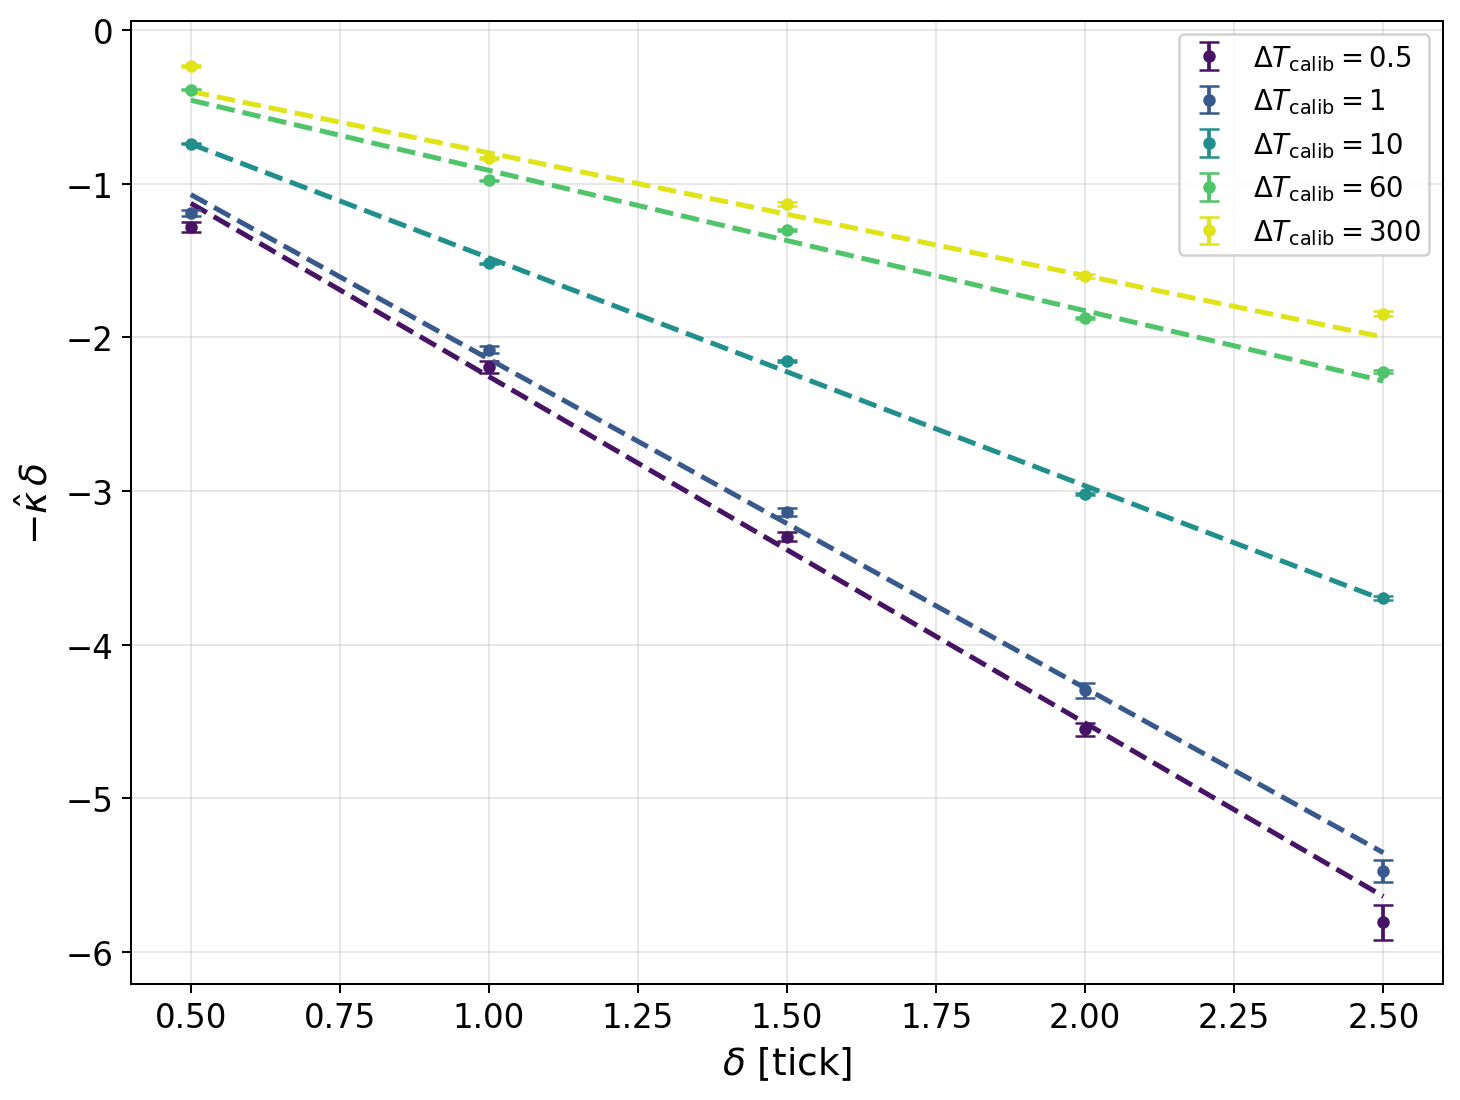
\includegraphics[width=0.7\linewidth]{censored_waiting_different_throttles.png}
  \caption{Censored waiting-time calibration of
  $\Lambda(\delta)=Ae^{-\kappa\delta}$ under five window durations
  $\Delta T_{\mathrm{calib}}$.  Points show the
  empirical linearized log-intensity per quote distance $\delta$,
  averaged over $N_{\mathrm{rep}}=20$ independent calibration runs;
  error bars are the standard error of the mean. Dashed lines are the
  log-linear regression fits.  Short windows yield steeper fits;
  long windows flatten due to mid-price drift within the observation
  window.}
  \label{fig:glft_calib}
\end{figure}

The probing scheme delivers an empirical intensity curve
$\{\hat{\Lambda}(\delta_k)\}_{k=1}^{K_\delta}$ over a finite grid of quote
distances $\delta_k$.  The GLFT parameters $(A, \kappa)$ are then
recovered by a least-squares fit of the exponential model
$\Lambda(\delta)=A\,e^{-\kappa\delta}$ in log-space.  For the
calibration window $\Delta T_{\mathrm{calib}} = 0.5\,\mathrm{s}$
adopted here, the fit yields
\begin{equation}
  \hat{A} = 0.1507\ \mathrm{s}^{-1},
  \qquad
  \hat{\kappa} = 2.335\ \mathrm{ticks}^{-1},
  \label{eq:glft_calib_values}
\end{equation}
and these are the values used for the GLFT benchmark throughout the
paper, as well as in the closed-form misspecification analysis of
Appendix~\ref{app:glft_misspecification}.

The volatility $\sigma$ entering the GLFT solution is not
a single-window variance estimator but is extracted from the
\emph{volatility signature plot}, a standard microstructure
diagnostic that reveals the timescale dependence of mid-price
diffusivity.  For a discrete mid-price series $\{m_t\}$ sampled on
the simulator clock and a lag $h$ in physical simulated-time units, the signature curve is
\begin{equation}
  \widehat\sigma(h)
  = \sqrt{\,\mathbb{E}\!\bigl[(m_{t+h}-m_t)^2\bigr]/h\,},
\end{equation}
estimated empirically by its sample analogue over all overlapping
increments of length $h$ in the calibration data.  For a pure
diffusion $dS_t = \sigma\,dW_t$ the curve is flat,
$\widehat\sigma(h) = \sigma$; in practice microstructure noise (bid--ask
bounce, tick discretization) inflates $\widehat\sigma(h)$ at small lags,
while at large lags the curve stabilizes at a plateau that reflects
the genuine long-horizon diffusion scale of the mid-price.  We take
$\sigma$ as the value of that plateau, thus avoiding
contamination from short-horizon microstructure effects that the
GLFT model does not capture. 
Applying this construction to the
simulator calibrated with the Santa Fe intensities
$(\lambda, \mu, \theta_{\mathrm{cxl}}) = (0.06, 0.10, 0.02)$ reported above
yields a plateau value
$\sigma_{\mathrm{plateau}} \approx 0.30 \;\mathrm{ticks}/\sqrt{\mathrm{s}}$,
which we adopt as the diffusion scale entering the GLFT
coefficients. 

\paragraph{Performance of analytical market making benchmarks.}
We run the two analytical market making benchmarks on numerical simulations of the LOB according to the Santa Fe model. Figure~\ref{fig:glft_vs_naive} reports a paired-seed
comparison over $N_{\mathrm{sim}} = 1000$ episodes of
$N_{\mathrm{steps}} = 5000$ LOB events each. We observe that GLFT clearly
dominates the at-best baseline in risk--return terms across a broad risk-aversion
range.   Two regularities
emerge: First, GLFT yields a small mean PnL advantage over the
at-best baseline only at the lowest risk aversion tested, and this
advantage reverses as risk aversion grows (paired Wilcoxon test on the
per-seed difference $\Delta = \mathrm{PnL}_{\mathrm{GLFT}} -
\mathrm{PnL}_{\text{at-best}}$ gives median $\Delta = +0.02$, $-0.015$,
$-0.10$ for $\gamma_{\mathrm{GLFT}} = 10^{-6}, 10^{-3}, 10^{-1}$, with
$p \approx 0.05$, $0.008$, $\ll 10^{-4}$).  At higher
$\gamma_{\mathrm{GLFT}}$ the inventory skew sacrifices spread capture
for a tighter inventory distribution, so the principal benefit of GLFT
over the at-best baseline is inventory control rather than mean PnL.  A
useful limiting case clarifies the role of the inventory-skew
term: as $\gamma_{\mathrm{GLFT}} \to 0$ the GLFT half-spread reduces to
$\approx 1/\kappa$ and the inventory-skew term
vanishes, so the GLFT quotes degenerate into essentially
unskewed touch-following quotes that closely resemble the at-best
baseline.  Empirically, the two policies then achieve a
comparable mean PnL in this risk-neutral limit, but the at-best
baseline exhibits a markedly wider PnL distribution, since its
inventory is left to drift unbounded in the absence of any active
inventory control.  Second, the variation of $\gamma_{\mathrm{GLFT}}$ traces the
expected risk--return trade-off: a larger $\gamma_{\mathrm{GLFT}}$ tightens
inventory control but sacrifices raw PnL, while a smaller $\gamma_{\mathrm{GLFT}}$
increases the expected return at the cost of greater inventory
risk.  Taken together, these results show that the classical
closed-form inventory-skew logic remains effective in an
event-driven stochastic simulator.

\begin{figure}[htbp]
  \centering
  \makebox[\linewidth][c]{%
  \begin{minipage}{1.18\linewidth}
  \centering
  \begin{subfigure}[t]{0.49\linewidth}
    \centering
    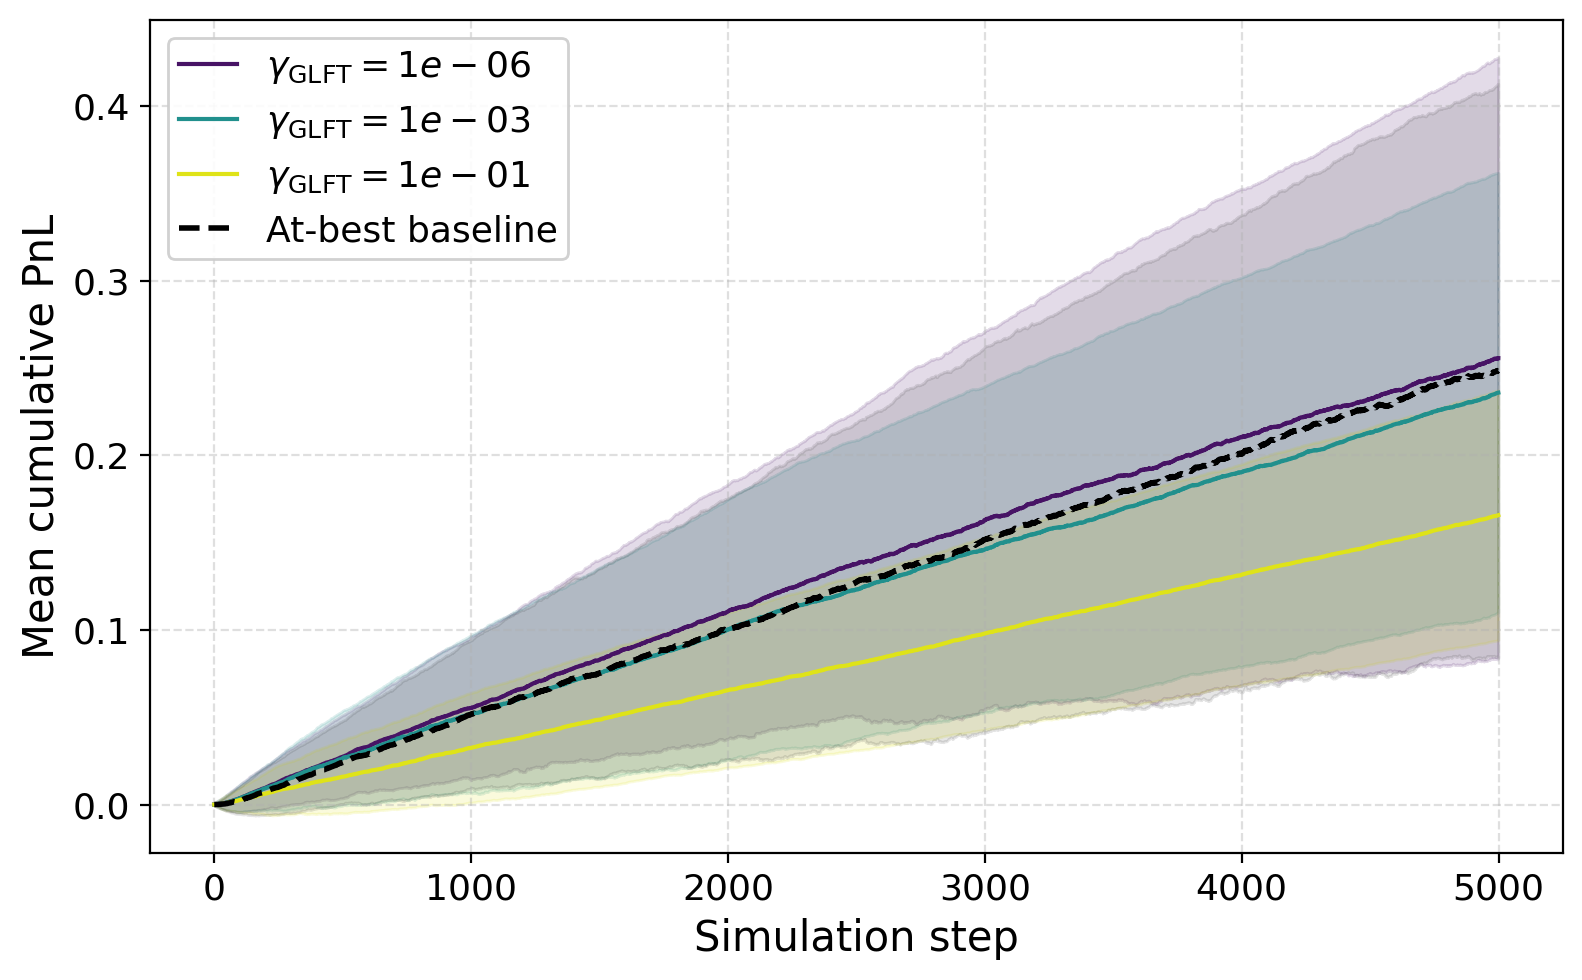
\includegraphics[width=\linewidth,height=6cm,keepaspectratio]{pnl_cumulated_pnl_glft_vs_naive.png}
    \caption{Mean cumulative PnL across simulations.}
    \label{fig:glft_pnl_cum}
  \end{subfigure}
  \hfill
  \begin{subfigure}[t]{0.49\linewidth}
    \centering
    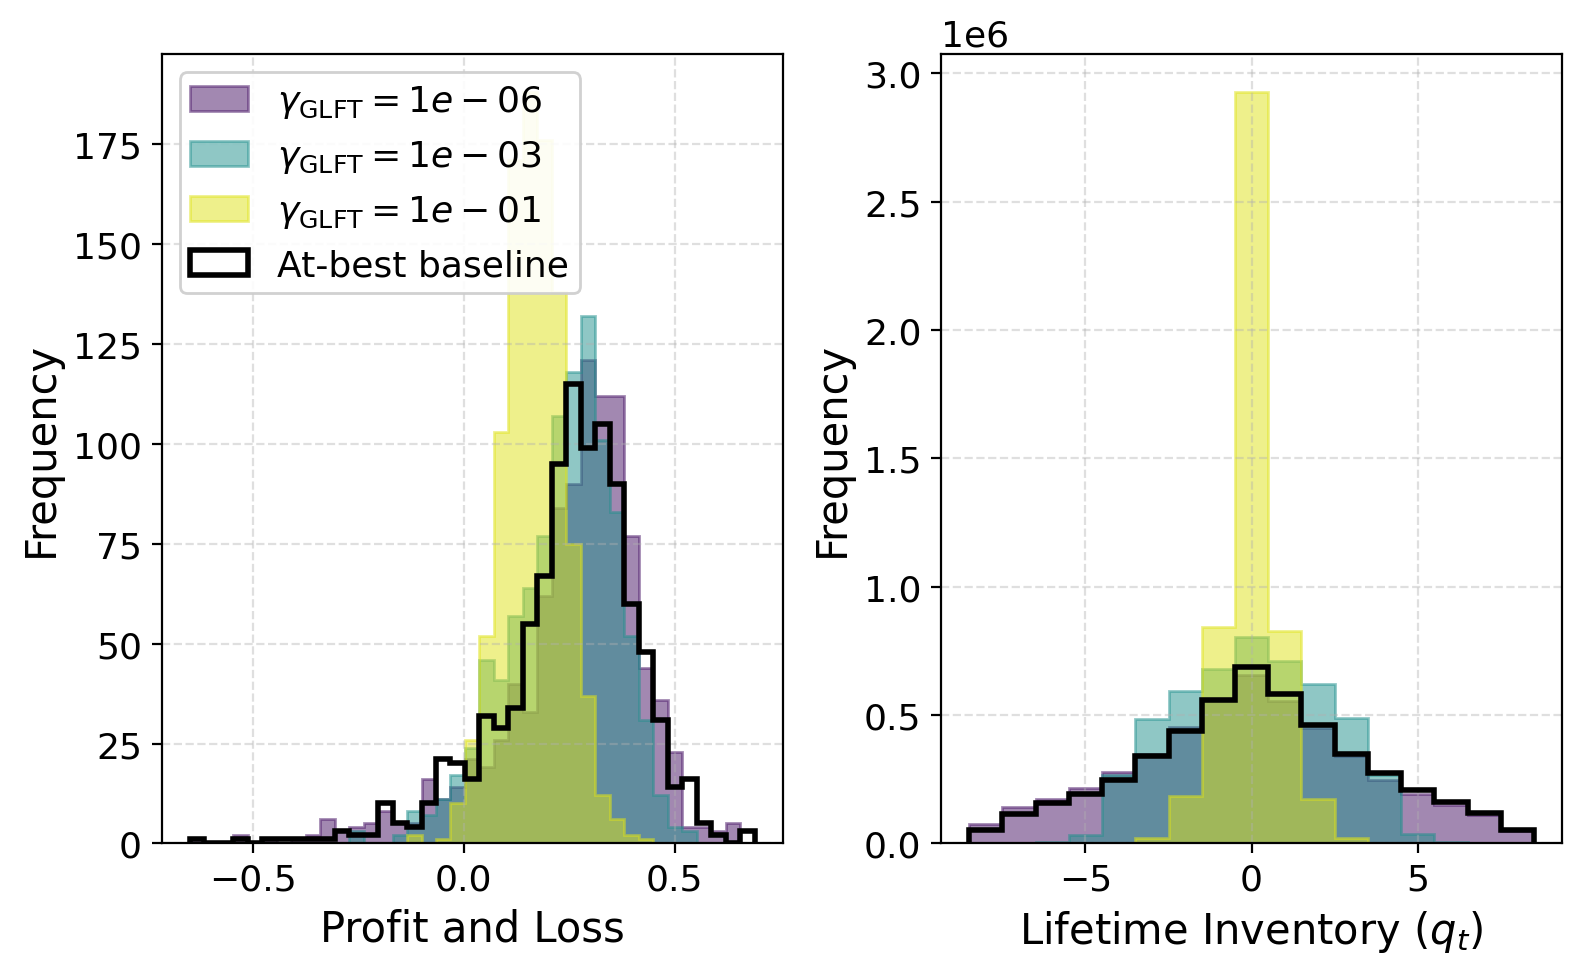
\includegraphics[width=\linewidth,height=6cm,keepaspectratio]{glft_naive_pnl_lifetime_hist.png}
    \caption{Terminal PnL and lifetime-inventory histograms.}
    \label{fig:glft_hist_joint}
  \end{subfigure}
  \end{minipage}}
  \caption{GLFT vs.\ the at-best baseline over $N_{\mathrm{sim}} = 1000$
  paired-seed episodes of $N_{\mathrm{steps}} = 5000$ LOB events, with
  $\gamma_{\mathrm{GLFT}}\in \{10^{-6}, 10^{-3}, 10^{-1}\}$.
  (\subref{fig:glft_pnl_cum}) Mean cumulative PnL.
  (\subref{fig:glft_hist_joint}) Terminal PnL (left) and
  lifetime inventory (right) histograms.
  }
  \label{fig:glft_vs_naive}
\end{figure}

\paragraph{Where the closed form breaks: persistent directional flow.}
The benchmark above inherits the stationarity of its market model:
the market-order flow is symmetric ($p_{\mathrm{buy}} = 0.50$) and its
directional mix is constant in time.  Empirically, neither property
is a faithful description of real order books: the directional bias
of the MO flow is highly non-stationary, with slowly varying regimes
of persistent buy or sell pressure---a regime-switching structure
with a long tradition in econometric modeling of non-stationary
series \citep{hamilton1989regime}.  These regimes are typically
driven by large institutional metaorders sliced into many child
trades and by crowding among correlated
participants~\citep{toth2015persistent,bouchaud2009digest,lillo2004longmemory};
recent microstructure studies of intraday MO flow identify discrete
regimes of directional imbalance separated by abrupt
transitions~\citep{tsaknaki2025online}, a structure that is
incompatible with the stationary Poisson model underlying GLFT and
AS models.

We first quantify the deterioration in PnL due to the assumption of a balanced market order flow when it is instead stationary but asymmetric ($p_{\mathrm{buy}} \neq 0.50$).
Figure~\ref{fig:misspec_comparison} quantifies this
misspecification cost as a function of the actual $p_{\mathrm{buy}}$. We observe that the expected PnL of a GLFT strategy peaks, as expected, at $p_{\mathrm{buy}} = 0.50$ but crosses into loss-making territory once the asymmetry
exceeds $|p_{\mathrm{buy}} - 0.50| \approx 0.08$. Interestingly, it is possible to obtain a closed-form approximation (see Appendix~\ref{app:glft_misspecification}) for the expected PnL, which is also reported in the figure.


The figure also shows the same quantity for the reinforcement-learning market maker (RLMM) presented in
Sections~\ref{sec:learning_formulation}--\ref{sec:stationary_results}, which instead remains profitable on a substantially wider band
($p_{\mathrm{buy}} \in [0.40, 0.60]$) but inherits the same
structural fragility.

\begin{figure}[htbp]
  \centering
  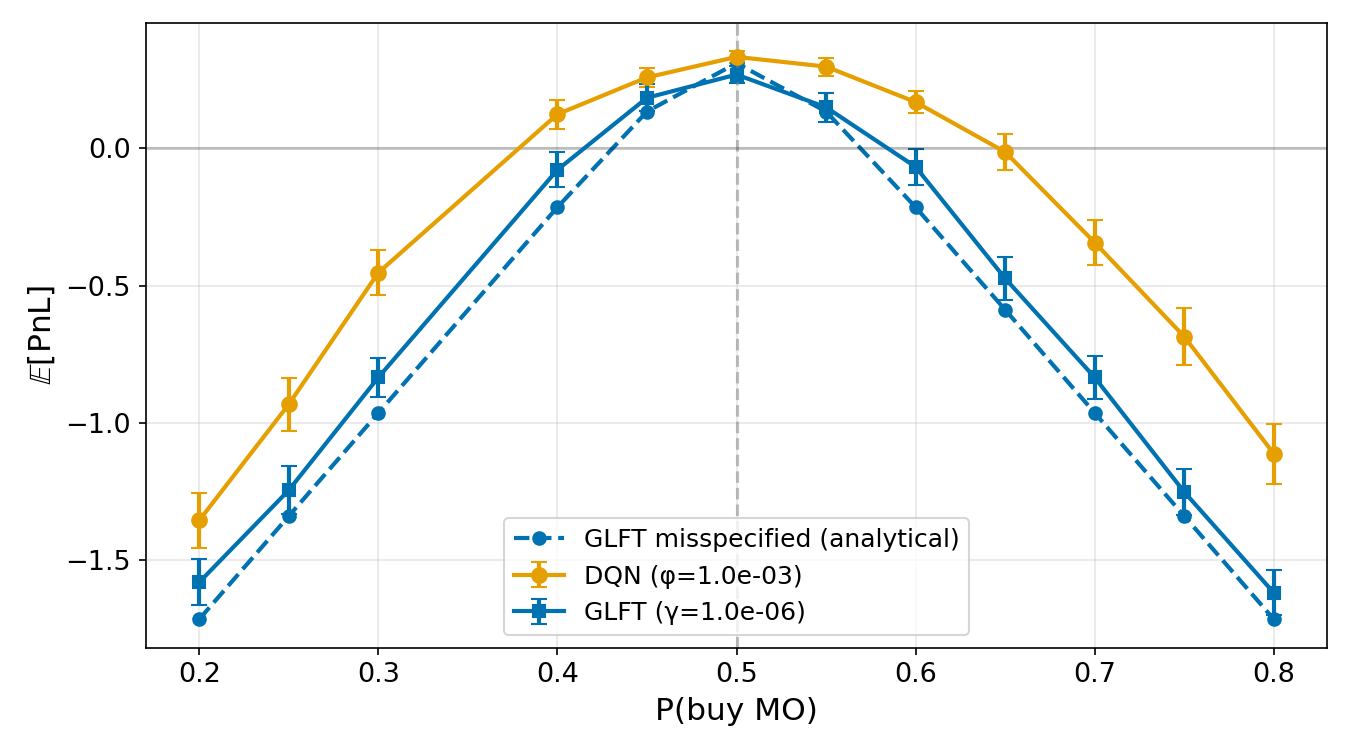
\includegraphics[width=0.7\linewidth]{dqn_vs_as_vs_glft.png}
  \caption{Expected  PnL as a function of $p_{\mathrm{buy}}$
  for the empirical GLFT benchmark (blue), and the
  closed-form GLFT-under-misspecification approximation of Appendix~\ref{app:glft_misspecification} (dashed blue).  The orange line is obtained implementing the RLMM strategy
  presented in
  Sections~\ref{sec:learning_formulation}--\ref{sec:stationary_results}.
  }
  \label{fig:misspec_comparison}
\end{figure}

The picture worsens when the imbalance \emph{persists}.
Figure~\ref{fig:glft_degradation_tau} evaluates the calibrated GLFT
policy under persistent directional regimes: the buy-MO probability
is piecewise-constant, held fixed within each regime, with regime
durations drawn exponentially with mean $\tau_r$ MO events (the
generative model is fully specified in
Section~\ref{sec:robustness}).  Terminal PnL decreases
monotonically as the persistence $\tau_r$ grows, turning a
profitable stationary strategy into a systematically loss-making
one---and no parameter of the closed form can absorb this, because
the quotes are flow-blind by construction.  This failure mode, not
the stationary comparison, is the central problem addressed in the
remainder of the paper: Sections~\ref{sec:learning_formulation}
and~\ref{sec:stationary_results} construct the controller and
establish that it dominates GLFT under stationary flow;
Sections~\ref{sec:robustness}--\ref{sec:scenario_bandit_finetuning}
then diagnose the controller's own regime fragility and repair it
with an online flow belief and robust fine-tuning.

\begin{figure}[htbp]
  \centering
  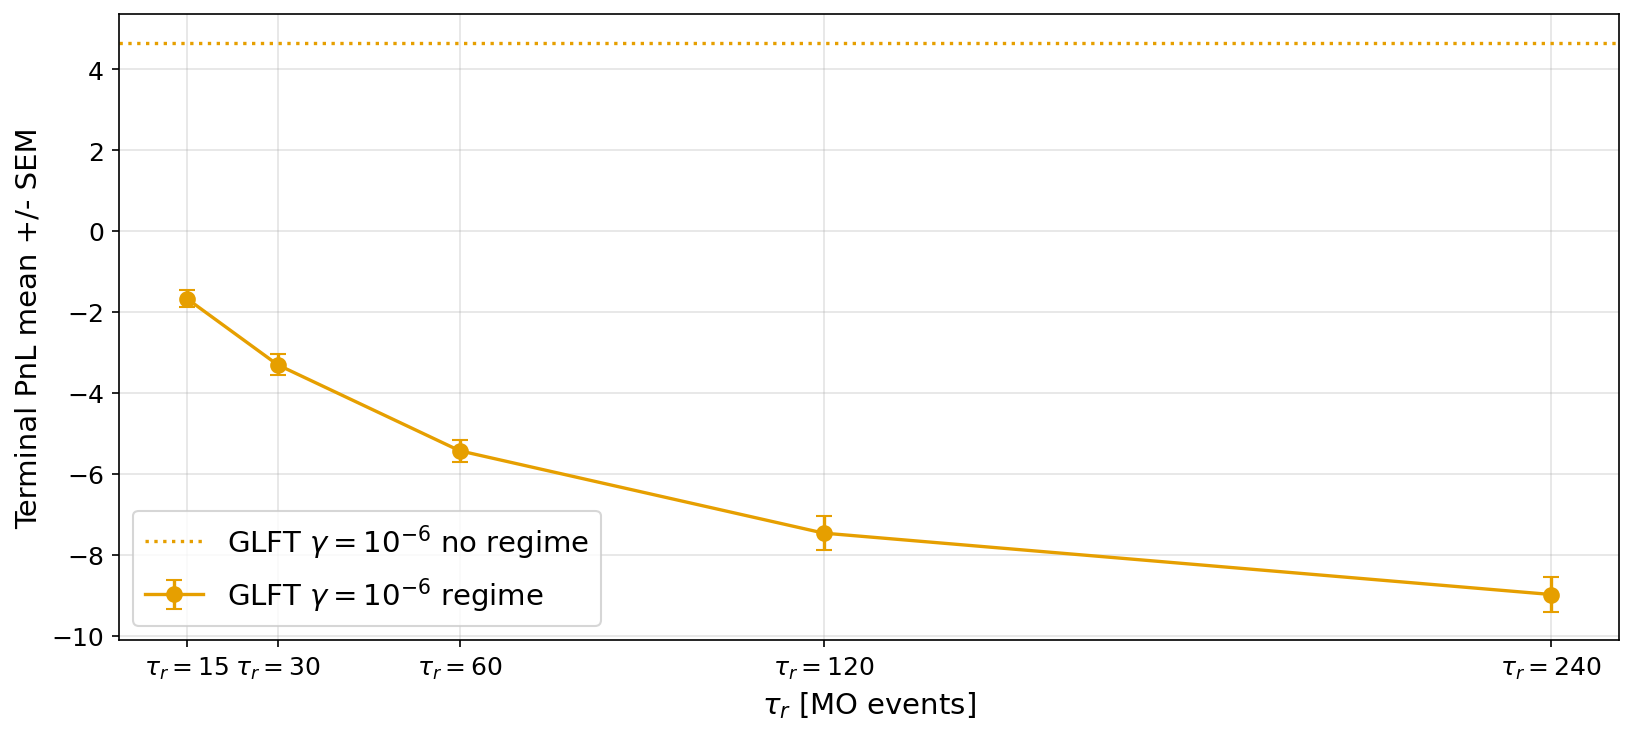
\includegraphics[width=0.7\linewidth]{glft_degradation_vs_tau_regime.png}
  \caption{GLFT mean terminal PnL (with standard errors) under persistent directional regimes as
  a function of the mean regime duration $\tau_r$ (MO clock): the
  buy-MO probability is constant within each regime and regime
  durations are exponentially distributed with mean $\tau_r$ MO
  events, at regime width $\omega = 0.30$ (generative model in
  Section~\ref{sec:robustness}).  The
  dotted line indicates the no-regime baseline.
  }
  \label{fig:glft_degradation_tau}
\end{figure}

\section{Reinforcement Learning Formulation}
\label{sec:learning_formulation}
In this section, we cast the market-making problem as a
reinforcement-learning problem and present the RL solutions we
compare with the GLFT benchmark of
Section~\ref{sec:problem_setup}.  Although the simulator is
event-driven, control is posed at the level of MM decisions rather
than raw book events.  At each decision step the agent observes a
compact decision-time state \(s_t\) (defined in
Eq.~(\ref{eq:state_vector}) below), chooses a discrete quoting
action, lets exogenous order flow evolve, and collects the realized
reward at the next decision step.  The state \(s_t\) retains only the
part of the book directly relevant to quoting---touch spread,
near-touch depths, inventory, and resting-order indicators---and is
treated as the MDP state in the Bellman equations below.  Although the
simulator is Markov in its full book-and-agent state, we train the
MM on this compact \(s_t\).  Under the regime-switching flow
of Section~\ref{sec:robustness} the latent MO-flow regime makes $s_t$
alone non-Markov; Section~\ref{sec:nonstat_training} restores
approximate Markovianity by augmenting $s_t$ with the Bayesian regime
belief $b_t$ of Eq.~\eqref{eq:phaseb_belief_summary}.

\paragraph{Decision clock (throttle).}
The MM does not re-evaluate its quotes on every book event.
Instead, a \emph{time throttle}\footnote{The subscript $c$ stands
for ``controller clock'', distinguishing it from the regime memory
scale $\tau_r$ used later in
Section~\ref{sec:nonstat_training}} $\tau_c$  defines the decision grid in
the \emph{simulated physical time} of the LOB: a new decision is
allowed only when the simulator clock has advanced by at least
$\tau_c$ seconds since the last decision. From now on, in the
reinforcement-learning setting, we use discrete time
$t\in {\mathbb N}$, which advances by one unit at each decision,
i.e., approximately every $\tau_c$ simulated seconds.  In our experiments, we
fix $\tau_c = 1$~simulated second, large enough that typical queue
dynamics play out between decisions (so that rewards are not
dominated by single-event noise) but small enough that the agent
can react to persistent flow imbalances within a few decisions.  With
the calibrated rates of Section~\ref{sec:problem_setup}, the per-second
event counts implied by the simulator are approximately 3.0/s LO
arrivals, 0.2/s MO arrivals and 2.8/s cancellations (the cancellation
rate is fixed by the steady-state balance LO~$=$~MO~$+$~cancellations),
so on average $\bar N_t \approx 6$ book events fall between two
consecutive decisions.
The throttle is a modeling choice rather than a learned object;
its role is to separate the fine-grained book dynamics from the
coarser quoting decisions of the MM.  Two clocks therefore coexist:
the underlying \emph{event clock} on which the book evolves
(continuous-time Markov), and the \emph{decision clock} induced by
the throttle on which the MM observes, acts, and learns.
Between two consecutive decision times the simulator processes a random
number $N_t \ge 1$ of intermediate book events, indexed by
$n = 0, 1, \ldots, N_t-1$ within decision interval~$t$, each
producing a reward $r_{t,n}$ (mark-to-market plus realized
cash flows).  Since $N_t$ varies
across decisions, a fixed one-step discount would weigh decisions
with many or few intermediate events inconsistently.  To keep the
Bellman target on the same event-clock scale regardless of how many
book events fall in a decision interval,
we use the discounted sum of the intermediate per-event rewards,
\begin{equation}
  r_t \;=\; \sum_{n=0}^{N_t-1} \gamma^{n}\, r_{t,n},
  \label{eq:smdp_reward}
\end{equation}
where each per-event reward $r_{t,n}$ is discounted by its offset $n$
from the start of the interval.  The next decision state $s_{t+1}$ is
reached at event offset $N_t$, so under the same event-clock
$\gamma$-discounting its bootstrapped value carries the next factor in
the sequence, $\gamma^{N_t}$.  Because the inter-decision count $N_t$ is
random, the decision-grid process is a \emph{semi-Markov decision
process} (SMDP)~\citep{puterman1994,sutton1999options}, with one-step
target $r_t + \gamma^{N_t}\max_{a'}Q(s_{t+1},a')$.  The factor
$\gamma^{N_t}$ is an effective per-decision discount replacing the fixed
$\gamma$ of a standard MDP; we denote it $\Gamma_t$ below.  When
$N_t \equiv 1$ (no throttling), the sum collapses to $r_t = r_{t,0}$ and
$\Gamma_t=\gamma$, recovering the usual one-step target.  We discount on
the event clock rather than in physical seconds: per-decision payoffs
accrue at discrete book events, and the throttle $\tau_c$ already
controls how much physical time elapses per decision.

\paragraph{State, action, reward.}
The MM operates on the state vector
\begin{equation}
  s_t=
  \bigl[\mathrm{spr}_t,\;
  d_{t,0}^{b},\ldots,d_{t,K}^{b},\;
  d_{t,0}^{a},\ldots,d_{t,K}^{a},\;
  q_t,\;e_t\bigr],
  \label{eq:state_vector}
\end{equation}
where $\mathrm{spr}_t$ is the market bid--ask spread;
$d_{t,k}^{b}$ and $d_{t,k}^{a}$ are the queue depths at offset~$k$
from the best bid and best ask respectively, for $k = 0,\ldots,K$
(with $K=1$ in all reported experiments),
with $d_{t,k}^{b}=d_{t,k}^{a}=0$ when the corresponding level is empty
(so the agent observes the depth profile at every price level where it
can place orders, including empty ones); $q_t$ is the signed inventory; and
$e_t$ is an auxiliary order-flow feature vector used only in the
non-stationary experiments of Section~\ref{sec:robustness}.  The
simulator also tracks whether the MM currently has a live bid or ask
order.  These live-order indicators are used internally to maintain
order persistence, queue priority, inventory gating, and logging. In the stationary experiments of
Section~\ref{sec:stationary_results}, the auxiliary feature vector is switched
off.  In the regime-switching experiments of
Section~\ref{sec:nonstat_training}, the latent directional bias of the
MO flow becomes a hidden state: the agent then needs an inference
signal for the market's current direction and an awareness of its own
exposure to that direction.  To this end, $e_t$ contains two
complementary signals, defined here for completeness and used from
Algorithm~B onwards.

The first signal is a Bayesian online change-point filter~\citep{adams2007bocpd} applied to
the signed market-order stream.  At each MO arrival the filter
updates a posterior over the latent buy-MO probability and the
current run length of the regime.  The MM does not observe
the latent schedule $p_{\mathrm{buy}}(t)$, but it receives only a compact
belief summary,
\begin{equation}
  b_t = \bigl(\widehat{\iota}_t,\;\bar{\ell}_t\bigr),
  \label{eq:phaseb_belief_summary}
\end{equation}
where $\widehat{\iota}_t$ is the posterior estimate of the directional
flow bias, defined as $\widehat{\iota}_t = 2\widehat p_t - 1$ with
$\widehat p_t$ the posterior mean buy-MO probability, and
$\bar{\ell}_t$ is the posterior expected run length. The Bayesian
recursion that produces this belief summary is derived in
Appendix~\ref{app:bayesian_flow_filter}.  The Bayesian filter advances asynchronously on the MO event clock
(one update per market-order arrival), while the MM acts on the
throttle clock with $\tau_c = 1$~s.  At each decision time $t$, the
MM reads the latest belief $b_t$ available --- i.e., the one
produced by the most recent market order to arrive within the past
$\tau_c$, or the value carried over from $t-1$ if no MO arrived in
that interval.

The second signal is endogenous to the market maker's own quotes.  In
our implementation, the agent keeps at most one resting bid and
one resting ask, and each order is a unit lot.  A resting order creates
fill exposure only to the extent that it is alive and has little queue
ahead of it.  Let $\mathrm{qa}_t^b$ and $\mathrm{qa}_t^a$ denote the
number of resting units ahead of the MM's current bid and ask in the
FIFO queues, when those orders are alive; if a side is absent, its
indicator below is zero and the queue-ahead value is immaterial.  We
therefore define the side-specific quote opportunities as
\begin{equation}
  O_t^{b}=
  \frac{\mathbf 1_{\{\text{bid alive}\}}}{1+\mathrm{qa}_t^b},
  \qquad
  O_t^{a}=
  \frac{\mathbf 1_{\{\text{ask alive}\}}}{1+\mathrm{qa}_t^a},
\end{equation}
and define the quote-exposure imbalance seen by the MM as
\begin{equation}
  x_t
  =
  \frac{O_t^{b}-O_t^{a}}{1+O_t^{b}+O_t^{a}}.
  \label{eq:quote_exposure_imbalance}
\end{equation}

Operationally, under unit quotes this feature lies in
$[-1/2,1/2]$: it is $+1/2$ when only a front-of-queue bid is alive,
$-1/2$ when only a front-of-queue ask is alive, and near zero when the
two sides are balanced or both quotes are buried behind long queues.
This signal is deliberately instantaneous rather than a smoothed
fill statistic: it tells the agent whether its current quoting
decision leaves it more exposed to buy- or sell-side market-order
pressure before the next fill is realized.  The auxiliary feature vector is
therefore $e_t=(b_t,x_t)$.

Each action selects a pair of tick offsets $(\Delta_b, \Delta_a)$
relative to the current best quotes.  The resulting bid and ask
prices are
\begin{equation}
  p_t^b = B_t - \Delta_b, \qquad p_t^a = A_t + \Delta_a,
\end{equation}
where $B_t$ is the best bid and $A_t$ is the best ask observed by
the agent at decision time~$t$.  The offset $\Delta_b = 0$ posts
the bid at the current best bid, joining the back of the FIFO
queue at that price level; $\Delta_b > 0$ places it one or more
ticks deeper in the book, reducing fill probability but increasing
the captured spread per fill; and $\Delta_b = -1$ posts it one
tick inside the spread, creating a new best bid one tick above the
previous one and sitting alone at the front of the queue at that
new price level.  The ask offset $\Delta_a$
operates symmetrically.  Each action therefore controls both the
\emph{width} of the quoted spread ($\Delta_b + \Delta_a +
\mathrm{spr}_t$) and its \emph{asymmetry} ($\Delta_a - \Delta_b$),
which functions as an implicit inventory skew. The agent can quote
tighter on the side where it wants to accumulate fills and wider on
the side where it wants to reduce exposure.

In the experiments reported below we restrict the action space to the
six-element vector
\begin{equation}
  \mathcal{A} = \bigl\{
    (-1,-1),\,(-1,0),\,(0,-1),\,(0,0),\,(0,+1),\,(+1,0)
  \bigr\}.
\end{equation}
Three of these actions ($(-1,-1)$, $(-1,0)$,
$(0,-1)$) place at least one quote one tick inside the prevailing
spread, in which case the MM's quote becomes the new best bid or
ask and the spread observed by the rest of the simulated market
narrows by one tick.

We keep the action set deliberately compact: it is the one-tick grid
$\{-1,0,+1\}^2$ with the three economically extreme cells removed---the
two-sided widening $(+1,+1)$, which steps out of both sides at once (a
role we reserve for the inventory-gating layer described below), and
the two-tick skews $(+1,-1)$ and $(-1,+1)$, whose one-tick retreat leg
is unlikely to fill within a $\tau_c = 1$~s epoch and forfeits the FIFO
priority accrued on that side.  The six retained actions still span
quoted widths from $\mathrm{spr}_t-2$ to $\mathrm{spr}_t+1$ ticks and
one-tick skews $\Delta_a-\Delta_b\in\{-1,0,+1\}$, and stronger effective
skews remain reachable dynamically by holding a one-sided action over
consecutive decision epochs.  A smaller action space has fewer
action-conditioned return distributions to fit and concentrates
exploration on economically distinct alternatives, which aids
convergence---most visibly under the non-stationary fine-tuning of
Algorithm~B (ablation below).

\paragraph{Action-space ablation.}
Retraining with the full nine-action grid under otherwise identical
conditions---same seeds, network, reward, and warm-start, so the two
arms differ only in the action set---confirms this.  Under stationary
flow, where the training budget is ample, both grids converge to the
same performance (mean terminal PnL $+0.339$ vs.\ $+0.331$ over
$N_{\mathrm{sim}}=300$ paired episodes, within one standard error; the
three extra cells are selected only $10.3\%$ of the time).  Under the
shorter, non-stationary fine-tuning of Algorithm~B, however, the
six-action controller converges markedly better, dominating the
nine-action grid at every checkpoint over the $4000$ fine-tuning
episodes (best training terminal-PnL moving average $+0.097$ vs.\
$-0.005$).  Fewer actions thus make little difference when data is
plentiful, but converge substantially better under the limited-budget,
non-stationary fine-tuning that matters for robustness.


At each throttle-triggered decision, the agent selects one such
action, and the quotes remain resting in the book until the
next decision epoch, i.e.\ until the simulator clock has advanced
by at least $\tau_c = 1$~simulated second.  The inequality (rather
than equality) reflects the event-driven nature of the simulator: the
throttle gate is evaluated only when the next LOB event (arrival or
cancel) is processed, and the first such event after
$t_{\text{last}} + \tau_c$ generally lands a small random offset past
that boundary.  A safety layer enforces $p_t^b < p_t^a$ to prevent self-crossing.
This only binds when the agent selects $(-1,-1)$ while the observed
spread is at most 2 ticks (with $\mathrm{spr}_t = 1$ the two quotes
would cross, with $\mathrm{spr}_t = 2$ they would coincide); in our
simulations such a configuration occurs in approximately 8\% of
decisions, so the clamp is rarely active.  More importantly, the same
layer enforces the hard inventory bound.  The action set $\mathcal{A}$
is \emph{not} restricted: the policy still selects from the full
six-element grid.  After selection, a post-hoc projection is applied;
when $q_t = +q_{\max}$, the bid leg of the chosen
$(\Delta_b,\Delta_a)$ is dropped while the ask leg is still posted as
proposed, so no additional fills can push the inventory further long;
symmetrically when $q_t = -q_{\max}$, the ask leg is dropped.  The
reward and next state are computed on the post-gating quote, so the
network learns the consequences of the projection rather than
choosing over a state-dependent action set, and the hard bound
$|q_t| \le q_{\max}$ is never violated regardless of the learned
quoting policy.

A second piece of bookkeeping concerns how quotes are managed across
decision steps.  The MM's resting orders persist between decisions.
At each new decision, the MM compares the target price on each
side with the existing resting order: if they match, the order is left
in place and keeps its FIFO position; if they differ, it is canceled
and reposted at the new price (returning to the back of that queue).
This smart-quoting layer is essential: canceling and reposting at the
\emph{same} price every decision would reset queue priority under
price--time priority and erase the spread-capture edge, so queue
priority is treated as an economic resource the agent earns by
holding.

The reward\footnote{We index rewards by the decision time at which
the action is taken: $r_t$ is the reward of the transition
$(s_t,a_t,s_{t+1})$, accrued over the interval $(t,t+1]$ and hence
only observable at time $t+1$.  This transition-indexed convention,
standard in the deep $Q$-learning literature \citep{mnih2015}, is
equivalent to the $R_{t+1}$ indexing of \citet{suttonbarto2018}; we
keep the single index $t$ so that the transition tuple
$(s_t,a_t,r_t,s_{t+1},N_t)$ and the $n$-step sums below carry one
time index per decision.} is a dampened fill PnL---each newly
executed quantity is revalued immediately against the post-decision
mid-price, minus a quadratic inventory penalty augmented by what we
refer to as an inventory-\emph{wall} term---a one-sided quadratic
soft-barrier penalty, in the spirit of penalty methods for
constrained optimization---that activates only beyond a soft
threshold $q_w \in (0, q_{\max})$,
\begin{equation}
  \label{eq:reward}
  r_t
  =
  \sum_{f\in\mathcal{F}_t}
  \Delta q(f)\bigl(m_{t+1}-p(f)\bigr)
  \;-\;
  \varphi\, q_{t+1}^{2}
  \;-\;
  \varphi\bigl(|q_{t+1}|-q_{w}\bigr)_{+}^{2}.
\end{equation}
Here \(\mathcal{F}_t\) is the set of fills received between decision
times \(t\) and \(t+1\); since the MM keeps at most one resting
unit-lot order per side and a filled quote is not replenished until
the next decision epoch, \(\mathcal{F}_t\) contains at most one fill
per side, so \(|\mathcal{F}_t|\le 2\).
Further, \(m_{t+1}\) is the post-action mid-price,
\(p(f)\) is the execution price of fill \(f\),
\(\Delta q(f)\) is the signed executed quantity (positive for
buy-side fills, negative for sell-side fills), \(q_{t+1}\) is the
post-decision inventory, and \(\varphi>0\) controls the risk--return
trade-off between spread capture and inventory containment.  When the
throttle yields $N_t>1$ intermediate events, this per-decision reward
is the offset-weighted sum $\sum_{n=0}^{N_t-1}\gamma^{n} r_{t,n}$ of
Eq.~\eqref{eq:smdp_reward}, each intermediate contribution discounted
by its within-interval offset $n$.  The operator $(u)_{+}=\max(u,0)$ ensures the
wall term is inactive while
\(|q_{t+1}|\le q_{w}\) and grows quadratically once the inventory
exceeds the soft threshold; in our experiments we set
\(q_{w}=q_{\max}/2\), so the wall sharply increases the marginal inventory
penalty over the outer half of the admissible inventory range,
discouraging the policy from drifting close to the hard cap
\(|q_t|\le q_{\max}\) enforced by the unilateral quote-gating layer.
The MM is updated on this decision grid by temporal-difference
learning~\citep{sutton1988td} with discounted bootstrap targets, an
SMDP form of $Q$-learning~\citep{watkins1992qlearning}.  For one transition of
this SMDP, $(s_t,a_t,r_t,s_{t+1},N_t)$, let
$\Gamma_t=\gamma^{N_t}$ denote the effective discount accumulated over
the intervening book events.  The Bellman target is then
$r_t + \Gamma_t\max_{a'}Q_{\theta^-}(s_{t+1}, a')$, where
$\gamma \in (0,1)$ is the per-event discount factor and $\theta^-$
denotes the periodically synchronized target parameters.  Training
minimizes the temporal-difference error between the online
$Q$-estimate $Q_\theta(s_t, a_t)$ and this bootstrapped target.  In the
Double-DQN variant used here~\citep{vanhasselt2016}, action selection
in the target uses the online network while evaluation uses the target
network, giving the one-step (bootstrapped) target $G_t^{(1)}$:
\begin{equation}
  G_t^{(1)}
  =
  r_t+\Gamma_t
  Q_{\theta^-}\!\left(
    s_{t+1},
    \arg\max_{a'} Q_{\theta}(s_{t+1},a')
  \right).
\end{equation}

\paragraph{Rainbow DQN.}
We adopt the Rainbow architecture~\citep{hessel2018} as the learning
backbone for the MM.  Rainbow was chosen for three reasons.  First, it is a
strong value-based default: the combination of orthogonal improvements
reliably outperforms each component alone.  Second, its composable
design enables clean per-component ablation.  Third, and most relevant
here, the distributional C51 branch~\citep{bellemare2017} suits market
making: because execution in a FIFO LOB is inherently uncertain---fills
depend on queue position and stochastic order flow---the per-event
reward is sparse and heavy-tailed, and modeling the full return
distribution rather than just its mean captures the asymmetric PnL
tails that a scalar $Q$-value cannot represent faithfully.

Concretely, the MM combines DQN~\citep{mnih2015}, Double
DQN~\citep{vanhasselt2016}, dueling networks~\citep{wang2016dueling},
prioritized experience replay (PER)~\citep{schaul2016prioritized},
NoisyNet exploration~\citep{fortunato2018noisy}, $n$-step targets,
and C51.
The architecture builds a shared representation
$h_t = \phi_\theta(s_t)$, then splits into a value stream and an
advantage stream, combined as
\begin{equation}
  Q_\theta(s_t,a)
  =
  V_\theta(h_t)
  +
  A_\theta(h_t,a)
  -
  \frac{1}{|\mathcal A|}
  \sum_{a'} A_\theta(h_t,a').
\end{equation}
Here, \(V_\theta(h_t)\) is the estimate of the state-value, 
\(A_\theta(h_t,a)\) is the estimated advantage of action \(a\) relative to the state-value baseline, and
\(|\mathcal A|\) is the number of discrete actions.
To improve data efficiency, replay sampling is prioritized so that
transitions on which the network was most wrong are revisited more
often.  Each transition $i$ in the buffer carries a non-negative
\emph{priority score} $p_i$ set to the magnitude of its last
training error---in our distributional (C51) MM, the
categorical cross-entropy between the projected target and the
predicted return distributions, the distributional analogue of the
absolute TD-error---and refreshed whenever the
transition is replayed.  The next sample is then drawn with
probability
\begin{equation}
  P(i)=
  \frac{(p_i+\varepsilon_{0})^\alpha}
       {\sum_j (p_j+\varepsilon_{0})^\alpha},
  \qquad
  w_i \propto \bigl(|\mathcal B|P(i)\bigr)^{-\beta},
\end{equation}
where $\varepsilon_{0}>0$ prevents zero-probability sampling of
transitions whose last error was exactly zero,
$\alpha \in [0,1]$ interpolates between uniform replay
($\alpha=0$) and fully proportional sampling ($\alpha=1$),
$|\mathcal B|$ is the replay-buffer size, and the
importance-sampling weight $w_i$ re-weights each gradient update
to compensate for the non-uniform sampling, with
$\beta \in [0,1]$ controlling how aggressively that correction is
applied (so the expected loss converges to its uniform-replay
counterpart as $\beta \to 1$).  Exploration is handled by
NoisyLinear layers,
\begin{equation}
  y=
  (\mu^W+\sigma^W\odot\varepsilon^W)x
  +
  (\mu^b+\sigma^b\odot\varepsilon^b),
\end{equation}
while C51 predicts a categorical return distribution instead of
only a scalar \(Q(s,a)\).  Concretely, the network outputs, for
every state--action pair, a probability mass function over a fixed
support of $N$ values (called \emph{atoms}) that covers the
plausible range of cumulative returns; the scalar $Q$-value is then
recovered as the expected return under that distribution.  Atom
locations and the implied $Q$-value are
\begin{equation}
  z_i = V_{\min} + (i-1)\Delta z,
  \qquad
  Q(s,a)=\sum_{i=1}^{N} z_i\,\pi_i(s,a).
\end{equation}
Here \(\pi_i(s,a)\in[0,1]\) is the probability mass that the C51 head
assigns to atom \(z_i\) for action \(a\) in state \(s\), with
\(\sum_{i=1}^{N}\pi_i(s,a)=1\).  Thus \(Q(s,a)\) is the mean of the
predicted categorical return distribution.
In the NoisyLinear layer, \(\mu^W,\mu^b\) are deterministic weights and
biases, \(\sigma^W,\sigma^b\) are learned noise scales,
\(\varepsilon^W,\varepsilon^b\) are random perturbations, and \(\odot\)
denotes element-wise multiplication.  In the C51 representation,
\(V_{\min}\) and \(V_{\max}\) define the lower and upper ends of
the fixed return support, \(z_i\) is atom \(i\) on a support of
size \(N=101\) in the experiments reported here,
\(\Delta z=(V_{\max}-V_{\min})/(N-1)\).
The projected target distribution is obtained by applying the
standard $1$-step Bellman operator to each atom of the next-state
distribution: each atom $z_i$ is shifted to
$r_t + \Gamma_t\,z_i$ (or, with the $n$-step targets used here, by the $n$-step return defined below), and the resulting probability masses are
re-projected back onto the fixed support $\{z_1,\dots,z_N\}$.
Let \(\pi_i^{\mathrm{target}}(s_t,a_t)\) denote the resulting target
mass assigned to atom \(z_i\).  The network is trained to match this
target distribution by minimizing the categorical cross-entropy loss
\begin{equation}
  \mathcal L_{\mathrm{C51}}
  =
  -
  \sum_{i=1}^{N}
  \pi_i^{\mathrm{target}}(s_t,a_t)\log \pi_i(s_t,a_t).
\end{equation}

To propagate reward information faster across the decision grid,
the $1$-step bootstrap above is replaced by an $n$-step return~\citep{suttonbarto2018}
that chains $n$ consecutive decision-level rewards
$r_t, r_{t+1}, \ldots, r_{t+n-1}$, defined as in
Equation~\eqref{eq:smdp_reward}, before bootstrapping.  Each decision
interval $t+i$ spans $N_{t+i}$ book events, so the per-decision
discount is $\gamma^{N_{t+i}}$ rather than a fixed $\gamma$.  The
cumulative discount from the root decision $t$ to the start of
decision $t+i$ is then
\begin{equation}
  M_i \;=\; \sum_{j=0}^{i-1} N_{t+j},
  \qquad M_0 = 0,
\end{equation}
i.e.\ the total number of micro-step events elapsed.  The $n$-step
target generalizes the one-step target $G_t^{(1)}$ above:
\begin{equation}
  G_t^{(n)}
  \;=\;
  \sum_{i=0}^{n-1} \gamma^{M_i}\, r_{t+i}
  \;+\;
  \gamma^{M_n}\,
  Q_{\theta^-}\!\bigl(s_{t+n},\,\arg\max_{a'} Q_\theta(s_{t+n},a')\bigr).
\end{equation}
As in the single-step case, $M_i = i$ when $N_{t+j}\equiv 1$ for all $j<i$, so
$G_t^{(n)}$ recovers the standard $n$-step DQN target; under throttle,
the random-duration discounting keeps the per-decision discount factors consistent with
the event clock.  Larger $n \ge 1$ propagates reward information
further, reducing the one-step bootstrap bias at the cost of higher
variance in the value targets.

The main architectural and optimization hyperparameters of the neural
MM are summarized in Table~\ref{tab:dqn_hyperparams}.

\begin{table}[t]
  \centering
  \caption{Main neural-MM hyperparameters used in the reported
  DQN experiments.}
  \label{tab:dqn_hyperparams}
  \begin{tabular}{p{0.32\linewidth}p{0.58\linewidth}}
    \toprule
    Component & Setting \\
    \midrule
    Feature trunk & One hidden layer with 256 units \\
    Activation & ReLU \\
    Value/action head & Dueling C51 head over six quote-offset actions;
      101 atoms on the support $[-3,3]$ \\
    Discount and TD horizon & Per-event discount $\gamma=1-10^{-3}$;
      $n=3$ decision-level SMDP targets \\
    Optimization and replay & AdamW with initial learning rate
      $3\times 10^{-4}$; batch size 64; prioritized replay buffer
      of size $10^5$; target-network update every 2000 gradient steps \\
    \bottomrule
  \end{tabular}
\end{table}


\FloatBarrier
\section{Stationary Order Flow Results}
\label{sec:stationary_results}

We report the performance of the trained Rainbow DQN under
stationary and symmetric order flow against the calibrated GLFT
benchmark and the at-best baseline.  All results use paired-seed
evaluation episodes (same exogenous flow realizations across
policies), and training and evaluation episodes are strictly
disjoint.

\begin{figure}[htbp]
  \centering
  \begin{subfigure}[b]{0.49\linewidth}
    \centering
    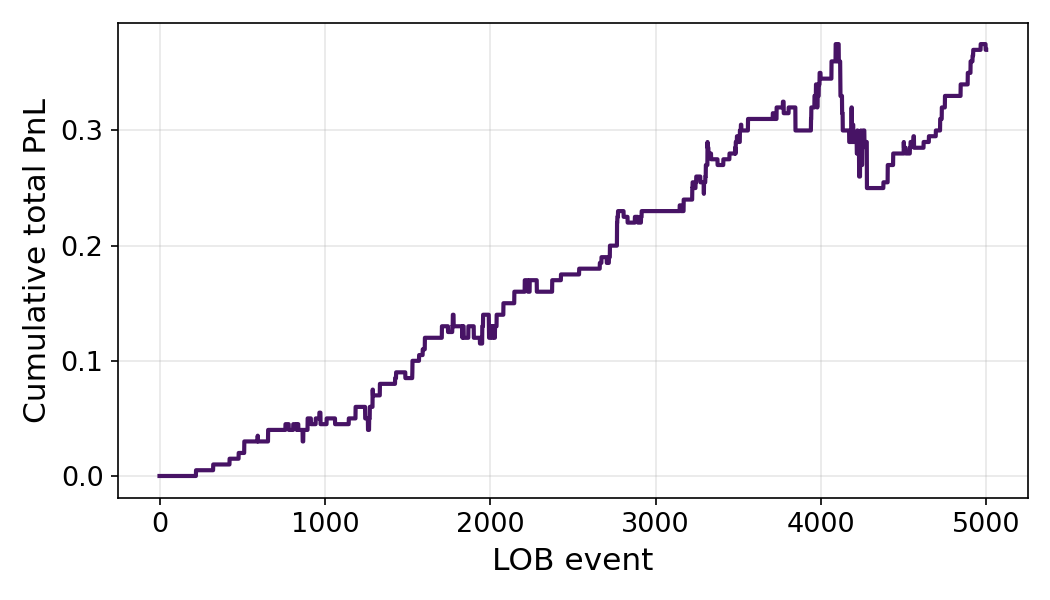
\includegraphics[width=\linewidth]{total_pnl_0001.png}
    \caption{Cumulative total PnL.}
    \label{fig:dqn_pnl}
  \end{subfigure}
  \hfill
  \begin{subfigure}[b]{0.49\linewidth}
    \centering
    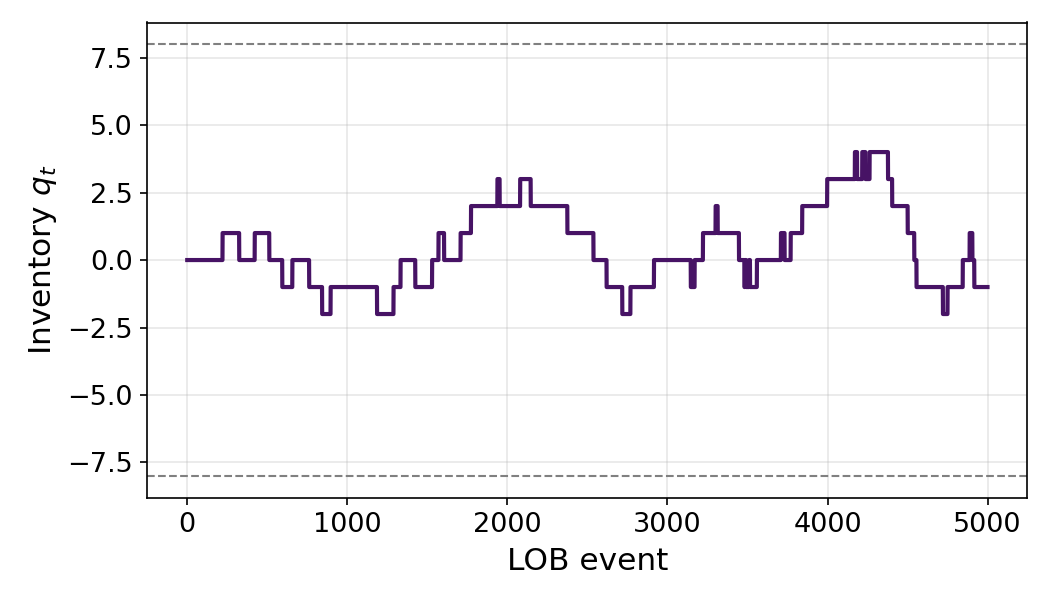
\includegraphics[width=\linewidth]{MM_inv_0001.png}
    \caption{Inventory trajectory.}
    \label{fig:dqn_inv}
  \end{subfigure}
  \caption{Representative episode of the trained Rainbow DQN under
  stationary and symmetric market order flow (inventory penalty $\varphi = 10^{-3}$, hard
  inventory bound $q_{\max} = 8$).  (\subref{fig:dqn_pnl})
  Positive and steadily growing cumulative PnL accumulated through
  passive spread capture.  (\subref{fig:dqn_inv}) Inventory
  trajectory: the quadratic penalty $\varphi q^2$ keeps excursions
  bounded within $\pm q_{\max}$, with frequent mean-reversion
  toward zero.}
  \label{fig:dqn_episode}
\end{figure}

Figure~\ref{fig:dqn_episode} shows a representative trained
episode: the agent accumulates positive PnL through passive fills
(panel~\subref{fig:dqn_pnl}) while inventory mean-reverts within
the $\pm q_{\max}$ corridor (panel~\subref{fig:dqn_inv}),
confirming that the policy is genuine spread-capture market
making rather than directional trading.

Comparing the performance of GLFT and Rainbow DQN requires a matching of the risk aversion parameter of the former with the inventory penalty of the latter. Since the mapping is not evident, we run simulations for both models under different values of these parameters and then compare the results in a return-risk plane. Figure~\ref{fig:dqn_frontier} shows the results over
$N_{\mathrm{sim}} = 1000$ paired-seed evaluation episodes,
sweeping $\gamma_{\mathrm{GLFT}}$ for GLFT (blue) and $\varphi$ for the Rainbow DQN
(orange), with the at-best baseline (gray) as a further comparison.  It is evident that the
DQN frontier lies above the GLFT frontier throughout the observed
risk range, indicating that the reinforcement-learning method finds better strategies than GLFT.

\begin{figure}[htbp]
  \centering
  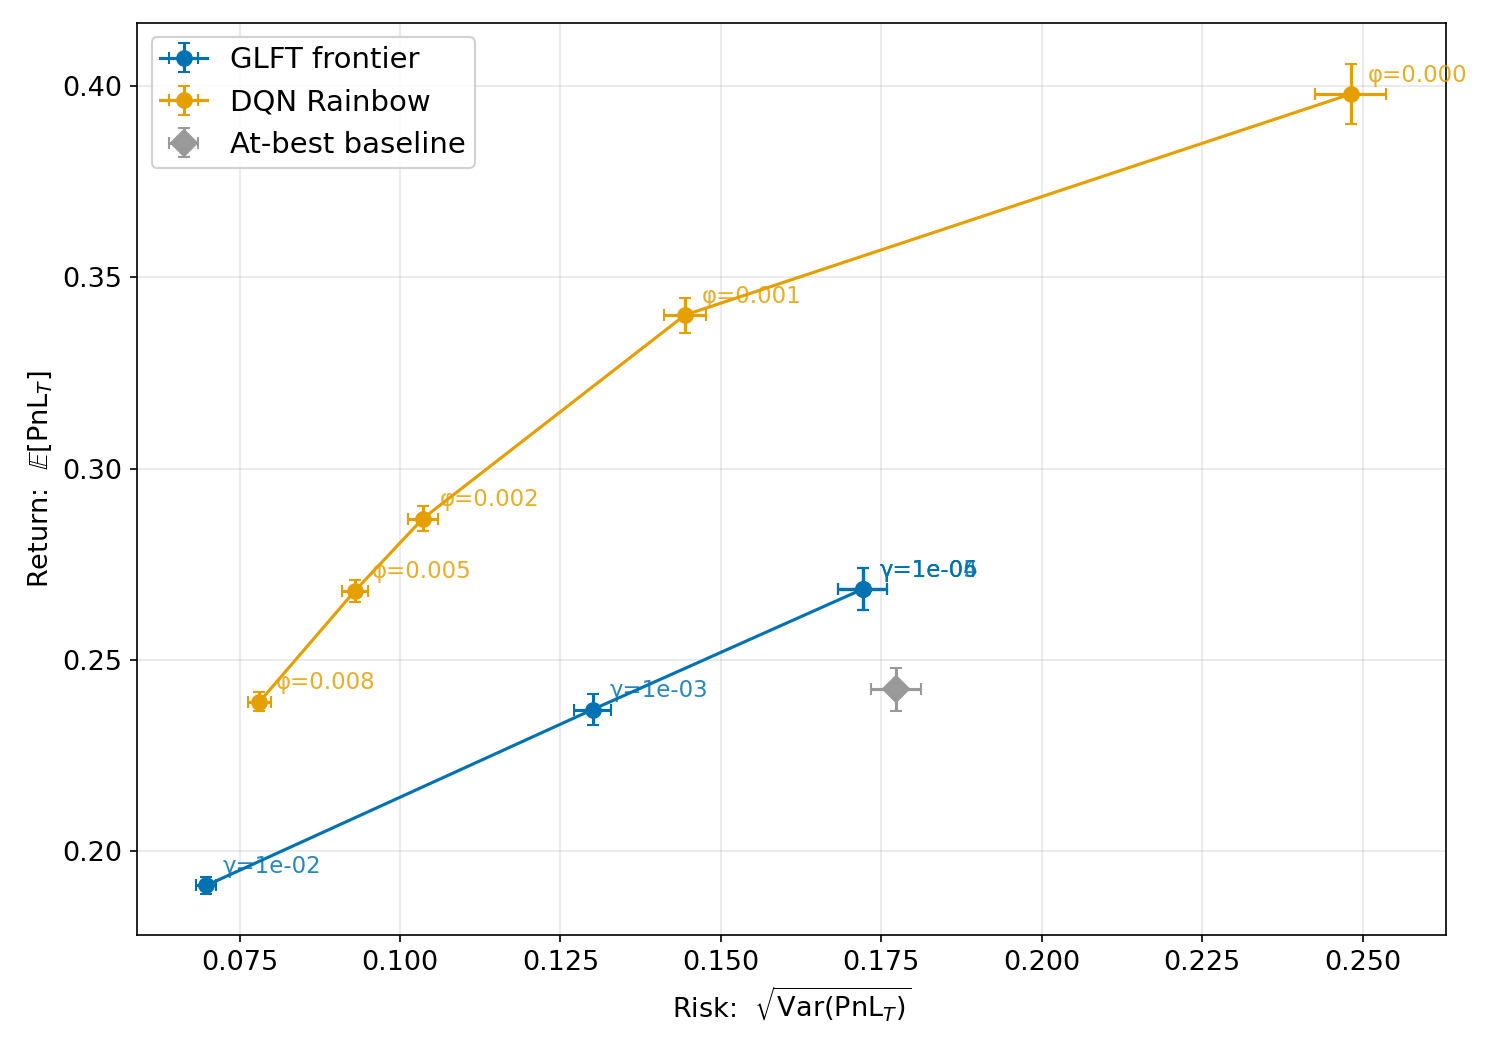
\includegraphics[width=0.7\linewidth]{glft_frontier_complete.png}
  \caption{Risk--return efficient frontier over
  $N_{\mathrm{sim}} = 1000$ paired-seed evaluation episodes: the
  GLFT curve (blue) sweeps $\gamma_{\mathrm{GLFT}}$, the Rainbow DQN curve (orange)
  sweeps $\varphi$, and the at-best baseline (gray) serves as
  a reference point.  Each marker is labeled by its swept
  parameter value.}
  \label{fig:dqn_frontier}
\end{figure}

We refer to the policy obtained at the end of this stationary
training pipeline as the \emph{Algorithm~A controller}---our
stationary-flow baseline controller---the benchmark for
the non-stationary experiments of Section~\ref{sec:robustness}.

\section{The Robustness Problem}
\label{sec:robustness}

\paragraph{Motivation: from static asymmetry to regimes.}
Section~\ref{sec:problem_setup} documented the empirical failure that
motivates this section: when real MO flow alternates between persistent
buy- and sell-pressure regimes, a modest \emph{static} imbalance
already pushes both GLFT and the stationarily trained learner toward
losses (Figure~\ref{fig:misspec_comparison}), and under
\emph{persistent} regimes the GLFT PnL collapses monotonically in the
regime persistence (Figure~\ref{fig:glft_degradation_tau}).  It is
therefore essential to test the controller not only in the
stationary market where it was trained, but under counterfactual
non-stationary flow, to separate how much of its stationary edge is
robust from how much is brittle.  This section specifies the regime
model behind those stress tests, dissects the failure mechanism of
the stationarily trained Algorithm~A controller, and thereby sets up the
flow-aware retraining of Section~\ref{sec:nonstat_training}.

\paragraph{Regime generation.}
We model the non-stationary flow as a piecewise-constant process
on $p_{\mathrm{buy}}$, indexed on the \emph{MO clock}: regime
boundaries are placed at MO arrivals, so a regime $k$ ``lasts $L_k$
MO events'' and its physical duration scales inversely with the
MO rate $2\mu$ of Section~\ref{sec:problem_setup}.  Regime
durations are drawn independently from an exponential
distribution,
\begin{equation}
  L_k \sim \mathrm{Exp}(1/\tau_r),
\end{equation}
where $\tau_r > 0$ is the mean regime length in MO events. The
buy-MO probability within regime $k$ is sampled uniformly,
\begin{equation}
  p_{\mathrm{buy},k} \sim \mathrm{Uniform}[0.50 - \omega,\; 0.50 + \omega],
\end{equation}
where the \emph{regime-width parameter} $\omega \in [0,
\omega_{\max}]$ controls the severity of the imbalance.  At
$\omega = 0$ the market simulator reduces to the stationary
case; throughout the non-stationary experiments of this paper we
fix $\omega = 0.30$ so that $p_{\mathrm{buy}} \in [0.20, 0.80]$,
and we let $\tau_r$ be the sole control parameter governing the
\emph{persistence} of the imbalance.  Larger $\tau_r$ means
longer-lived buy- or sell-heavy regimes, hence more sustained
adverse selection against a market maker that does not adapt to
the regime.  The latent schedule $p_{\mathrm{buy}}(t)$ itself is
not observable by the agent, which must therefore infer the
current regime implicitly from the Bayesian flow belief and from its
own quote-exposure state.  Figure~\ref{fig:regime_model} illustrates
the generative model.

\begin{figure}[htbp]
  \centering
  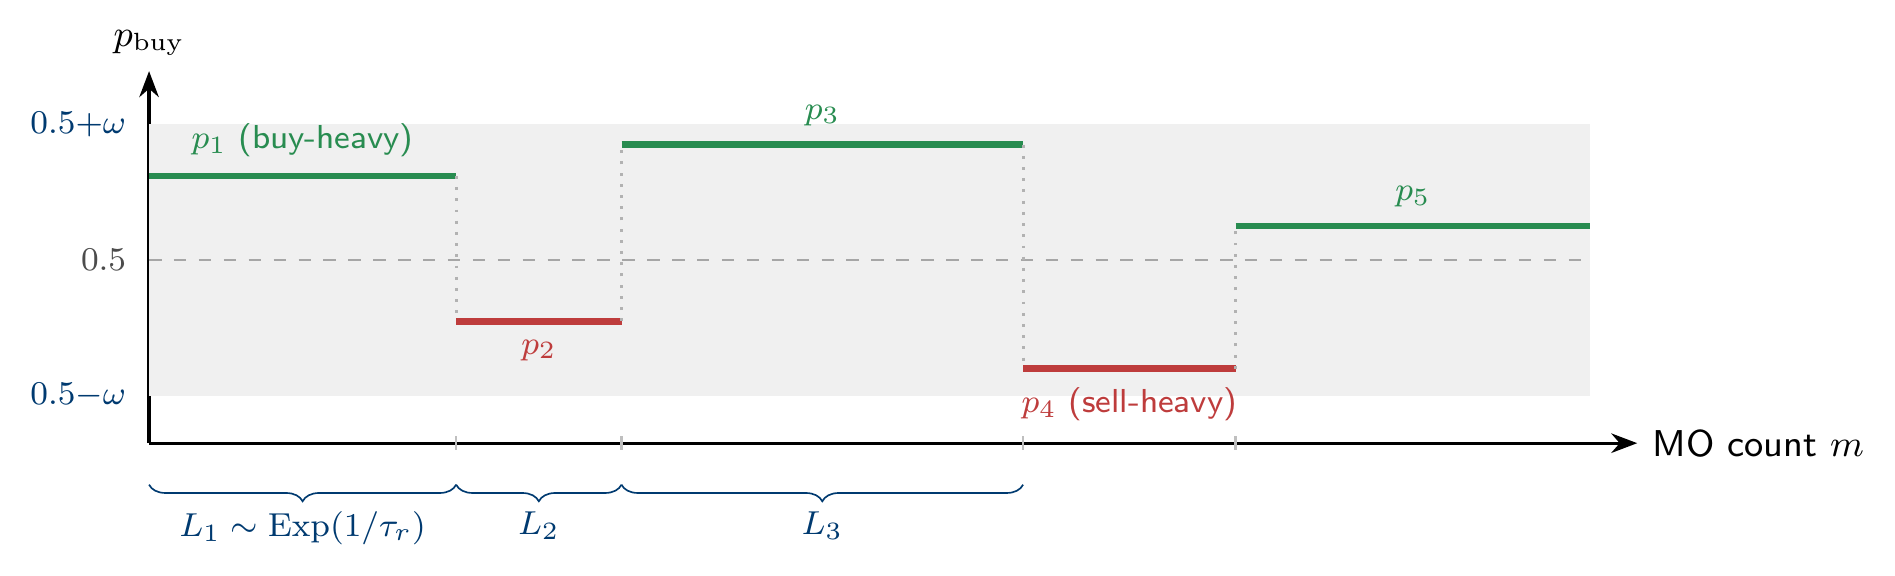
\includegraphics[width=0.85\linewidth]{regime_model_diagram.png}
  \caption{The regime-switching flow model on the MO clock.  Within
  regime $k$ the buy-MO probability is held constant at
  $p_{\mathrm{buy},k} \sim \mathrm{Uniform}[0.50-\omega,\,
  0.50+\omega]$ (green: buy-heavy; red: sell-heavy; shaded band of
  width $2\omega$), and regime durations
  $L_k \sim \mathrm{Exp}(1/\tau_r)$ are drawn on the MO clock.
  Throughout the non-stationary experiments $\omega = 0.30$.}
  \label{fig:regime_model}
\end{figure}

\paragraph{Monte-Carlo comparison at fixed asymmetry.}
We now detail the fixed-asymmetry comparison previewed in
Figure~\ref{fig:misspec_comparison} of
Section~\ref{sec:problem_setup}.  There, the buy-MO probability
$p_{\mathrm{buy}}$ is held constant throughout each episode (so there
is no regime switching and $\tau_r$ plays no role), which isolates the
effect of pure asymmetry before the persistence sweep of
Figure~\ref{fig:degradation_tau} below.  The Rainbow DQN (orange) and
the GLFT policy run inside the LOB simulator (solid blue, ``empirical'')
are evaluated by Monte-Carlo; the dashed blue curve is the closed-form
analytical approximation to the GLFT solution under a misspecified flow.  In short, the GLFT
agent computes its quotes assuming symmetric flow, so under
the true buy-MO probability $p_{\mathrm{buy}}$  the realized ask-side fills come
from the buy-MO flow of intensity $2 p_{\mathrm{buy}}\mu$
and the bid-side fills from the sell-MO flow of intensity
$2(1-p_{\mathrm{buy}})\mu$; the agent realizes only a queue-adjusted fraction of this arrival flow, captured by the effective fill rate $A_{\mathrm{eff}}$ introduced below.

In a realized FIFO LOB the agent shares queues with other resting
orders and can lose priority through the discrete decision clock, so it
captures only a fraction of the ideal GLFT intensity $Ae^{-\kappa\delta}$;
we absorb this into an \emph{effective baseline rate}
$A_{\mathrm{eff}}=\eta A$, with the queue-competition factor
$\eta\approx0.82$ calibrated once offline as the ratio of the measured
to the GLFT-predicted symmetric fill rate.  Under a true buy probability
$p_{\mathrm{buy}}$, the realized ask- and bid-side fill rates pick up
factors $2p_{\mathrm{buy}}$ and $2(1-p_{\mathrm{buy}})$ on this effective
intensity, so the inventory evolves as a bounded birth--death chain
(outward transitions suppressed at the hard cap).  Its stationary law is
a tilted discrete Gaussian and the induced expected-PnL curve admits a
closed form; Appendix~\ref{app:glft_misspecification} gives the
self-contained derivation---the calibration of $\eta$, the stationary
law, the drift-corrected expected PnL, and the diagnostic plots.
The comparison is informative on two counts.  First, the two GLFT
curves are nearly indistinguishable, which validates the
analytical-misspecification approximation as a faithful proxy for the
empirical GLFT policy.  Second, the Rainbow DQN curve sits
\emph{above} both GLFT benchmarks at every level of asymmetry
$|p_{\mathrm{buy}} - 0.50| > 0$, with the gap widening as the flow
becomes more skewed---quantifying the headline of
Section~\ref{sec:problem_setup}: the RLMM remains profitable over
$p_{\mathrm{buy}} \in [\,0.40, 0.60\,]$ while both GLFT variants
cross into losses at $|p_{\mathrm{buy}} - 0.50| \approx 0.08$, so the
learned policy inherits the same structural fragility as any
stationarily trained strategy but operates on a more favorable
envelope.

\paragraph{Single-episode diagnostic.}
The static-asymmetry view of Figure~\ref{fig:misspec_comparison}
isolates directional misspecification but suppresses the temporal
structure of the imbalance.  We therefore zoom into a single
representative episode under genuinely regime-switching flow.
Figure~\ref{fig:regime_episode} illustrates the failure of a
stationarily trained Algorithm~A controller (defined at the end of
Section~\ref{sec:stationary_results}) exposed to this
non-stationary flow.  The top panel shows a realization of the latent
regime schedule, with green regions marking buy-heavy intervals
($p_{\mathrm{buy}} > 0.50$) and red regions marking sell-heavy ones.
The middle panel compares the cumulative PnL of the same Algorithm~A
agent under regime-switching flow (orange) against its behavior under
symmetric baseline flow (gray).  Under balanced flow the agent
steadily accumulates profit, consistent with the stationary results
of Section~\ref{sec:stationary_results}, whereas under regime-switching it
suffers compounding drawdowns during persistent directional regimes. The bottom panel reveals the
mechanism: during sustained buy-heavy or sell-heavy regimes, the
agent's inventory is pushed to the hard inventory limit ($\pm 8$), where it
remains trapped until the regime reverts.  Each such episode of
inventory saturation generates adverse-selection losses that erode
the spread-capture edge.

\begin{figure}[htbp]
  \centering
  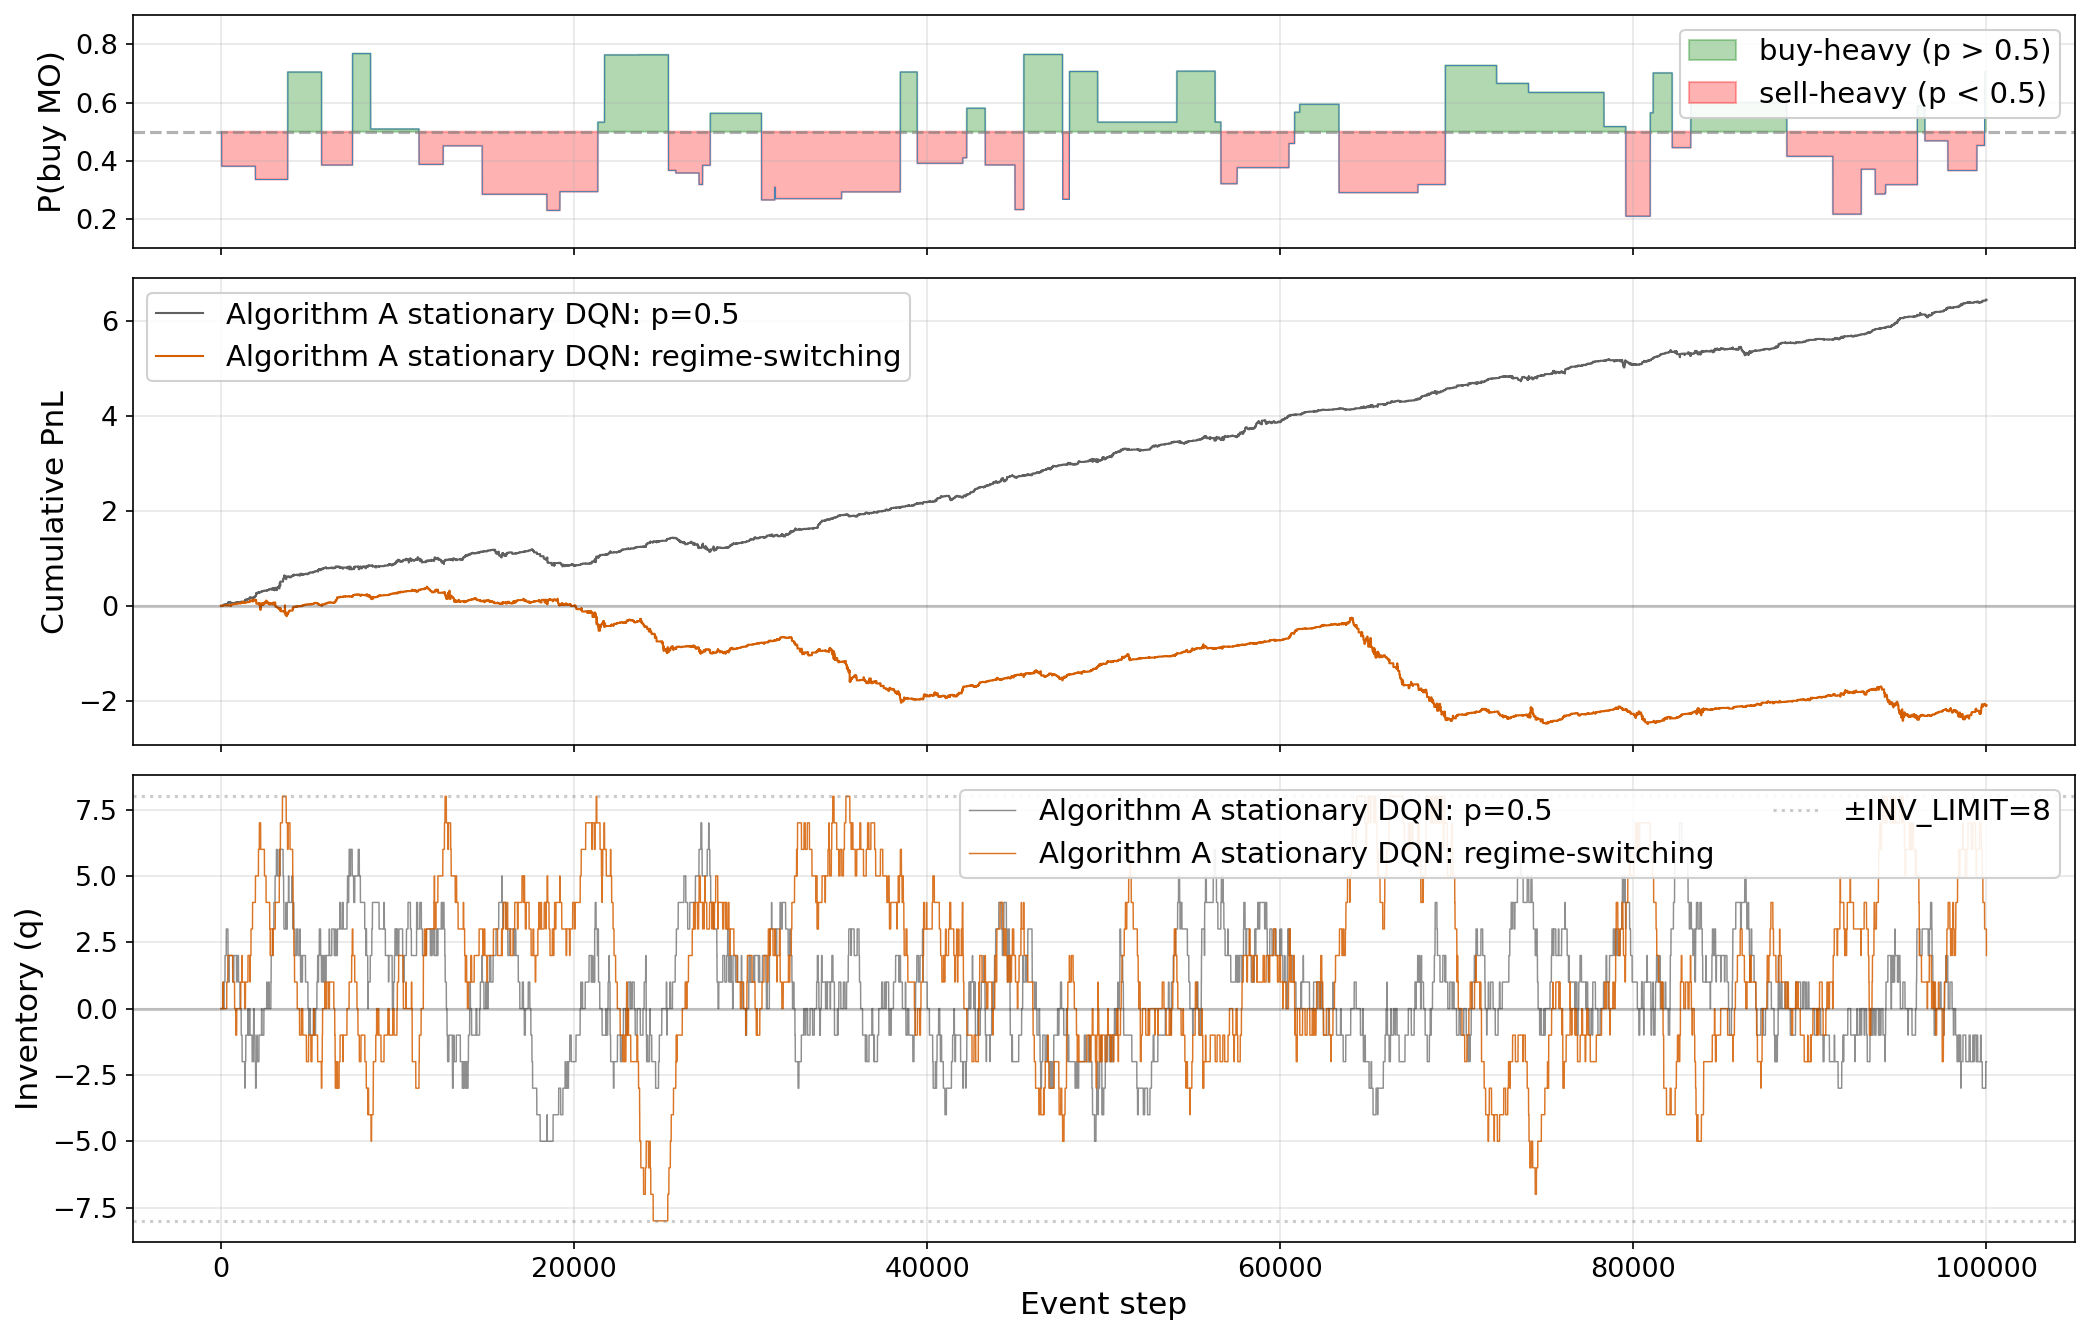
\includegraphics[width=0.8\linewidth]{regime_switching_one_episode_example.png}
  \caption{Single-episode diagnostic under regime-switching flow
  ($\tau_r = 60$ MO events, $\omega = 0.30$; Algorithm~A trained controller with
  inventory penalty $\varphi = 10^{-3}$).
  Top: latent $p_{\mathrm{buy}}$ schedule (green = buy-heavy,
  red = sell-heavy).
  Middle: cumulative PnL under regime-switching (orange) vs.\ symmetric
  baseline (gray).
  Bottom: inventory trajectory; the agent repeatedly hits the
  $\pm 8$ inventory limit during sustained directional regimes.}
  \label{fig:regime_episode}
\end{figure}

\paragraph{Performance degradation as a function of $\tau_r$.}
The single-episode pathology of Figure~\ref{fig:regime_episode}
already suggests that performance degrades systematically as
the directional regimes become more persistent.
Figure~\ref{fig:degradation_tau} reports this central robustness
diagnostic at the population level---the learned-agent counterpart of
the GLFT collapse documented in
Figure~\ref{fig:glft_degradation_tau}---namely the terminal PnL of two
stationarily trained Algorithm~A controllers (inventory penalties
$\varphi = 10^{-3}$ and $\varphi = 5\cdot 10^{-3}$) evaluated over
$N_{\mathrm{sim}} = 100$ paired-seed regime-switching episodes,
sweeping the regime timescale
$\tau_r \in \{15,30,60,120,240\}$ MO events at fixed
$\omega = 0.30$, against a no-regime ($\omega = 0$) baseline.
Both curves are monotonically decreasing in $\tau_r$, exactly
as expected: longer regimes mean more persistent directional
pressure and more compounded adverse-selection losses against
a market maker that does not switch modes with the flow.  The
less risk-averse agent ($\varphi = 10^{-3}$, orange) degrades
more aggressively and eventually becomes loss-making as regimes
become highly persistent; the more risk-averse agent
($\varphi = 5\cdot 10^{-3}$, navy) degrades more slowly, but
still gives up a substantial fraction of its no-regime PnL at
the largest tested persistence scales.  This degradation is not
a marginal effect: for long $\tau_r$, policies that were profitable
in the stationary market are either substantially reduced in
profitability or actively losing.  The motivation for Algorithm~B
is therefore not simply to recover a few percentage points of PnL,
but to prevent this monotone collapse as the order flow becomes
more persistent.

\begin{figure}[htbp]
  \centering
  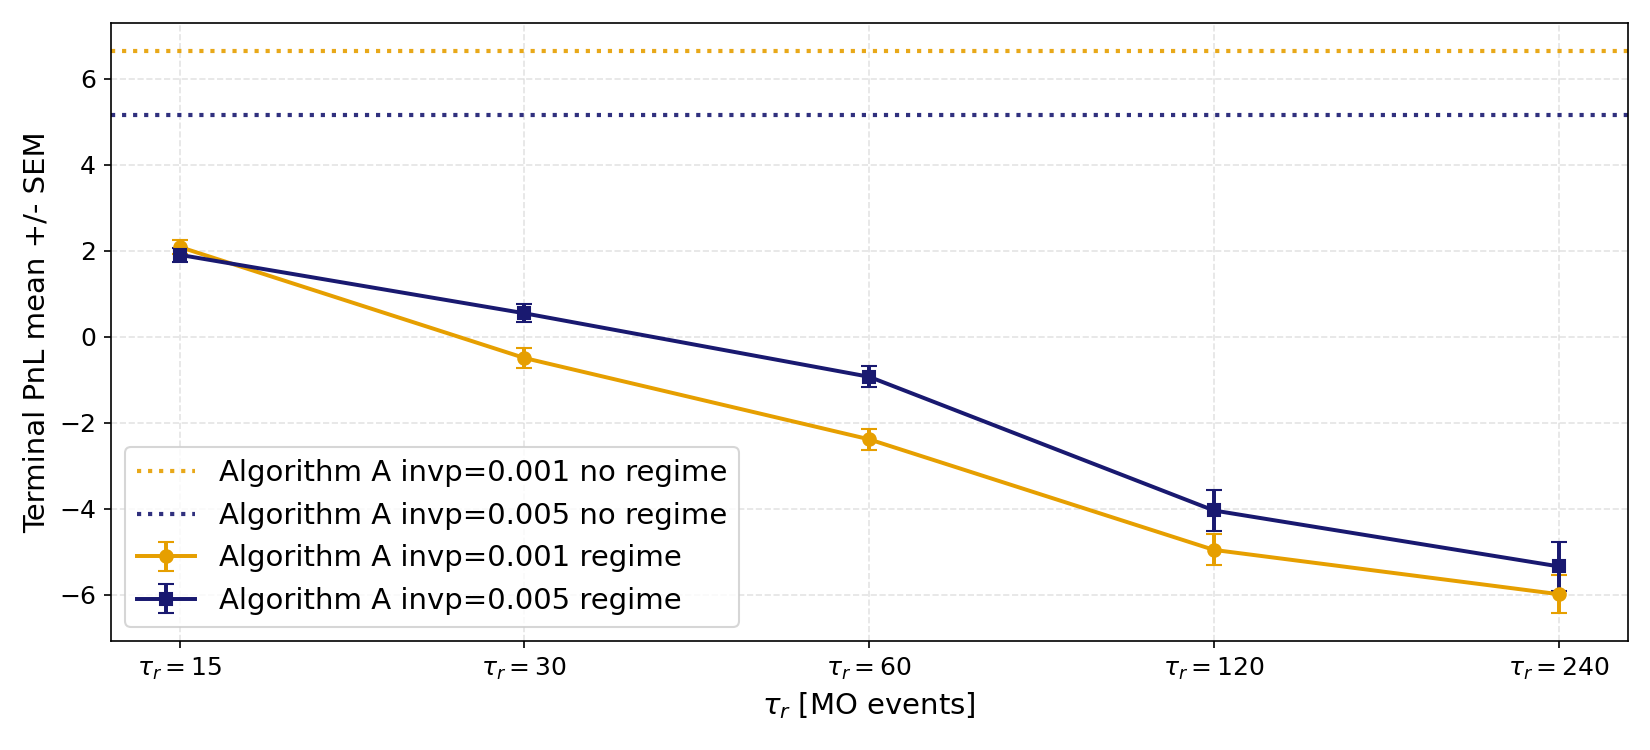
\includegraphics[width=0.7\linewidth]{degradation_vs_tau_regime.png}
  \caption{Terminal-PnL degradation of stationarily trained Algorithm~A
  agents under regime-switching flow vs.\ mean regime duration $\tau_r$
  (MO clock), at fixed width $\omega = 0.30$, over
  $N_{\mathrm{sim}} = 100$ paired-seed episodes.  Mean terminal PnL
  $\pm$ SEM for two inventory penalties ($\varphi = 10^{-3}$, orange;
  $\varphi = 5\cdot 10^{-3}$, navy) over
  $\tau_r \in \{15,30,60,120,240\}$; dotted lines mark the no-regime
  expected PnL baselines.  PnL decreases monotonically in $\tau_r$: longer
  directional regimes generate more adverse selection against a
  non-regime-aware maker.}
  \label{fig:degradation_tau}
\end{figure}

In the remainder of the paper we therefore introduce a Algorithm~B
fine-tuning stage that re-trains the Algorithm~A controller
\emph{directly} on the regime-switching time series defined
above, augmented with a Bayesian change-point representation of
directional flow and a queue-adjusted quote-exposure imbalance.

\section{Training under Non-Stationary Order Flow}
\label{sec:nonstat_training}

Algorithm~B---our regime-aware fine-tuning---improves the
Algorithm~A controller of
Section~\ref{sec:stationary_results} on the regime-switching flow
defined in Section~\ref{sec:robustness}, with the auxiliary feature
vector $e_t=(b_t,x_t)$ of Section~\ref{sec:learning_formulation} now
activated (it was switched off in Algorithm~A).  The purpose is to turn
the stationary spread-capture policy into a controller that can
condition quotes on the partially observed order-flow regime without
changing the action space, reward, or simulator.

\paragraph{MO-clock implementation.}
The simulator advances on the LOB-event clock (every order-book event),
but the regime schedule of Section~\ref{sec:robustness} is defined on
the MO clock (regime durations $L_k$ are counted in market orders).
To pre-generate a single regime schedule per episode --- which keeps
seeding deterministic and decouples the schedule from the policy ---
we therefore need an upper estimate of how many market orders an
episode of $N_{\mathrm{steps}}$ LOB events contains.  Before training,
$E_{\mathrm{calib}} = 5$ passive calibration episodes estimate the
empirical market-order fraction
\[
  \widehat p_{\mathrm{MO}}
  =
  \frac{1}{E_{\mathrm{calib}}}
  \sum_{e=1}^{E_{\mathrm{calib}}}
  \frac{N^{\mathrm{MO}}_e}{N_{\mathrm{steps}}},
\]
where $N^{\mathrm{MO}}_e$ is the number of market orders observed in
the calibration episode $e$.  The expected MO horizon of a training
episode is then
\begin{equation}
  \widehat M
  =
  \left\lceil
    N_{\mathrm{steps}}\,\widehat p_{\mathrm{MO}}
  \right\rceil ,
  \label{eq:mo_horizon}
\end{equation}
and we draw a regime schedule of length $\widehat M$ once, before the
episode starts.  At run time the schedule is advanced and the Bayesian
filter of Appendix~\ref{app:bayesian_flow_filter} is updated only on
market-order arrivals, so both indices equal the running MO count and
the latent regime and the agent's belief over it stay on a common
clock.

\paragraph{Algorithm~B result.}
Figure~\ref{fig:regime_trained} reports a first evaluation of a
Algorithm~B controller trained under regime-switching flow ($\tau_r = 60$
MO events, $\omega = 0.30$) with the auxiliary signals described
above.  The same regime-switching episode is used to compare three
policies: the Algorithm~A baseline under symmetric flow (gray,
reference trajectory), the Algorithm~A controller exposed to
regime-switching without any fine-tuning (orange), and the Algorithm~B
agent under regime-switching (blue); the gray and orange
trajectories are, by construction, the same simulation already
analyzed in Figure~\ref{fig:regime_episode}.  Two observations
emerge.
First, the Algorithm~B controller (blue) recovers a substantial fraction of
the stationary PnL: its cumulative PnL grows steadily and ends, in this single
illustrative episode, at roughly one third of the Algorithm~A symmetric-flow
benchmark---in line with the $37\%$ population figure from the
Monte-Carlo analysis below---with a paired improvement over the
non-adapted Algorithm~A controller of about two thirds of that benchmark
in this episode (about $80\%$ at the population level). Second,
the inventory panel
makes the mechanism explicit: the blue trajectory is markedly
tighter and rarely touches the hard $\pm q_{\max}$ caps, indicating
that the Algorithm~B controller actively skews quotes against the
prevailing regime and prevents the directional accumulation that
drives the losses of the non-adapted Algorithm~A controller.

\begin{figure}[htbp]
  \centering
  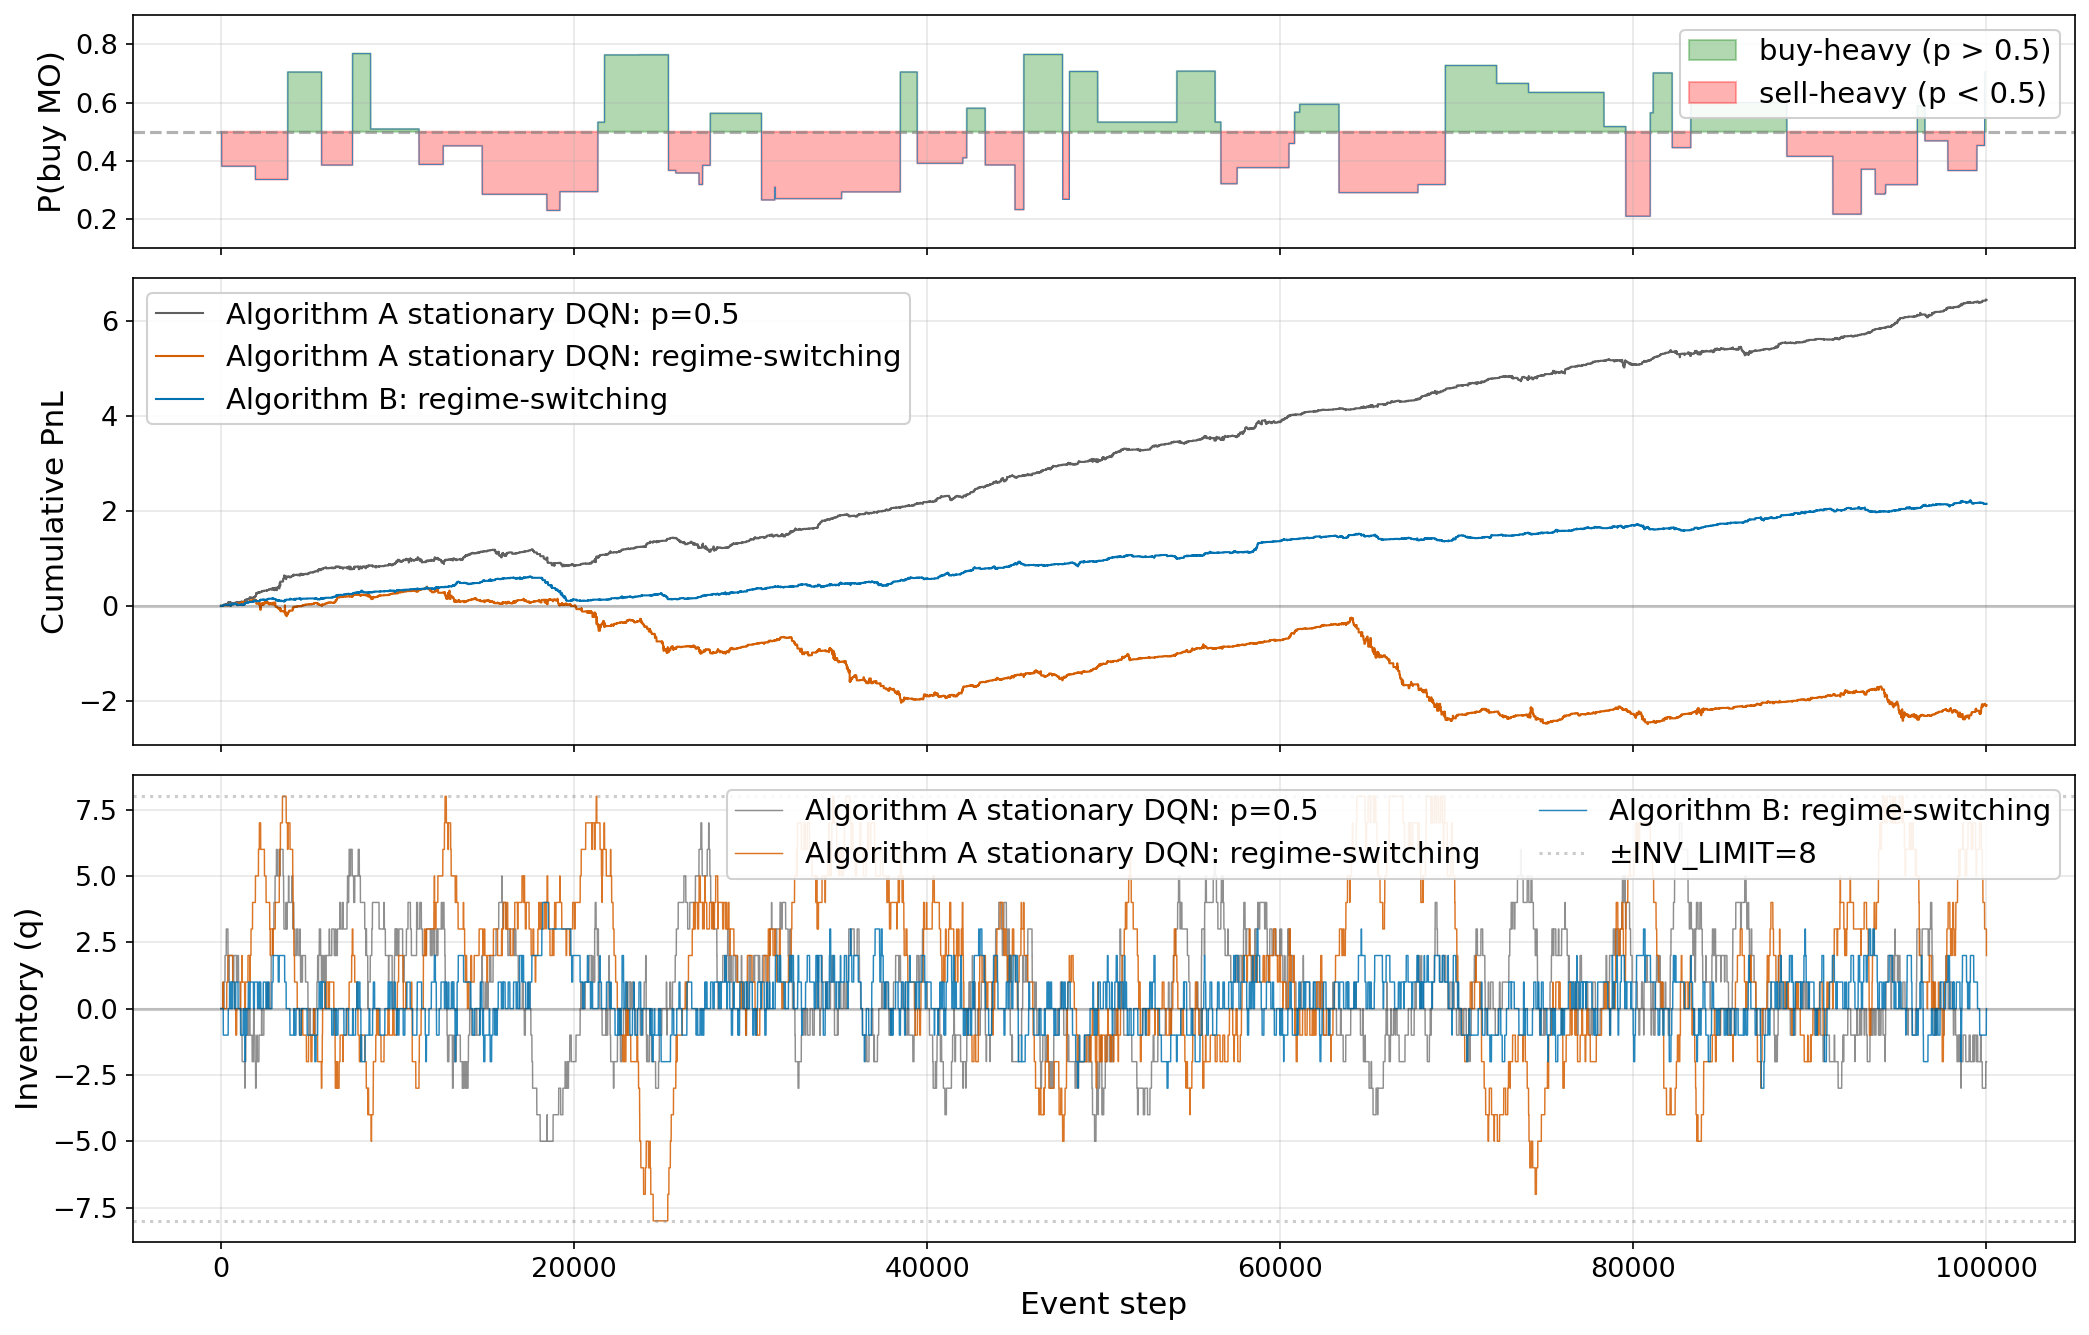
\includegraphics[width=0.8\linewidth]{regime_trained_final_phase_b.png}
  \caption{Algorithm~B evaluation under regime-switching flow
  ($\tau_r = 60$ MO events, $\omega = 0.30$).  Top: latent
  $p_{\mathrm{buy}}$ schedule (green = buy-heavy, red = sell-heavy).
  Middle: cumulative PnL for Algorithm~A at symmetric flow (gray), Algorithm~A
  under regime-switching (orange), and Algorithm~B (blue).  Bottom:
  inventory; Algorithm~B (blue) stays in a tight band while the
  non-adapted Algorithm~A (orange) repeatedly saturates at the
  $\pm q_{\max}$ caps.}
  \label{fig:regime_trained}
\end{figure}

\paragraph{Monte-Carlo simulations.}
To verify that the single-episode picture above is not a favorable
realization, we run $N_{\mathrm{sim}} = 100$ paired-seed episodes
of $N_{\mathrm{steps}} = 100\,000$ LOB events at $\tau_r = 60$ MO
events, $\omega = 0.30$.  Figure~\ref{fig:regime_trained_mean}
reports the mean cumulative PnL $\pm 1$~std across episodes for the
three policies.  Normalizing by the mean terminal PnL of the
Algorithm~A symmetric-flow benchmark, the non-adapted Algorithm~A controller under
regime-switching falls to roughly $-46\%$, while the Algorithm~B controller
ends around $37\%$.  The paired recovery of Algorithm~B relative to the
non-adapted Algorithm~A controller is therefore about $80\%$ of the
stationary Algorithm~A benchmark.  A paired $t$-test on terminal PnL rejects
equality at the $0.01\%$ level ($p < 10^{-4}$), so the
improvement is not only economically large but also statistically
unambiguous.

\begin{figure}[htbp]
  \centering
  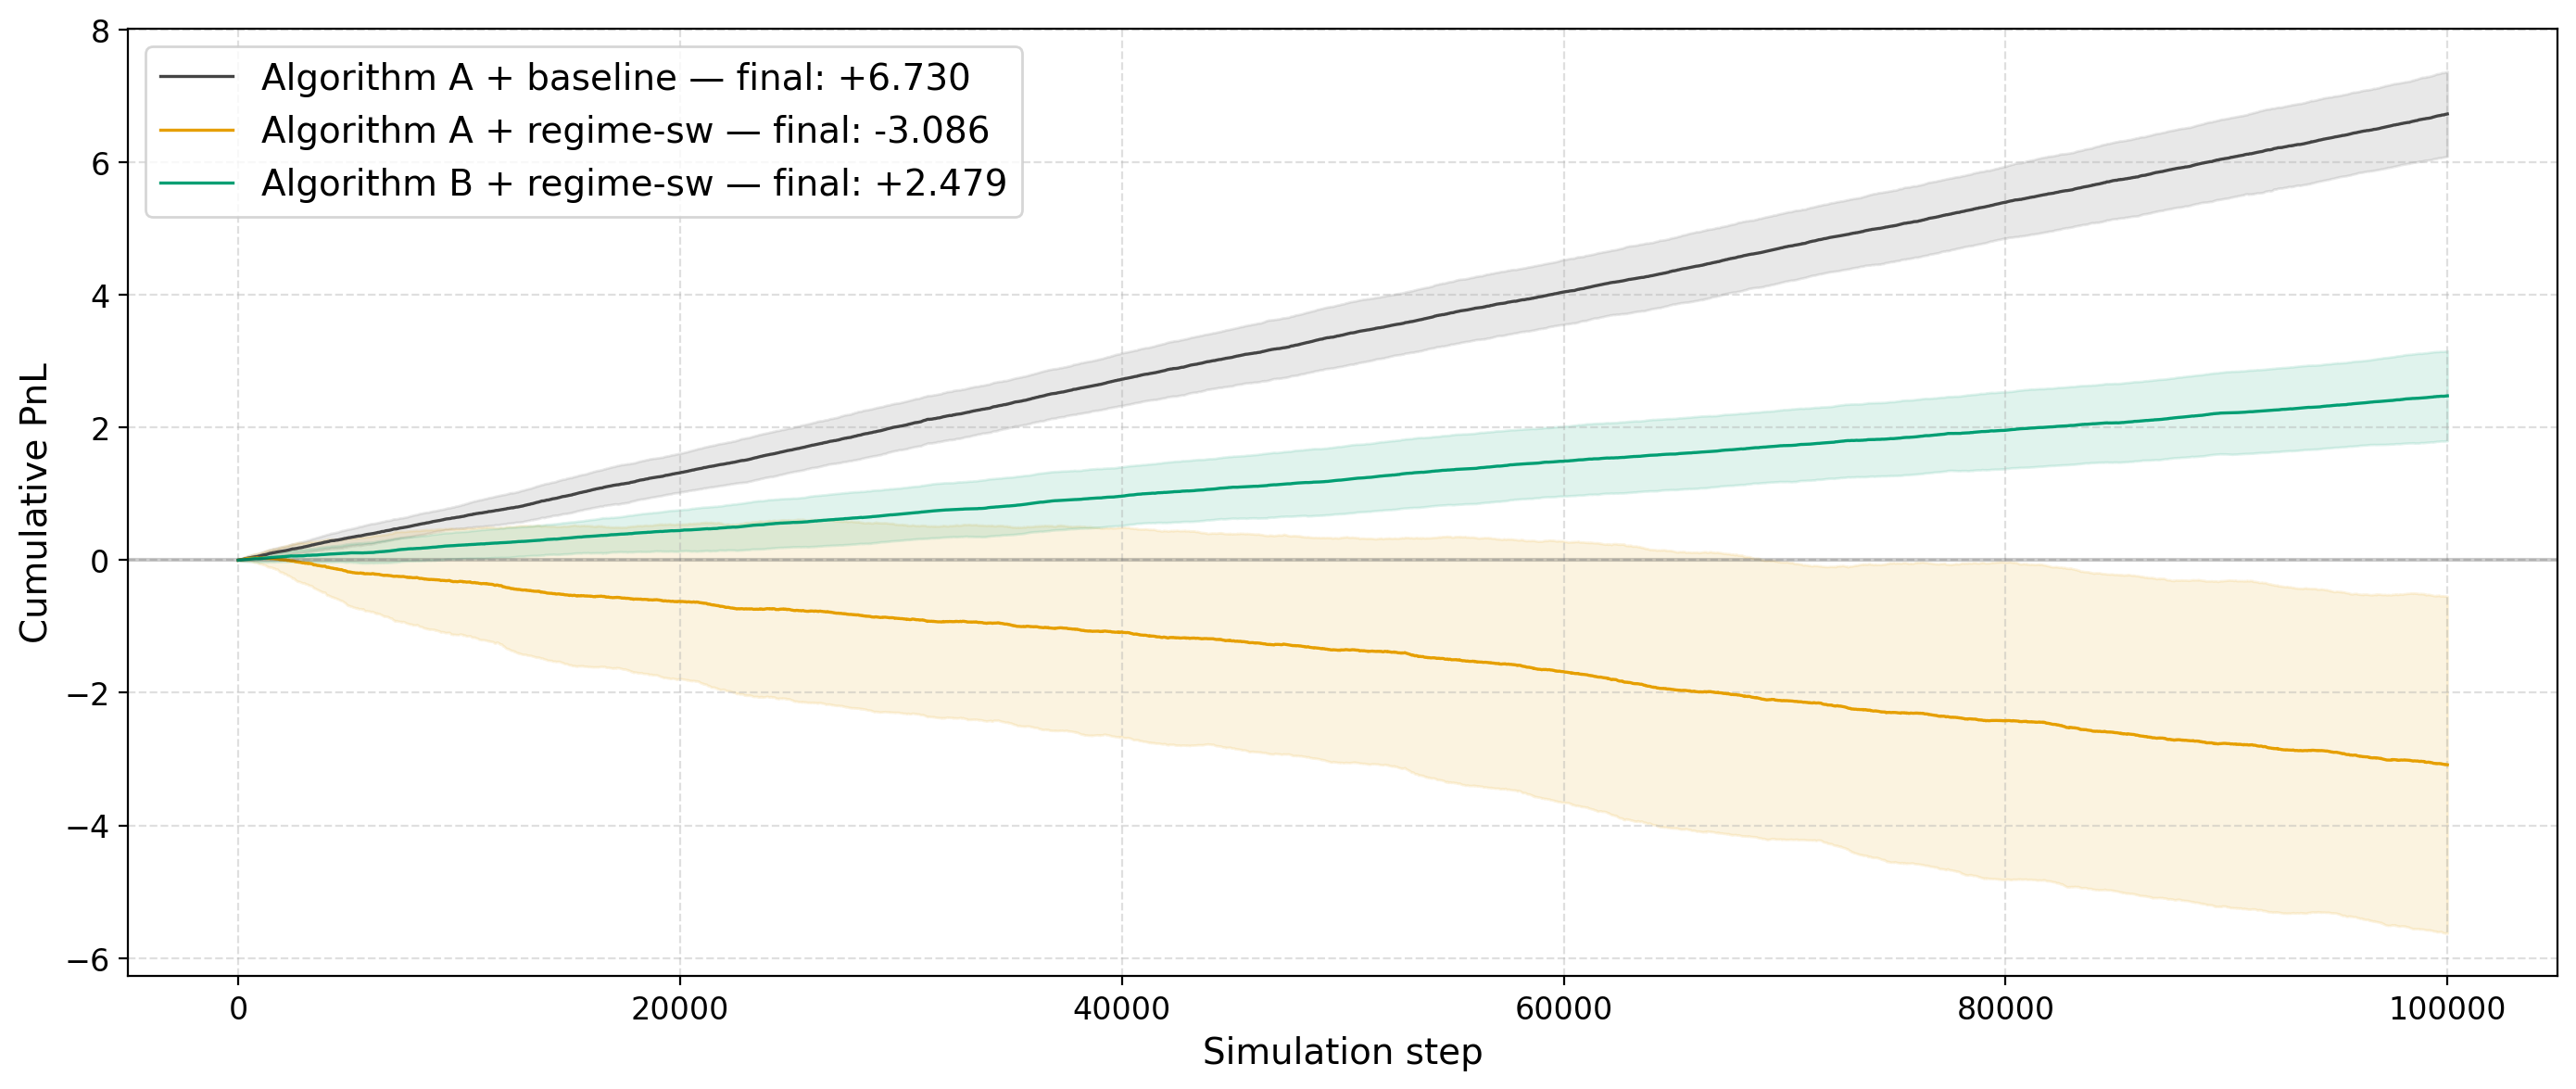
\includegraphics[width=0.7\linewidth]{regime_trained_pnl_mean_across_time.png}
  \caption{Monte-Carlo cumulative PnL (mean $\pm 1$ std) over
  $N_{\mathrm{sim}} = 100$ paired-seed episodes of
  $N_{\mathrm{steps}} = 100\,000$ LOB events ($\tau_r = 60$,
  $p_{\mathrm{buy}} \in [0.20, 0.80]$): Algorithm~A at symmetric flow
  (gray), Algorithm~A under regime-switching (orange), and Algorithm~B (green).
  Algorithm~B returns to a profitable regime; magnitudes in the text.}
  \label{fig:regime_trained_mean}
\end{figure}

\paragraph{Inventory control.}
Figure~\ref{fig:regime_trained_inv} aggregates the inventory
trajectories from the same Monte-Carlo run.  The time-averaged
inventory standard deviation is normalized to the Algorithm~A
symmetric-flow baseline.  Under regime-switching, the non-adapted
Algorithm~A controller widens to $1.89\times$ that baseline, as directional
regimes drag the position to the caps, whereas Algorithm~B contracts to
$0.55\times$ the same baseline.  Algorithm~B more than closes the
regime-induced inventory dispersion gap, confirming that the PnL gain
comes from genuine inventory containment rather than from lucky
directional bets.

\begin{figure}[htbp]
  \centering
  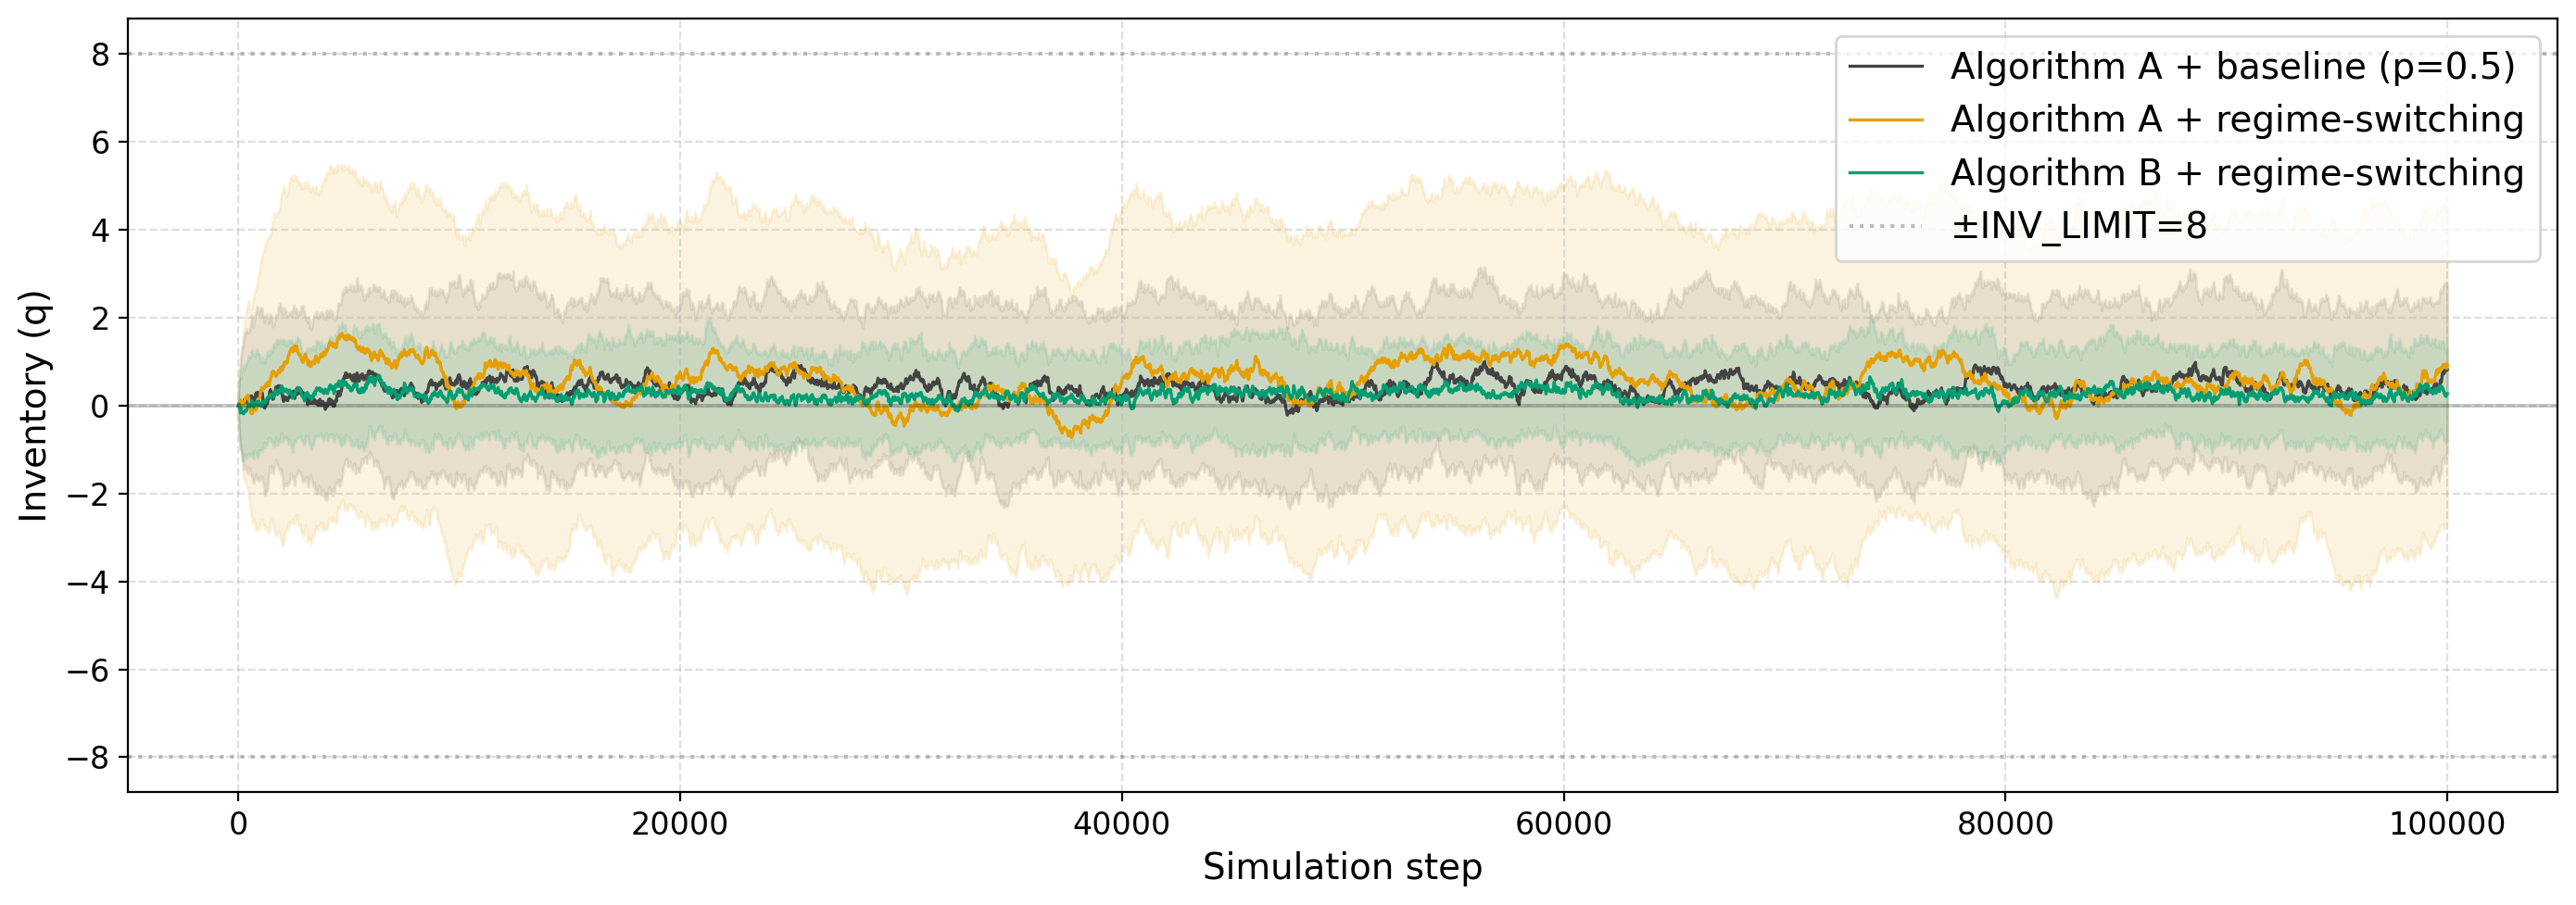
\includegraphics[width=0.7\linewidth]{inventory_distribution_phaseA_phaseB.png}
  \caption{Monte-Carlo inventory trajectory (mean $\pm 1$ std) over the
  same $N_{\mathrm{sim}} = 100$ episodes: Algorithm~A at symmetric flow
  (gray), Algorithm~A under regime-switching (orange), and Algorithm~B (green).
  Dashed lines mark the $\pm q_{\max} = 8$ cap; dispersion ratios in the
  text.}
  \label{fig:regime_trained_inv}
\end{figure}

\paragraph{Terminal-PnL distributions.}
Figure~\ref{fig:pnl_distribution} plots the histograms of
the raw terminal PnL in the same $N_{\mathrm{sim}} = 100$ episodes. The Algorithm~A baseline (gray) is
tightly concentrated, reflecting controlled spread capture under
symmetric flow.  Under regime-switching, the non-adapted Algorithm~A
distribution widens sharply and shifts to negative raw PnL.  The
Algorithm~B distribution (green), on the contrary, shifts back into positive
raw PnL and is substantially tighter than the regime-switching
distribution of the non-adapted Algorithm~A controller (its width is comparable
to the symmetric-flow baseline: $10\%$ vs.\ $10\%$); its mean
corresponds to a little over one third of the stationary Algorithm~A benchmark
rather than a loss-making outcome.

\begin{figure}[htbp]
  \centering
  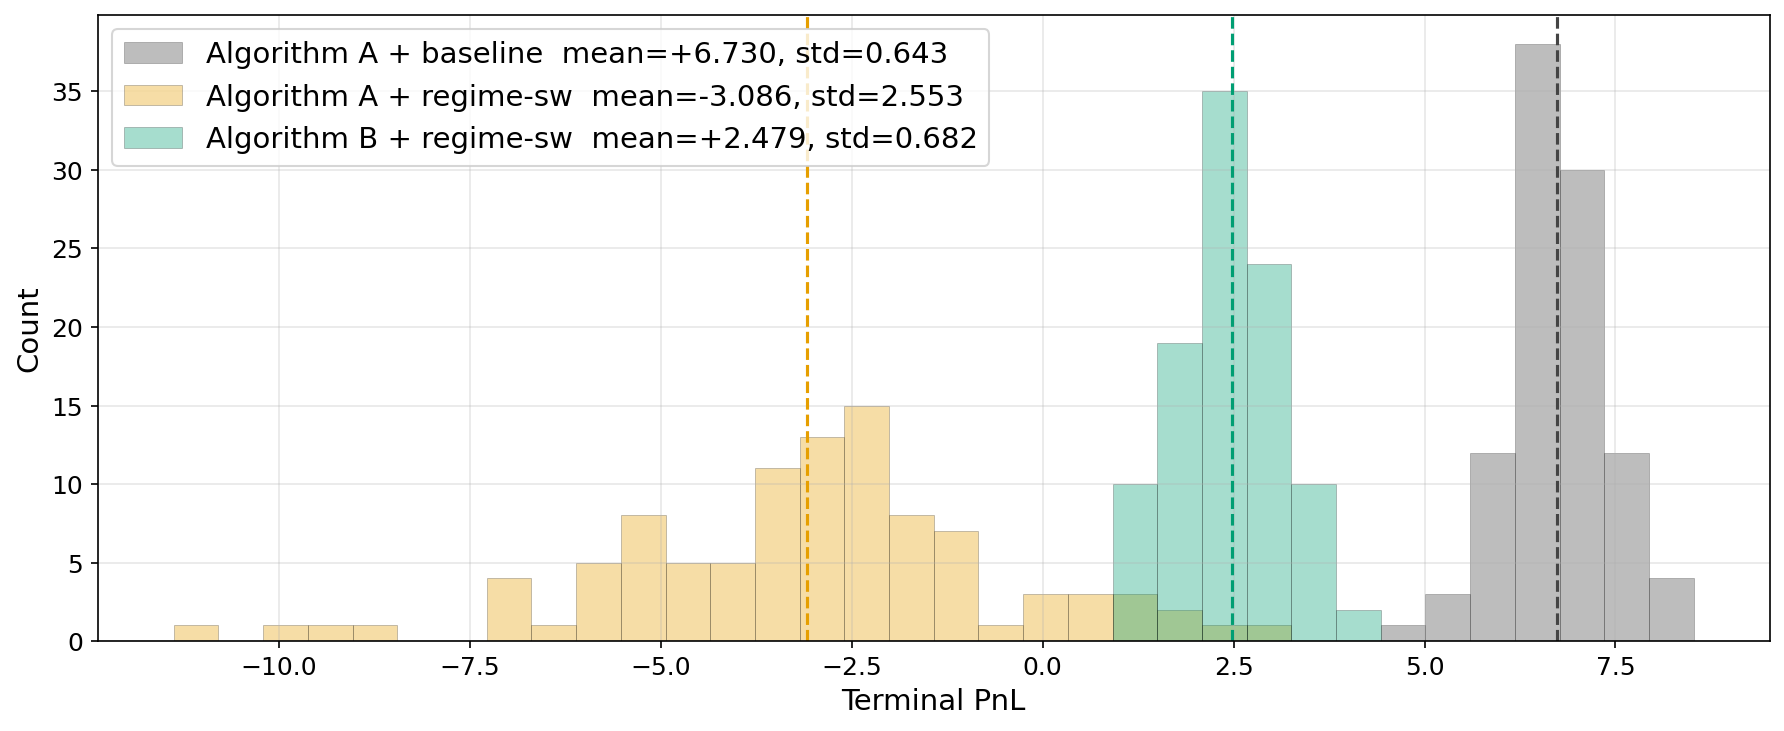
\includegraphics[width=0.7\linewidth]{pnl_distribution_phaseA_phaseB.png}
  \caption{Terminal-PnL histograms across $N_{\mathrm{sim}} = 100$
  paired-seed episodes ($N_{\mathrm{steps}} = 100\,000$ events).
  Relative to the Algorithm~A symmetric-flow mean, the (mean, std) are
  $(100\%,10\%)$ for Algorithm~A symmetric flow (gray), $(-46\%,38\%)$ for
  Algorithm~A under regime-switching (orange), and $(37\%,10\%)$ for
  Algorithm~B (green); dashed lines mark the per-policy means.  The
  Algorithm~B distribution is shifted right and substantially tighter than
  the non-adapted regime-switching distribution, indicating a
  robustness gain rather than a lucky tail.}
  \label{fig:pnl_distribution}
\end{figure}

\section{Interpreting the Regime-Trained Policy}
\label{sec:interpretability}

The goal of this section is to verify that the Algorithm~B controller is
not merely a black box that scores well on PnL, but a policy whose
learned value function reflects the economic intuition that motivated
its state design.  Concretely, we ask whether the network uses the
inferred regime, the inventory, the available spread, and the
quote-exposure signal in the directions predicted by the classical market-making
theory.

The Algorithm~B controller is not a closed-form quoting rule, but its
learned value function can still be interrogated locally.  We do this
by anchoring each probe at a representative state observed at a
controller decision epoch in a regime-switching evaluation episode.
Holding all remaining state coordinates fixed at their observed
values, we vary two economically meaningful features on a grid.  At
each point on the grid, we evaluate the C51 network through its implied scalar
value.
\begin{equation}
  \widehat V_\theta(s)
  =
  \max_{a\in\mathcal A} Q_\theta(s,a)
  =
  \max_{a\in\mathcal A}
  \sum_{i=1}^{N} z_i\,\pi_i(s,a),
\end{equation}
where maximization is over the six quoting actions used by the
agent, and the second equality uses the C51 representation of each
action value as the mean of its categorical return distribution; the
atom support $\{z_i\}_{i=1}^{N}$ and the atom count $N=101$ are those
 introduced for the C51 head in Section~\ref{sec:learning_formulation}.
These plots are therefore local sensitivity slices of the learned
value surface.

\paragraph{Heatmap slices.}
Figure~\ref{fig:interp_heatmaps} reports three heatmap slices of the
Algorithm~B learned value function $\widehat V_\theta(s)=\max_a Q_\theta(s,a)$,
each varying the two state coordinates shown on its axes.  In
Figure~\ref{fig:interp_heatmaps}(\subref{fig:interp_heat_inv_bayes}),
the inventory--regime slice shows the clearest inventory-skew logic:
value is largest near zero inventory and falls sharply close to the
hard caps.  Conditional on a non-zero inventory, the Bayesian belief
shifts the value surface in the direction predicted by market-making
economics.  A long inventory is less dangerous when the filter detects
buy-heavy flow, because ask fills are more likely and tend to reduce
the position; a short inventory is less dangerous under sell-heavy flow
for the symmetric reason. The inventory spread slice in
Figure~\ref{fig:interp_heatmaps}(\subref{fig:interp_heat_inv_spread})
separates the spread opportunity from the inventory risk: wider spreads
increase the value near the center of the inventory band, but do not
rescue states near $|q|=q_{\max}$.  The regime--spread slice in
Figure~\ref{fig:interp_heatmaps}(\subref{fig:interp_heat_bayes_spread})
shows the complementary effect: large spreads are valuable, but the
value gain is attenuated when the inferred directional regime is
extreme.  Together, these local slices are consistent with Algorithm~B
having internalized the qualitative trade-off that motivated its reward
design---capture spread only when doing so does not push inventory into
a one-sided regime---although they probe the value surface only around
representative anchor states.

\begin{figure}[htbp]
  \centering
  % Three heatmaps side by side (widened into margins for legibility).
  \makebox[\linewidth][c]{%
  \begin{minipage}{1.18\linewidth}
  \centering
  \begin{subfigure}[t]{0.333\linewidth}
    \centering
    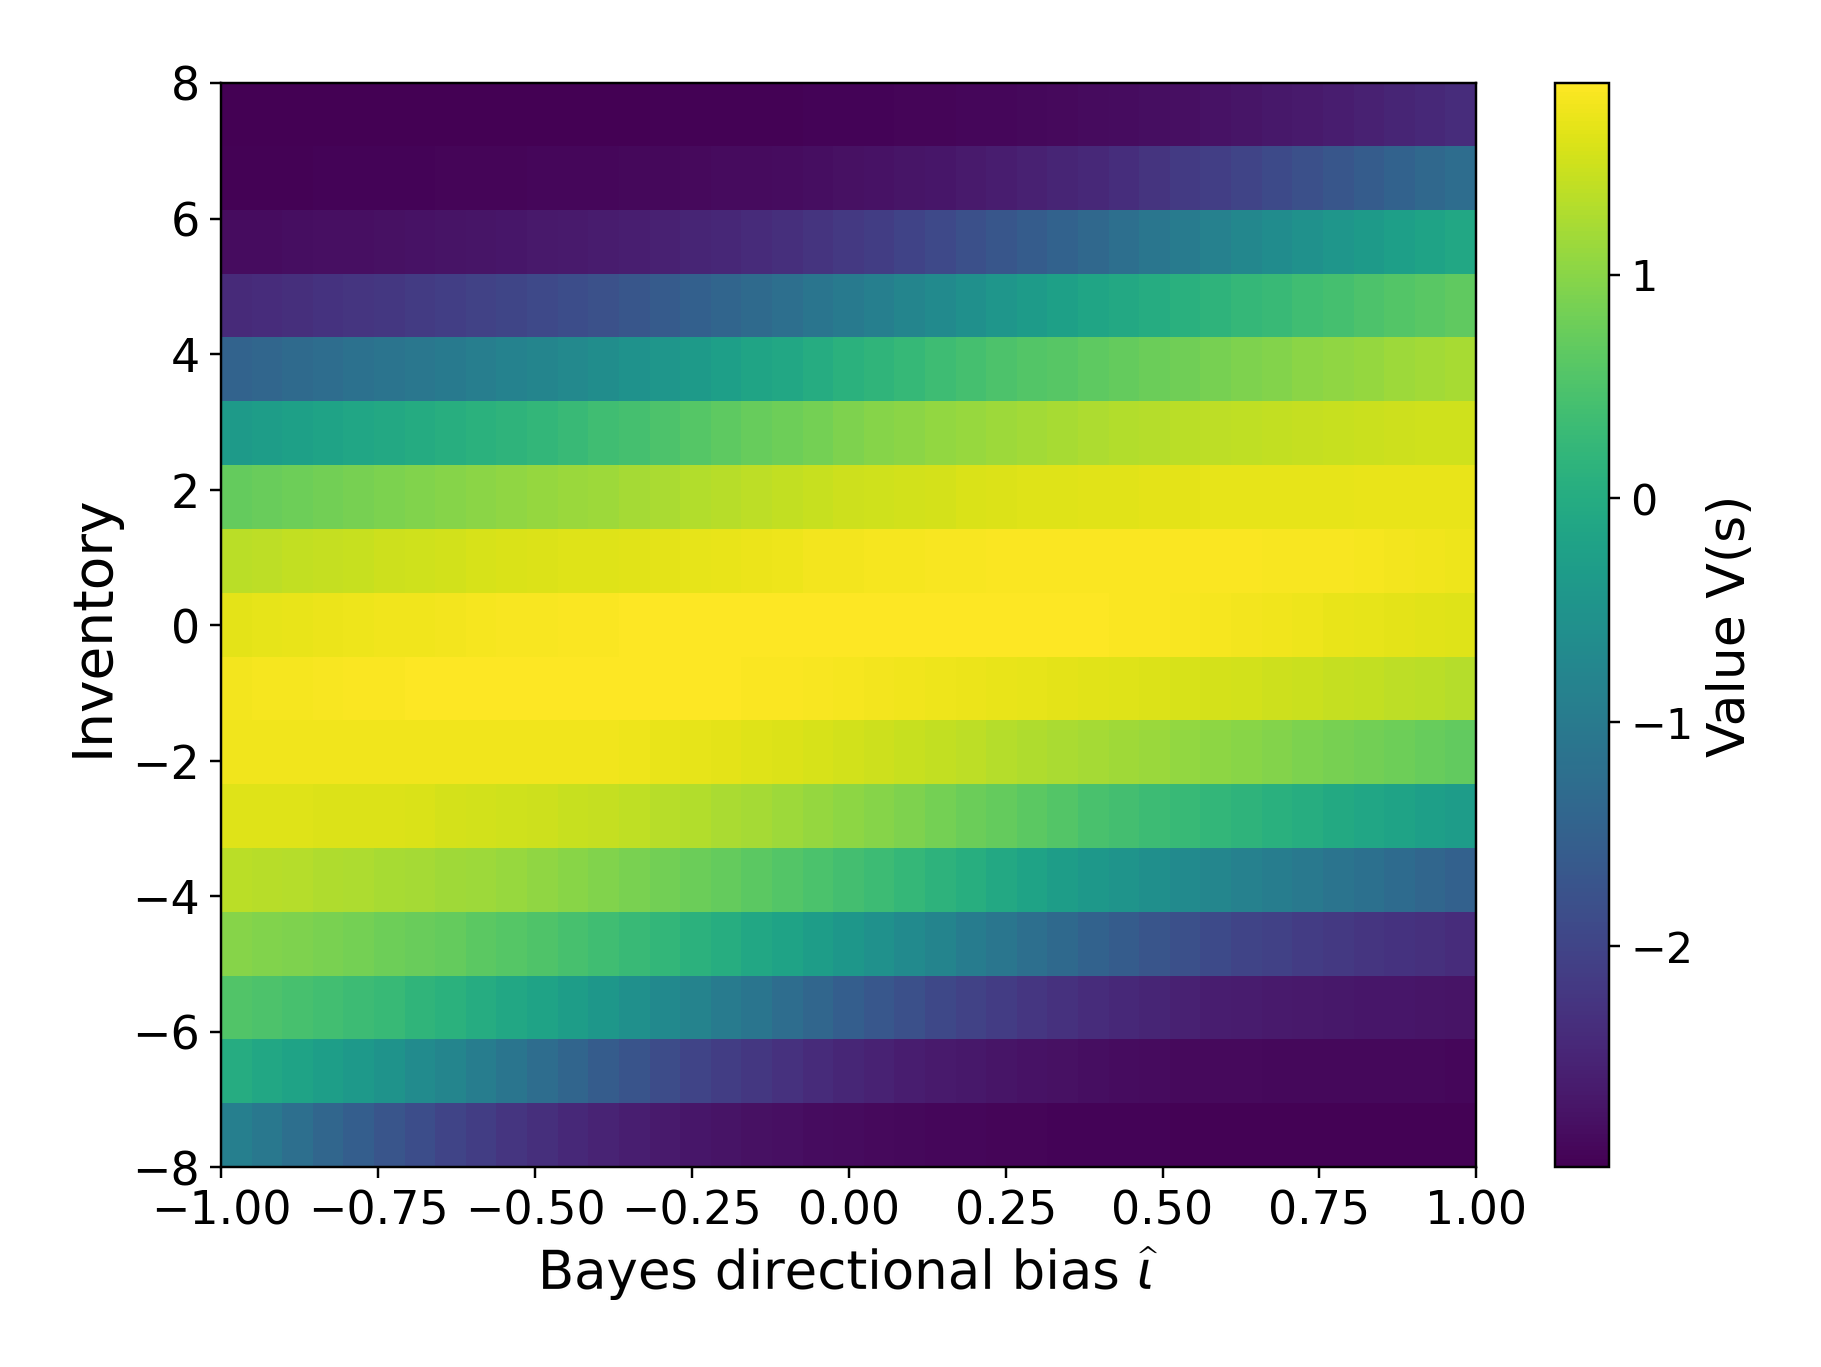
\includegraphics[width=\linewidth]{p_buy_mhat_vs_inv.png}
    \caption{Inventory and Bayesian bias.}
    \label{fig:interp_heat_inv_bayes}
  \end{subfigure}\hfill
  \begin{subfigure}[t]{0.333\linewidth}
    \centering
    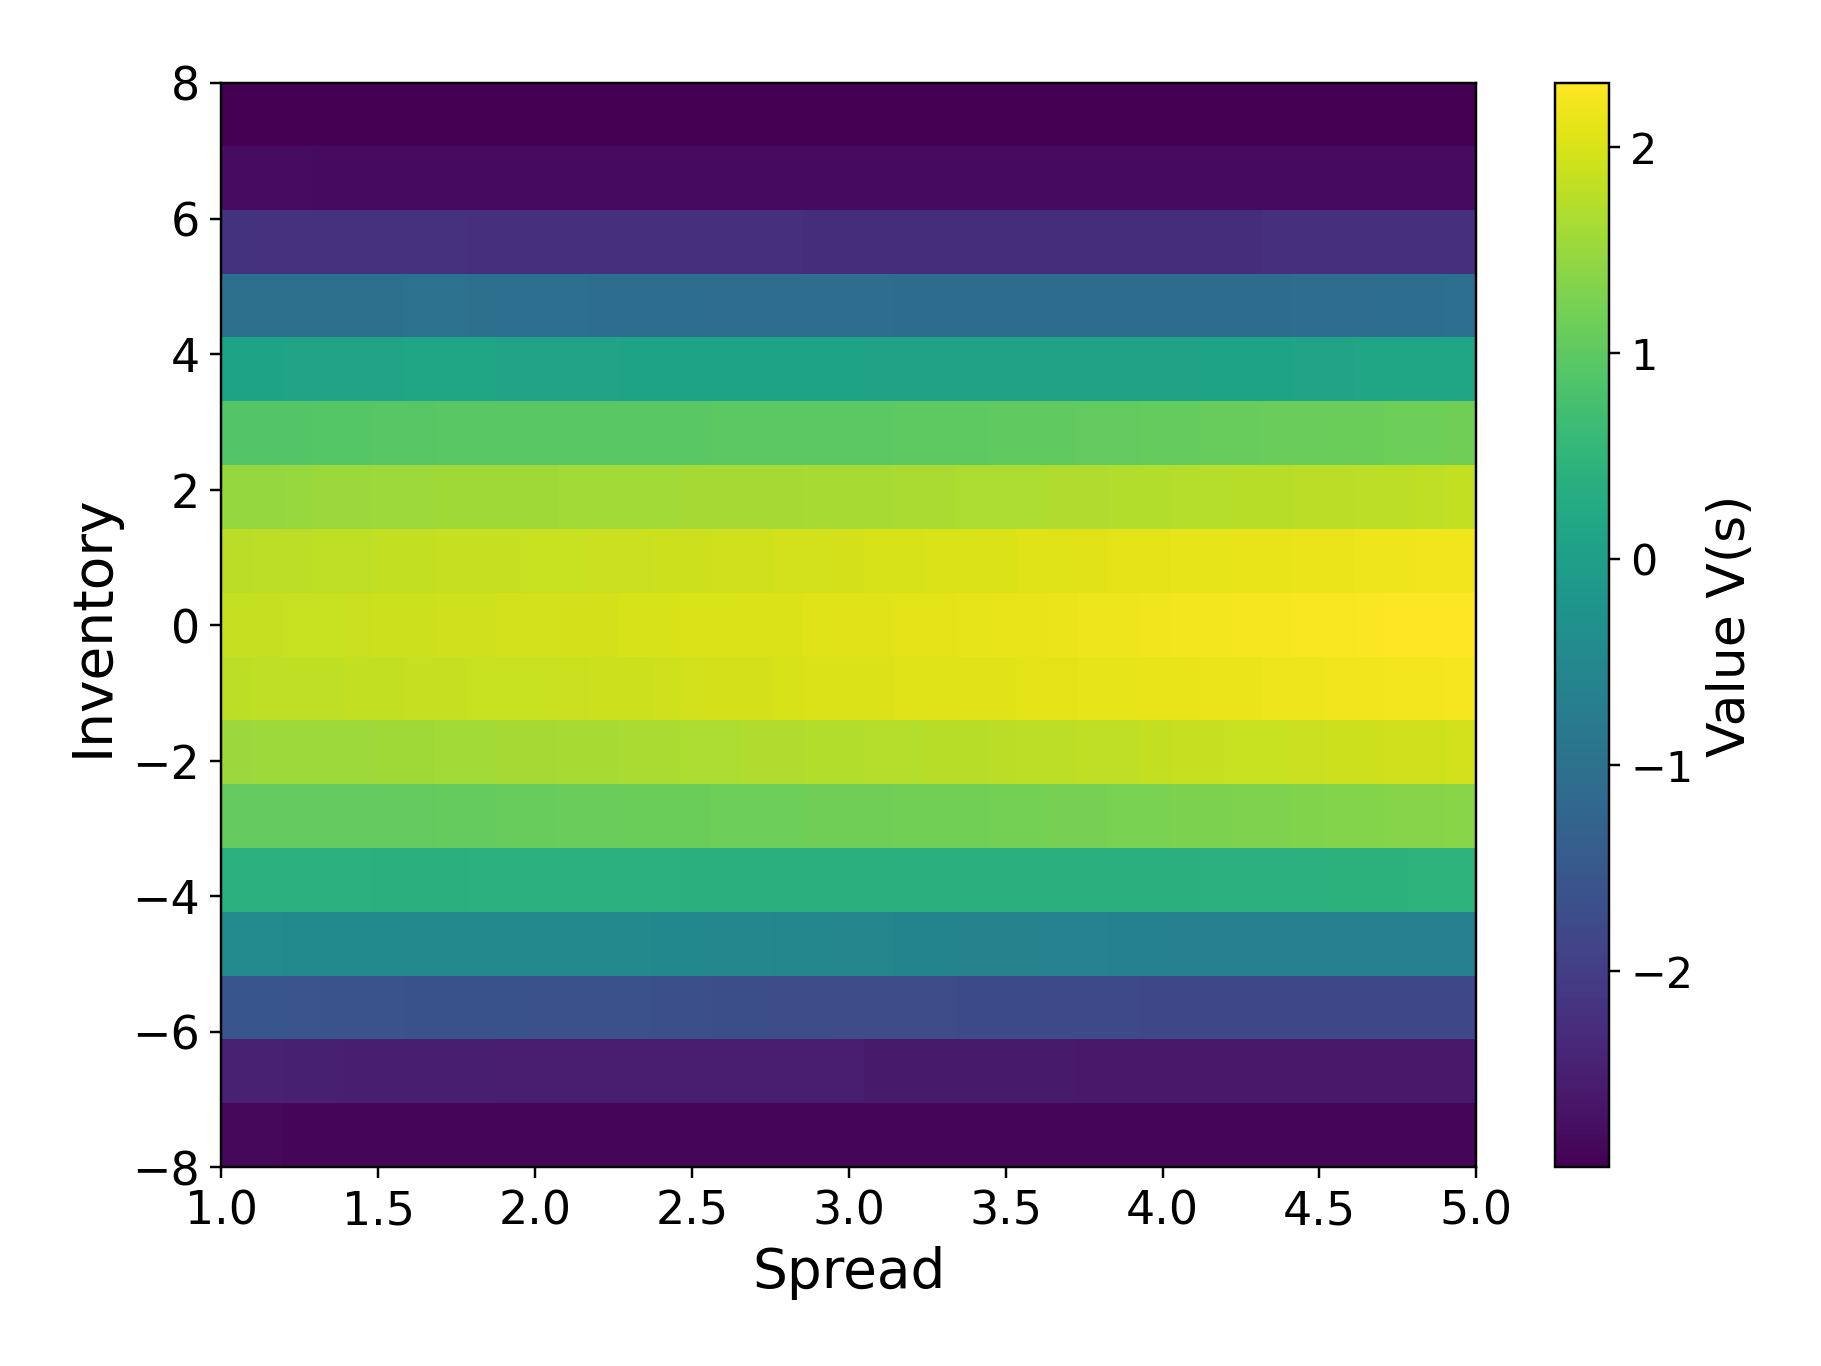
\includegraphics[width=\linewidth]{inventory_vs_spread.png}
    \caption{Inventory and spread.}
    \label{fig:interp_heat_inv_spread}
  \end{subfigure}\hfill
  \begin{subfigure}[t]{0.333\linewidth}
    \centering
    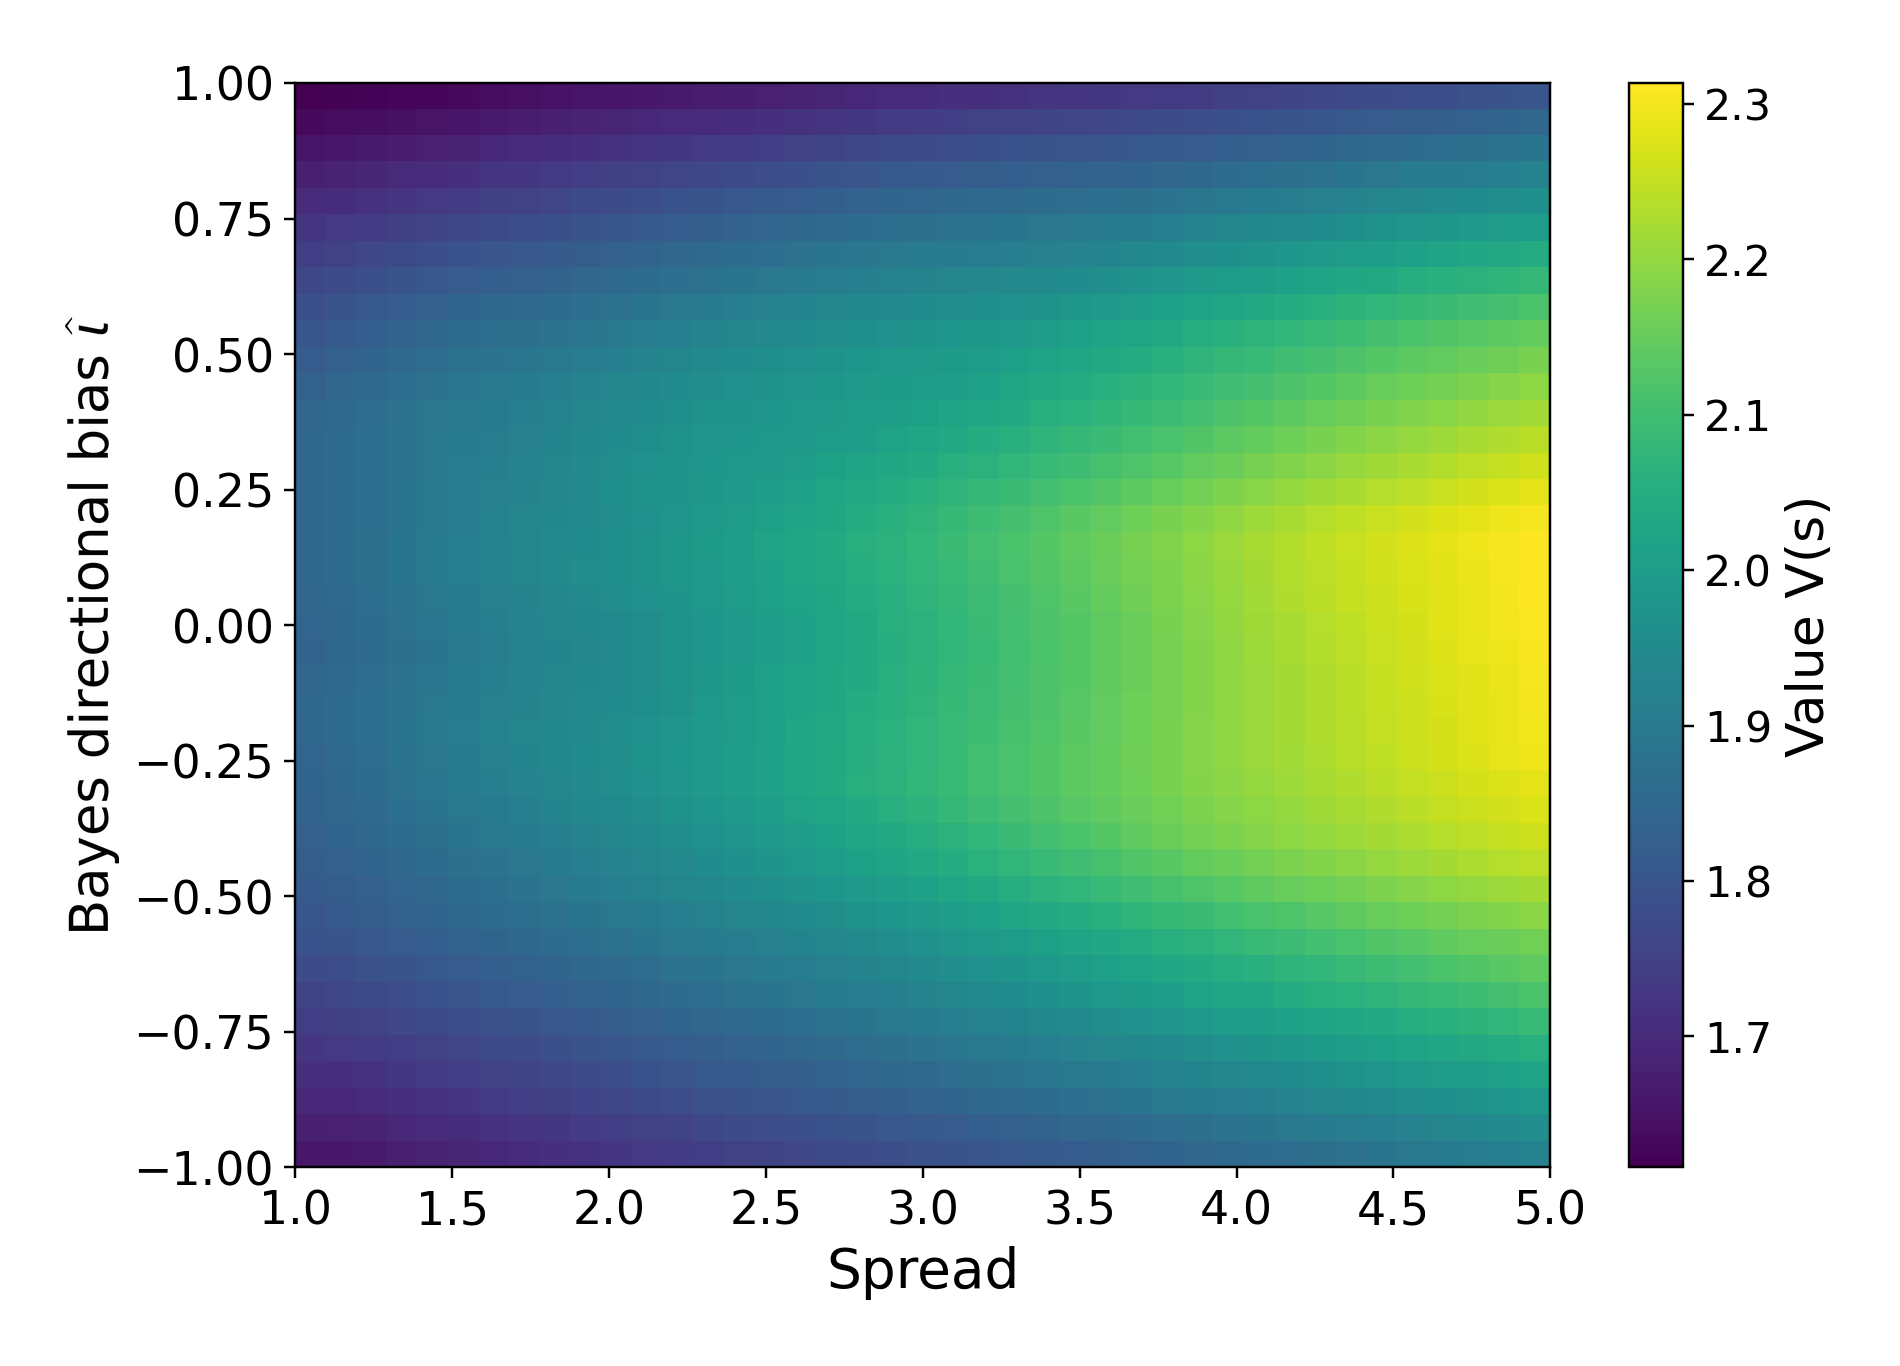
\includegraphics[width=\linewidth]{bayes_m_vs_spread.png}
    \caption{Bayesian bias and spread.}
    \label{fig:interp_heat_bayes_spread}
  \end{subfigure}
  \end{minipage}}
  \caption{Heatmap slices of the Algorithm~B value function: value as a
  function of (a)~inventory and Bayesian directional bias, (b)~inventory
  and spread, and (c)~Bayesian directional bias and spread.}
  \label{fig:interp_heatmaps}
\end{figure}


\paragraph{Auxiliary-signal diagnostics.}
Finally, Figure~\ref{fig:interp_signal_examples} shows the signals
sent to the regime-trained controller during representative episodes.
The Bayesian filter tracks the latent directional bias
$2p_{\mathrm{buy}}(t)-1$ without observing the simulator's regime
labels.  Its posterior mean $\widehat{\iota}_t$ follows the true regime
while smoothing individual market-order noise; the expected run length
increases within a regime before dropping at detected changes.  The
quote-exposure diagnostic shows the complementary endogenous signal
$x_t$ of Eq.~\eqref{eq:quote_exposure_imbalance}: it reacts
immediately to the agent's own live queue position and so summarizes,
along the episode, the fill asymmetry created by the current resting
quotes (range $[-1/2,1/2]$ under unit quotes).  The feature is thus
forward-looking, telling the policy which side of the book is more
vulnerable before the next market order arrives.

\begin{figure}[htbp]
  \centering
  \begin{subfigure}[b]{0.7\linewidth}
    \centering
    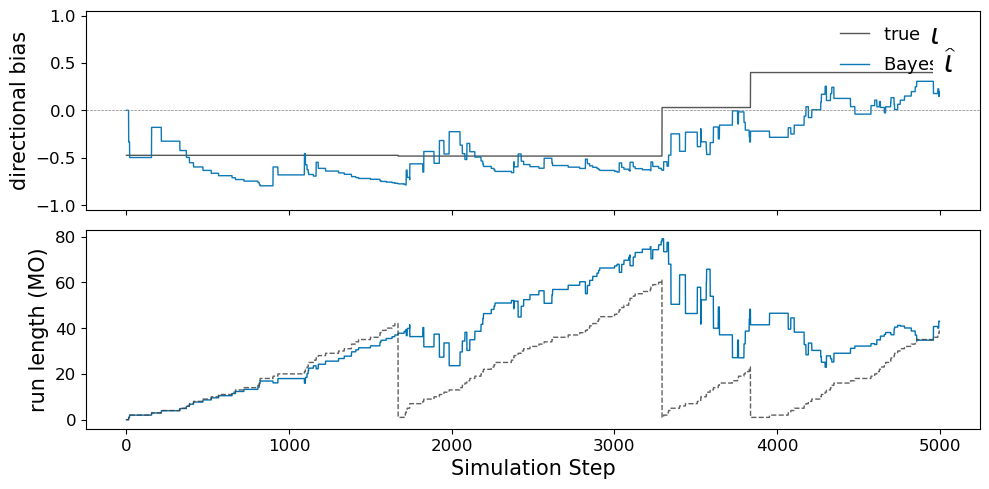
\includegraphics[width=\linewidth]{bayes_single_estimation_example.png}
    \caption{Bayesian regime-belief diagnostics.}
    \label{fig:interp_bayes_example}
  \end{subfigure}

  \vspace{6pt}

  \begin{subfigure}[b]{0.7\linewidth}
    \centering
    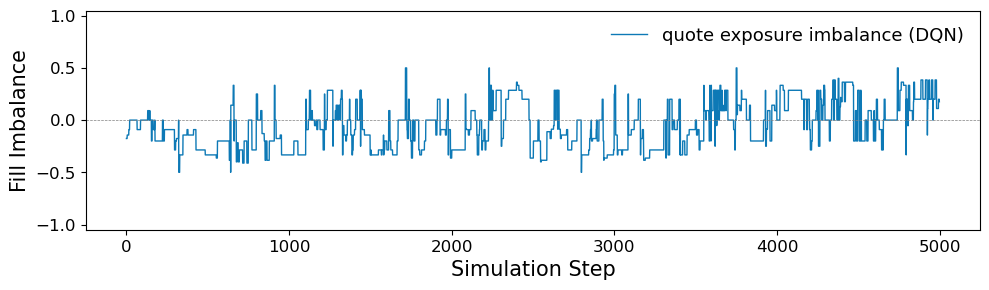
\includegraphics[width=\linewidth]{quote_exposure_single_estimation_example.png}
    \caption{Quote-exposure imbalance diagnostic.}
    \label{fig:interp_quote_exposure_example}
  \end{subfigure}
  \caption{Representative-episode diagnostics for the auxiliary signals used
  by Algorithm~B (each panel shows one representative evaluation episode).
  The Bayesian filter provides a smoothed belief over the
  latent directional regime and its run length, while the
  queue-adjusted quote-exposure imbalance provides an instantaneous
  measure of the asymmetry in the agent's own resting quotes.}
  \label{fig:interp_signal_examples}
\end{figure}

\section{Out-of-Distribution Regime Stress Tests}
\label{sec:stress_tests}

The Algorithm~B evaluation above matches the training family
($\tau_r = 60$ MO events, $p_{\mathrm{buy}} \in [0.20, 0.80]$).  To test
whether the controller learned a genuinely robust response rather than a
policy tuned to that single persistence scale, we run three paired-seed
stress diagnostics: within each panel the compared policies or
specifications share the same exogenous seed and differ only in the
regime-generation rule.  The last two use longer episodes
($500\,000$ vs.\ $100\,000$ LOB events), so their PnL levels should be
read within each figure.

\paragraph{Persistence sweep.}
We sweep the mean regime duration $\tau_r \in \{15,30,60,120,240\}$ MO
events at fixed width $p_{\mathrm{buy}}\in[0.20, 0.80]$, evaluating both
the stationary Algorithm~A and the Algorithm~B controller over $N_{\mathrm{sim}}=100$
paired episodes of $100\,000$ LOB events~(Figure~\ref{fig:phaseb_tau_sweep});
the Algorithm~A curve reproduces the degradation of
Figure~\ref{fig:degradation_tau} and is shown again only as the
reference against Algorithm~B.  Algorithm~A decays monotonically, from about
$30\%$ at $\tau_r=15$ to $-91\%$ at $\tau_r=240$, loss-making once
regimes are persistent.  Algorithm~B stays
profitable throughout, falling only from about $46\%$ to $23\%$: it
gives up part of the stationary spread-capture edge but does not
collapse under long-lived directional pressure.

\begin{figure}[htbp]
  \centering
  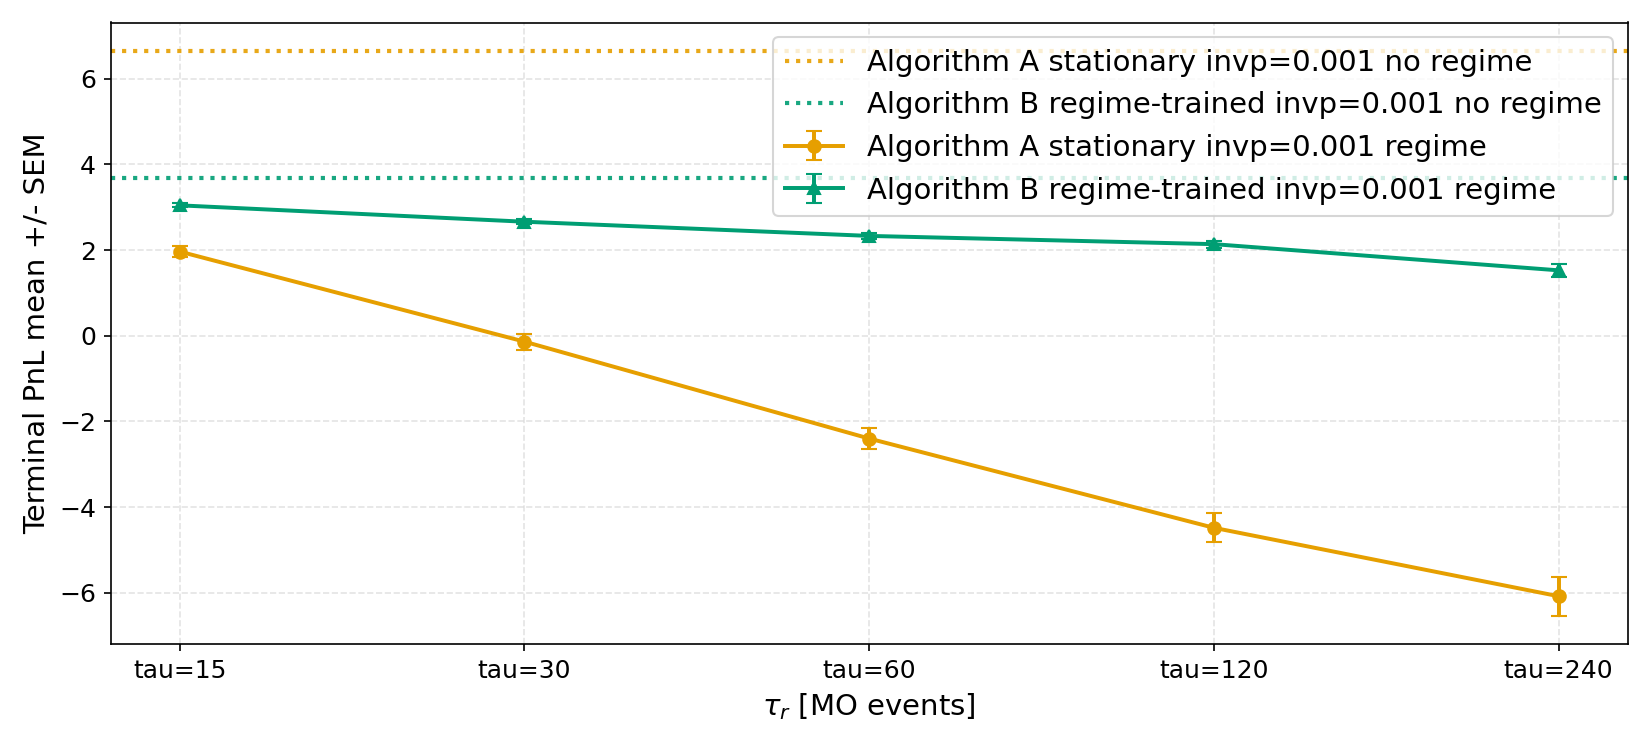
\includegraphics[width=0.7\linewidth]{regime_tau_sweep_decay_phasea_vs_phaseb.png}
  \caption{Persistence stress test over
  $\tau_r\in\{15,30,60,120,240\}$ MO events at fixed
  $p_{\mathrm{buy}}\in[0.20, 0.80]$ ($N_{\mathrm{sim}} = 100$ paired
  episodes of $N_{\mathrm{steps}} = 100\,000$ events,
  $\varphi = 10^{-3}$).  Mean terminal PnL $\pm$ SEM per $\tau_r$ value
  for the Algorithm~A and Algorithm~B controllers, each with its no-regime reference
  (horizontal line).  Algorithm~A decays monotonically and becomes
  loss-making at large $\tau_r$, whereas Algorithm~B stays profitable at
  every scale.}
  \label{fig:phaseb_tau_sweep}
\end{figure}

\paragraph{Random persistence within an episode.}
Here, each regime draws its own scale
$\tau_k\sim\mathrm{Uniform}\{15,30,60,120,240\}$, then length
$L_k\sim\mathrm{Exp}(1/\tau_k)$ and $p_{\mathrm{buy}}\in[0.20,0.80]$; the
agent does not observe $\tau_k$.  Against the fixed-$\tau_r=60$ benchmark
over $N_{\mathrm{sim}}=50$ paired episodes of $500\,000$ events
(Figure~\ref{fig:random_tau_stress}), the mean terminal PnL drops only about
$6.9\%$.  The effect is distributional rather than central: random
persistence widens the paired-effect distribution and thickens its left
tail. Thus, Algorithm~B remains robust to randomizing the memory scale, at the
cost of higher tail risk.

\begin{figure}[htbp]
  \centering
  \begin{subfigure}[t]{0.48\textwidth}
    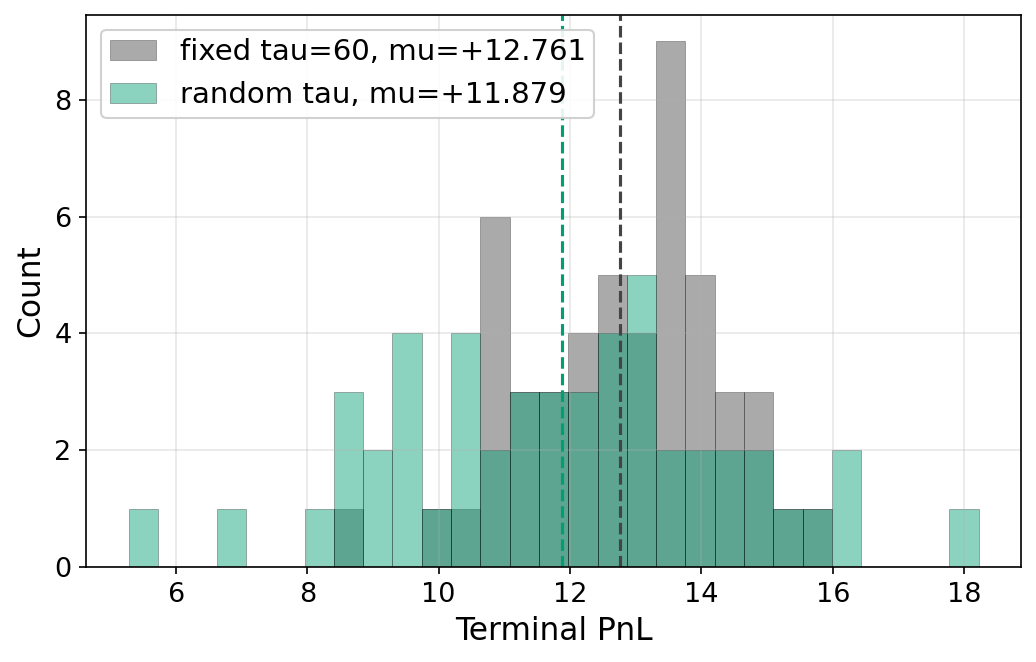
\includegraphics[width=\linewidth]{random_tau_stress.png}
    \caption{Random-persistence stress: each regime draws its own
    $\tau_k\in\{15,30,60,120,240\}$ before its exponential duration,
    vs.\ a fixed-$\tau_r=60$ benchmark.  The main change is increased
    left-tail risk.}
    \label{fig:random_tau_stress}
  \end{subfigure}
  \hfill
  \begin{subfigure}[t]{0.48\textwidth}
    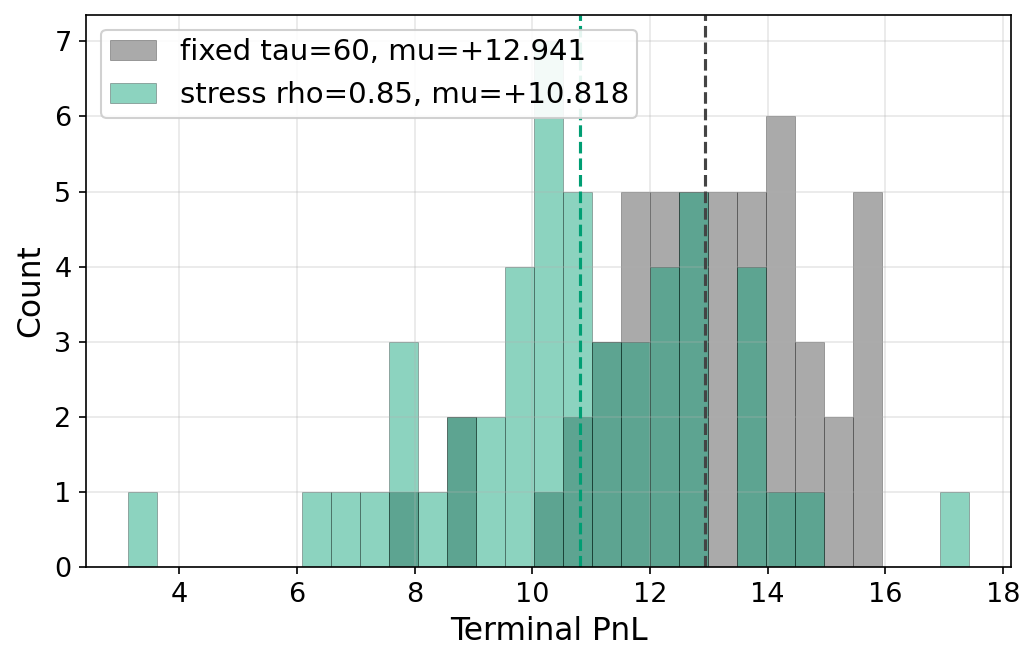
\includegraphics[width=\linewidth]{correlated_regime_stress.png}
    \caption{Correlated-direction stress: same per-regime random-$\tau_k$
    duration mechanism as the previous panel
    ($\tau_k\sim\mathrm{Uniform}\{15,30,60,120,240\}$), plus temporal
    correlation on the directional side: regime signs are retained with
    probability $\rho_{\mathrm{side}}=0.85$, imbalance intensity
    $I_k\sim\mathrm{Uniform}[0.00,0.30]$.
    The stress increases downside tail risk.}
    \label{fig:correlated_regime_stress}
  \end{subfigure}
  \caption{Algorithm~B stress tests, both over $N_{\mathrm{sim}}=50$
  paired episodes of $500\,000$ LOB events.  Terminal-PnL distributions
  vs.\ the fixed-$\tau_r=60$ benchmark.  Mean shifts in the text.}
  \label{fig:phaseB_stress_combined}
\end{figure}

\paragraph{Correlated directional regimes.}
Building on the random-persistence stress, we keep the same per-regime
random-$\tau_k$ duration mechanism ($\tau_k\sim\mathrm{Uniform}\{15,30,60,120,240\}$,
$L_k\sim\mathrm{Exp}(1/\tau_k)$) and add temporal correlation
on the directional side.  Concretely, at each regime boundary the
sign $s_k\in\{-1,+1\}$ is retained with probability
$\rho_{\mathrm{side}}=0.85$, the imbalance intensity (magnitude of the
deviation of $p_{\mathrm{buy},k}$ from the symmetric value $0.5$) is
$I_k\sim\mathrm{Uniform}[0.00,0.30]$, and
$p_{\mathrm{buy},k}=0.50+s_k I_k$.  This keeps the support
$p_{\mathrm{buy}}\in[0.20,0.80]$ but clusters the same-side pressure,
a harder adverse-selection environment.  Algorithm~B remains profitable
(Figure~\ref{fig:correlated_regime_stress}): the mean terminal PnL falls
about $16.4\%$ versus the fixed benchmark $\tau_r=60$, with a
substantially larger left tail, but without returning to the loss-making
regime of the stationarily trained controller.

Taken together, these tests support reading Algorithm~B as a robustness
intervention rather than a fit to a simulator seed or timescale: it
 continues to earn money when $\tau_r$ is swept far from the training point,
when persistence varies randomly between regimes, and when the regime
signs become highly correlated.  The remaining failure mode is not a
collapse of mean PnL but an increase in downside tail risk under the
most persistent, correlated paths.

\section{Algorithm C: Scenario-Bandit Robust Fine-Tuning}
\label{sec:scenario_bandit_finetuning}

The stress tests in Section~\ref{sec:stress_tests} are
evaluation-only: the Algorithm~B controller is trained on a single
regime-switching family (fixed $\tau_r=60$ MO events,
$p_{\mathrm{buy}}\in[0.20,0.80]$) and is then exposed to
random-persistence and correlated-direction shifts.  The remaining weakness is therefore a
lower-tail problem: the mean PnL remains positive, but some
realized regime scenarios still push the agent into unfavorable
inventory--flow alignment.  We address this with a scenario-bandit
robust fine-tuning step---our Algorithm~C.

A scenario $\xi$ is an exogenous regime plan rather than a full
reinforcement-learning trajectory.  It stores the sequence of regime
durations and buy-MO probabilities on the market-order clock,
together with the seed used to generate that sequence:
\[
  \xi_i
  =
  \bigl((\tau_{i,k},L_{i,k},p_{i,k})_{k=1}^{K_i},\,\zeta_i\bigr).
\]
Here $K_i$ denotes the (scenario-dependent) number of regimes stored in
$\xi_i$, chosen at generation time as the smallest count such that the
cumulative regime length $\sum_{k=1}^{K_i} L_{i,k}$ covers the expected
number of market orders $\widehat M$ in an episode
(Section~\ref{sec:nonstat_training}, Eq.~\eqref{eq:mo_horizon}).
The scalar $\zeta_i$ is the random seed used to generate the regime tuple;
the per-regime scale $\tau_{i,k}$ is retained only for reproducibility
and is not needed to evaluate the schedule.
The cumulative boundaries $C_{i,0}=0$ and
$C_{i,k}=\sum_{j=1}^k L_{i,j}$ define the continuous scalar schedule
$p_{\mathrm{buy}}^{\xi_i}(m)=p_{i,k}$ whenever
$C_{i,k-1}\le m<C_{i,k}$.  


The bandit acts over a finite pool of exogenous regime scenarios.
Each stored scenario is an arm: before a training episode, the
bandit selects one scenario, rolls out the current policy under that
scenario, observes the resulting terminal loss of that arm, and updates the arm's
difficulty score $d_i$---an exponential moving average of the
scenario's realized losses, defined in Eq.~\eqref{eq:difficulty_ewma}
below.  Scenarios that recently produced poor market-making performance
are sampled more often, redirecting the training effort toward the
empirical lower tail.


We now make the reference scenario generator $P_0$ precise.  Of the
three stress diagnostics of Section~\ref{sec:stress_tests}, the
persistence sweep is a grid of fixed evaluation settings rather than
a generative law; the other two are genuine generative families:
(i)~the \emph{random-persistence family}, which draws, independently
across regimes, $\tau_k\sim\mathrm{Uniform}\{15,30,60,120,240\}$,
$L_k\sim\mathrm{Exp}(1/\tau_k)$, and
$p_{\mathrm{buy},k}\sim\mathrm{Uniform}[0.20,0.80]$; and
(ii)~the \emph{correlated-direction family}, which uses the same
$(\tau_k,L_k)$ mechanism but sets
$p_{\mathrm{buy},k}=0.50+s_k I_k$, with the sign $s_k\in\{-1,+1\}$
retained across regime boundaries with probability
$\rho_{\mathrm{side}}=0.85$ and $I_k\sim\mathrm{Uniform}[0.00,0.30]$.
$P_0$ is the \emph{scenario-level} equal-weight mixture of these two
families: a draw $\xi\sim P_0$ first selects one of the two families
with a fair coin and then generates the entire regime schedule
$(\tau_k,L_k,p_k)_{k\ge1}$ from that family's law, appending regimes
until the cumulative length covers $\widehat M$ as described above.
The two families therefore mix only across scenarios, never within
one.  The pool
$\{\xi_i\}_{i=1}^{M}$, with $M=256$, is initialized with $128$
scenarios drawn from each family: a deterministic half-half split,
not an i.i.d.\ draw from $P_0$.  It is subsequently maintained by
the adaptive refresh mechanism described below, whose replacement
scenarios are i.i.d.\ draws from $P_0$.
Let $T$ denote the total number of MM decisions in an episode, so that
$t=0,1,\ldots,T-1$ indexes the decision grid of
Section~\ref{sec:learning_formulation}; ``terminal'' quantities below are
those evaluated once at $t=T$, after the last decision has been resolved.
Standard training resamples a new scenario each iteration from the
reference generator $P_0$ and updates the controller via the same
Rainbow/C51 temporal-difference rule used in
Algorithm~B (Section~\ref{sec:learning_formulation}), which targets the
average-case expected discounted per-decision return
\begin{equation}
  \max_\theta \; \E_{\xi\sim P_0}\!\left[\sum_{t=0}^{T-1} \Gamma_t\, r_t(\theta;\xi)\right].
  \label{eq:bandit_td_objective}
\end{equation}
The scenario bandit instead reuses and
adaptively re-weights the finite pool $\{\xi_i\}$.


We denote by $\mathrm{PnL}_T(\theta;\xi)$ the terminal PnL of policy
$\pi_\theta$ under scenario $\xi$ (terminal cash plus mark-to-market
of the carried inventory, both evaluated once at $t=T$). On each replay, the current market-making policy interacts with the simulator
step-by-step, generates its own actions and transition data, and the
selected scenario receives an updated terminal score.  Let
$H_T(\theta;\xi_i)$ denote the scalar score used by the bandit after
rolling out the current policy on scenario $\xi_i$; in our
implementation this is the penalized terminal PnL. Concretely, $H_T(\theta;\xi_i)$ takes $\mathrm{PnL}_T(\theta;\xi_i)$ and subtracts from it the sum over decisions $t=0,\ldots,T-1$ of the same
quadratic and inventory-wall penalties that appear in the per-decision
reward $r_t$ of Eq.~\eqref{eq:reward}:
\[
  H_T(\theta;\xi_i)
  =
  \mathrm{PnL}_T(\theta;\xi_i)
  \;-\;
  \sum_{t=0}^{T-1}
  \Bigl[
    \varphi\, q_{t+1}^{2}
    +
    \varphi\bigl(|q_{t+1}|-q_{w}\bigr)_{+}^{2}
  \Bigr].
\]  $H_T$ therefore differs from the discounted per-decision return of
Eq.~\eqref{eq:bandit_td_objective} in two distinct ways:
(i)~$H_T$ is \emph{undiscounted}, whereas the TD objective discounts
each per-decision reward $r_t$ by the SMDP factor
$\Gamma_t=\gamma^{N_t}$ (and $r_t$ itself already contains the
within-decision $\gamma^n$ discounting of Eq.~\eqref{eq:smdp_reward});
and (ii)~$H_T$ values carried inventory via \emph{terminal}
mark-to-market, whereas $r_t$ values realized fills via the dampened
per-decision term $\Delta q(f)(m_{t+1}-p(f))$.

The scenario loss is
\[
  \ell_i(\theta)=-H_T(\theta;\xi_i).
\]
Each stored scenario carries a difficulty score $d_i$.  At pool
creation all scenarios are assigned the same neutral initial score,
\[
  d_i^{(0)}=0,\qquad i=1,\ldots,M.
\]

If scenario $i$ is selected at training episode $u$, its
difficulty is updated by the exponential moving average
\begin{equation}
  d_i^{(u+1)}
  =
  (1-\eta_{\mathrm{ewma}})d_i^{(u)}
  +
  \eta_{\mathrm{ewma}}\ell_i(\theta_u),
  \qquad
  \eta_{\mathrm{ewma}}=0.05,
  \label{eq:difficulty_ewma}
\end{equation}
while the difficulty of non-selected scenarios is unchanged.  Large
$d_i$ therefore means that the corresponding regime schedule has
recently been difficult for the current market-making policy.

Before each training episode, the bandit converts the current
difficulty vector into sampling probabilities.  It first standardizes
the scenario difficulties across the pool.  Let us define
\[
  \bar d=\frac1M\sum_{j=1}^M d_j,
  \qquad
  s_d^2=\frac1M\sum_{j=1}^M (d_j-\bar d)^2,
  \qquad
  \nu_i=\frac{d_i-\bar d}{s_d+\epsilon_{\nu}},
\]
where $\bar d$ is the pool-average difficulty, $s_d$ is the empirical
standard deviation of the difficulty scores, and
$\epsilon_{\nu}>0$ is a small numerical stabilizer that prevents division
by zero when all scenarios have nearly identical difficulty.  If
$s_d$ is numerically zero, we set $\nu_i=0$ for all scenarios, so that
the reweighted distribution below is uniform. Therefore, positive $\nu_i$ 
means that scenario $i$ is harder than the current pool average, while
negative $\nu_i$ means that it is easier.
The scenario weights are computed by the softmax, 
\[
  \widetilde w_i
  =
  \frac{\exp(\beta_{\mathrm{sb}} \nu_i)}
       {\sum_{j=1}^M \exp(\beta_{\mathrm{sb}} \nu_j)}.
\]
Here $\beta_{\mathrm{sb}}\ge0$ is the inverse temperature: $\beta_{\mathrm{sb}}=0$ gives uniform
weights, while larger $\beta_{\mathrm{sb}}$ assigns more mass to scenarios with
above-average difficulty. The sampling probabilities mix
this reweighted distribution with the uniform distribution,
\[
  w_i
  =
  (1-\varepsilon)\widetilde w_i+\frac{\varepsilon}{M},
  \qquad
  \sum_{i=1}^M w_i=1,
\]
where $\varepsilon\in[0,1]$ is the uniform-exploration weight:
$\varepsilon=1$ gives uniform scenario sampling, while
$\varepsilon=0$ uses only the softmax bandit weights
$\widetilde w_i$.  For any $\varepsilon>0$ every scenario retains
sampling probability at least $\varepsilon/M$, ensuring that no arm
is ever neglected.  We then cap any single scenario probability at
$w_{\max}=0.05$ and redistribute the excess mass over the remaining
pool, preventing one scenario from dominating the entire fine-tuning. We linearly increase
$\beta_{\mathrm{sb}}$ from $0.00$ to $0.50$ and linearly decrease $\varepsilon$ from
$1.00$ to $0.50$ over the first half of fine-tuning, and with every $500$
bandit update we regenerate the easiest $10\%$ of the pool with new draws from $P_0$. Newly inserted scenarios receive the current pool-average difficulty, so they are treated as neutral until their first rollout.  The bandit thus starts close to uniform sampling over $P_0$ and gradually concentrates sampling on the low-return scenarios discovered by the current market maker.

The neural-network update remains the ordinary Rainbow/C51 update used
in Algorithm~B, and the network parameters are initialized from the
trained Algorithm~B controller rather than from scratch.
Figure~\ref{fig:scenario_bandit_loop} summarizes the complete
selection--rollout-update loop.

\begin{figure}[htbp]
  \centering
  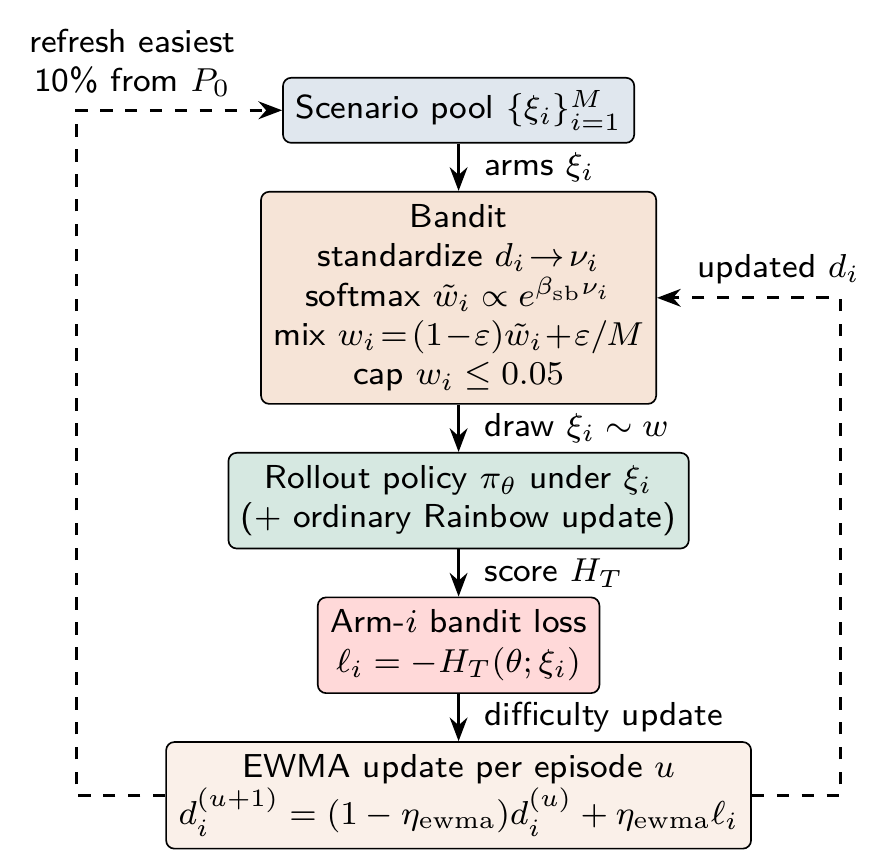
\includegraphics[width=0.5\linewidth]{scenario_bandit_diagram.png}
  \caption{The Algorithm~C scenario-bandit loop.  Pool difficulties $d_i$
  are converted into sampling probabilities $w_i$ by standardization,
  softmax reweighting, an $\varepsilon$-uniform mix, and a per-arm
  cap; a scenario $\xi_i \sim w$ is rolled out under the ordinary
  Rainbow/C51 update, its penalized terminal score $H_T$ defines the
  arm loss $\ell_i = -H_T(\theta;\xi_i)$, and the selected arm's
  difficulty is updated by the EWMA.  Dashed arrows mark the feedback
  paths: updated difficulties feed the next selection, and the easiest
  $10\%$ of the pool is periodically regenerated from $P_0$.}
  \label{fig:scenario_bandit_loop}
\end{figure}

\paragraph{Random-persistence bandit fine-tuning.}
Figure~\ref{fig:bandit_random_tau} compares the Algorithm~B controller
with the fine-tuned scenario-bandit controller under the random-$\tau$ stress. Relative to the Algorithm~B benchmark in this plot, scenario-bandit
fine-tuning improves mean terminal PnL by about $16\%$ and reduces
the empirical standard deviation to about $70\%$ of its Algorithm~B
level. 

\begin{figure}[htbp]
  \centering
  \begin{subfigure}[t]{0.48\textwidth}
    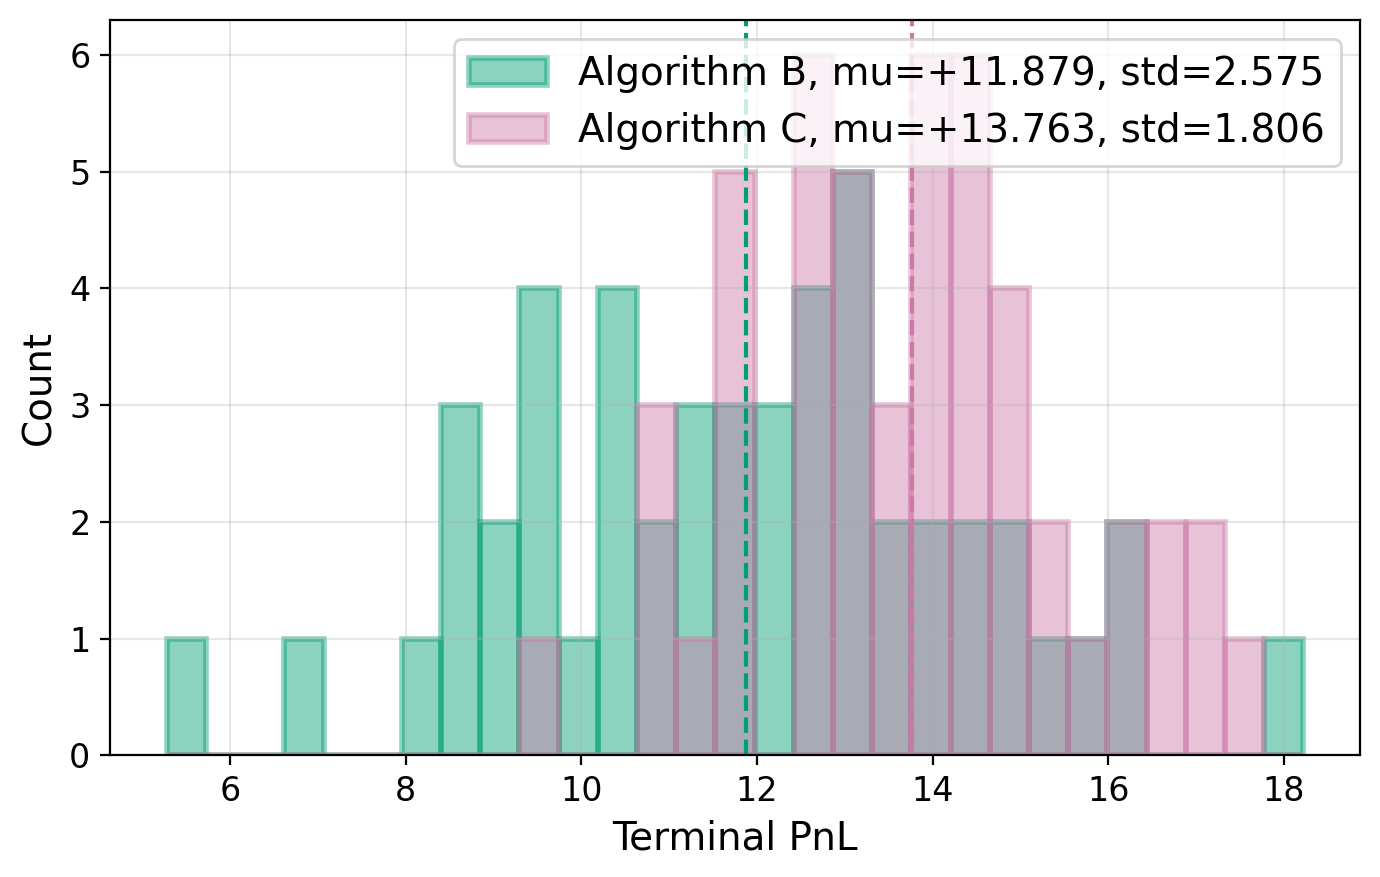
\includegraphics[width=\linewidth]{scenario_bandit_random_tau.png}
    \caption{Random-persistence stress: terminal-PnL distributions for
    the Algorithm~B (green) and Algorithm~C scenario-bandit (pink) controllers
    on the random-$\tau_{r}$ regimes.}
    \label{fig:bandit_random_tau}
  \end{subfigure}
  \hfill
  \begin{subfigure}[t]{0.48\textwidth}
    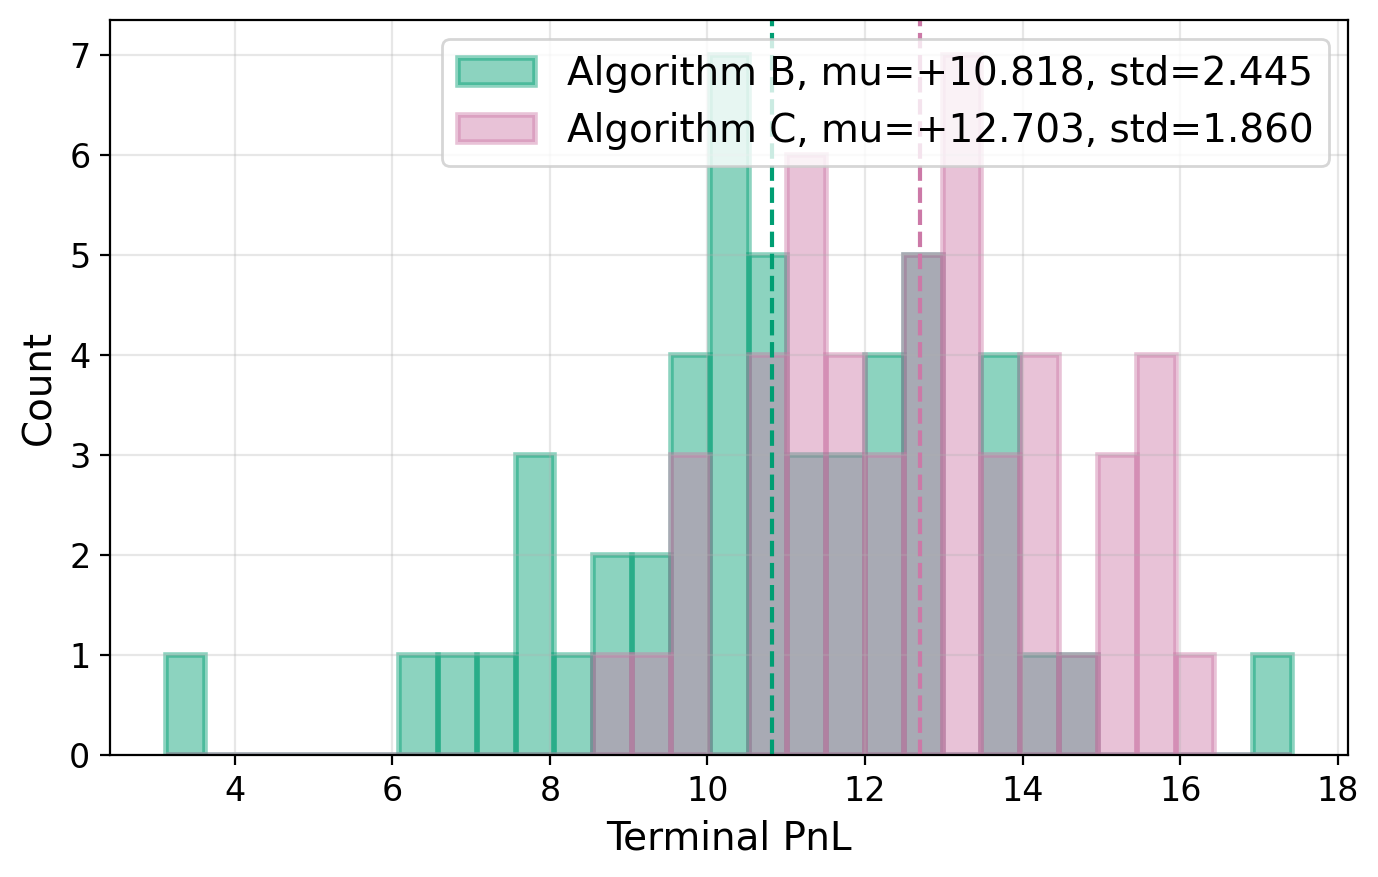
\includegraphics[width=\linewidth]{scenario_bandit_correlated_regime_stress.png}
    \caption{Correlated-direction stress: terminal-PnL distributions
    when regime signs persist across boundaries with probability
    $\rho_{\mathrm{side}}=0.85$.}
    \label{fig:bandit_correlated_regime_stress}
  \end{subfigure}
  \caption{Algorithm~C scenario-bandit fine-tuning under both stress
  families.  In each panel, ``Algorithm~C'' denotes the
  Algorithm~B controller after the scenario-bandit fine-tuning of
  Section~\ref{sec:scenario_bandit_finetuning}.}
  \label{fig:bandit_combined}
\end{figure}

\paragraph{Correlated-direction bandit fine-tuning.}
Correlated-direction stress is more adversarial because the sign
of the market-order imbalance persists across regime boundaries.
Relative to the stress benchmark of Algorithm~B in 
Figure~\ref{fig:bandit_correlated_regime_stress}, the adjustment of the scenario-bandit improves the mean terminal PnL by approximately $17\%$ and reduces the empirical standard deviation to approximately $76\%$ of its Algorithm~B
level. 

These two diagnostics clarify the role of the scenario bandit.
Algorithm~B learns to use belief and quote-exposure features to survive
non-stationary flow, but its training objective is still the average-case.
The bandit changes which stored regimes are replayed more often,
directing updates toward adverse realizations.
The result is an RLMM whose performance is less sensitive to
random regime persistence and more resilient to clustered directional
pressure.

\section{Discussion and Conclusion}

Our findings are threefold.  First, classical analytical control
remains a meaningful benchmark in realistic microstructure: GLFT,
once properly calibrated, transfers well to an event-driven
stochastic LOB and dominates the at-best baseline in risk--return terms.
Second, a
distributional DQN is a viable controller for market making and
outperforms GLFT over the entire observed stationary risk--return frontier,
showing that data-driven control can extract structure that
closed-form policies miss.  Third, robustness rather than raw
profitability is the central open problem: agents trained in a
stationary order-flow simulator are strongly unprofitable under
persistent directional flow, and this fragility is not resolved by
larger networks or more training data alone.

The fine-tuning pipeline introduced here provides a first concrete
answer: re-training the stationary-optimal controller on
regime-switching flow with a Bayesian change-point belief over
directional order flow and a queue-adjusted quote-exposure signal
recovers profitability under non-stationary order flow.  The scenario-bandit fine-tuning step
adds a second layer of robustness by upweighting the low-return regime
scenarios in the sampling distribution; in the
random-persistence and correlated-direction diagnostics it improves
the stressed terminal-PnL distribution without adding new state
information to the agent.

\paragraph{Limitations.}
Some limitations qualify these results.  (i)~All evaluations are based on simulated data: order flow is generated by a calibrated
zero-intelligence Santa Fe model rather than a more realistic LOB simulator
that includes strategic counterparts.  (ii)~The market maker quotes unit lots with at most one
resting order per side, so order sizing and multi-level quoting are out
of scope.  (iii)~The regime model fixes the width at $\omega = 0.30$
and uses exponential durations; richer regime structures (heavy-tailed
durations, more than two directional modes, intraday seasonality) are
not explored. 

\paragraph{Outlook.}
These limitations point to concrete next steps.  A first direction is
to move beyond the zero-intelligence simulator toward more realistic market models. A second is to enrich the action space with order sizing
and multi-level quoting and to add execution-cost and queue-position
features that the current compact state omits.

\paragraph{Conclusion.}
The central contribution is a two-stage fine-tuning
pipeline---a Bayesian regime belief with a queue-adjusted exposure
signal (Algorithm~B), followed by scenario-bandit reweighting
(Algorithm~C)---that turns a stationary-optimal RLMM into a
controller that remains profitable under regime-switching flow and has
a tighter stressed terminal-PnL tail.  

{\small
\bibliographystyle{unsrtnat}
\bibliography{references}
}

\appendix

\section{Bayesian Online Flow Filter}
\label{app:bayesian_flow_filter}

This appendix derives the Bayesian belief used in the Algorithm~B state
augmentation, adapting the Bayesian online change-point detection
framework of \citet{adams2007bocpd} (see also \citealp{fearnhead2007online})
to the signed market-order stream.  The filter is defined on the market-order clock: the
index $t$ below counts market orders rather than all LOB events.  At
the $t$-th market order the observed side is
\[
  y_t =
  \begin{cases}
    1, & \text{buy market order},\\
    0, & \text{sell market order}.
  \end{cases}
\]
The controller does not observe the simulator's latent regime labels,
regime ages, or buy probabilities; it observes only a posterior
summary inferred from the sequence $y_{1:t}$.

\subsection{Beta--Bernoulli Segment Model}

Within a fixed directional-flow segment, the market-order sides are
conditionally i.i.d.\ Bernoulli with probability $p$:
\[
  y_t\mid p \sim \mathrm{Bernoulli}(p).
\]
The directional bias associated with this segment is
\[
  \iota=2p-1,
\]
so that $\iota=0$ is balanced flow, $\iota>0$ is buy-heavy flow, and $\iota<0$
is sell-heavy flow.  A newly born segment starts from the Beta prior
\[
  p\sim\mathrm{Beta}(a_0,b_0),
  \qquad
  f_0(p)=
  \frac{p^{a_0-1}(1-p)^{b_0-1}}{\mathrm{B}(a_0,b_0)},
  \qquad 0<p<1,
\]
where
\[
  \mathrm{B}(a,b)=\int_0^1 u^{a-1}(1-u)^{b-1}\,du
\]
is the beta-function normalizer.  After observing $B$ buys and $S$
sells assigned to the same segment, conjugacy gives
\[
  p\mid y_{1:t},\text{segment}
  \sim
  \mathrm{Beta}(a_0+B,b_0+S).
\]
Writing $a=a_0+B$ and $b=b_0+S$, the posterior mean is
\[
  \mu(a,b)=\E[p\mid a,b]=\frac{a}{a+b}.
\]
The one-step predictive probability of a new market-order side,
after integrating out $p$, is
\begin{align}
  \Prob(y\mid a,b)
  &=
  \int_0^1 p^y(1-p)^{1-y}
  \frac{p^{a-1}(1-p)^{b-1}}{\mathrm{B}(a,b)}\,dp \notag\\
  &=
  \frac{\mathrm{B}(a+y,b+1-y)}{\mathrm{B}(a,b)}.
\end{align}
Thus
\[
  \Prob(y=1\mid a,b)=\frac{a}{a+b},
  \qquad
  \Prob(y=0\mid a,b)=\frac{b}{a+b}.
\]
These predictive probabilities are the local evidence terms used by
the change-point recursion.

\subsection{Run-Length Filtering}

Let $\ell_t$ denote the number of market orders since the current
directional-flow segment began.  The Bayesian online change-point
filter maintains
\[
  g_t(\ell)=\Prob(\ell_t=\ell\mid y_{1:t}),
\]
together with a Beta posterior
\[
  p\mid \ell_t=\ell,y_{1:t}
  \sim
  \mathrm{Beta}\bigl(a_t^{(\ell)},b_t^{(\ell)}\bigr)
\]
for each active run-length hypothesis.  A run-length hypothesis is
therefore a joint statement about the age of the current segment and
the buy/sell evidence accumulated inside that candidate segment.

For a single characteristic regime duration $\tau_r$, the constant
per-event reset hazard from the $\mathrm{Exp}(1/\tau_r)$ duration is
\[
  h = 1-\exp(-1/\tau_r).
\]
Before the next market order, the probability $1-h$ is assigned to
continuation of the current segment and the probability $h$ to a reset.

Consider a previous run length $\ell$ at time $t-1$.  Its posterior mean
buy probability is
\[
  \mu_{t-1}^{(\ell)}
  =
  \frac{a_{t-1}^{(\ell)}}{a_{t-1}^{(\ell)}+b_{t-1}^{(\ell)}}.
\]
The predictive probability of the new side $y_t$ under this
continuation hypothesis is
\[
  \mathcal{E}_t^{(\ell)}
  =
  \begin{cases}
    \mu_{t-1}^{(\ell)}, & y_t=1,\\
    1-\mu_{t-1}^{(\ell)}, & y_t=0.
  \end{cases}
\]
The unnormalized continuation mass is then
\[
  \widetilde g_t(\ell+1)
  =
  g_{t-1}(\ell)(1-h)\mathcal{E}_t^{(\ell)},
\]
and the corresponding Beta parameters absorb the new Bernoulli
observation,
\[
  a_t^{(\ell+1)}=a_{t-1}^{(\ell)}+y_t,
  \qquad
  b_t^{(\ell+1)}=b_{t-1}^{(\ell)}+1-y_t.
\]

The change-point branch pools the reset mass from all previous
run-length hypotheses, with $y_t$ scored as the first datum of the new
segment.  A fresh segment uses the prior predictive
probability
\[
  \mathcal{E}_t^{(0)}
  =
  \begin{cases}
    a_0/(a_0+b_0), & y_t=1,\\
    b_0/(a_0+b_0), & y_t=0.
  \end{cases}
\]
Hence,
\[
  \widetilde g_t(1)
  =
  \mathcal{E}_t^{(0)}
  \sum_\ell g_{t-1}(\ell)h.
\]
Under the above constant hazard, the sum equals $h$ because
$\sum_{\ell\ge1} g_{t-1}(\ell)=1$ (all run-length sums range over $\ell\ge1$). The posterior parameters of the fresh segment are
\[
  a_t^{(1)}=a_0+y_t,
  \qquad
  b_t^{(1)}=b_0+1-y_t.
\]

The continuation and change-point branches are normalized by
\[
  Z_t=\sum_\ell \widetilde g_t(\ell),
  \qquad
  g_t(\ell)=\frac{\widetilde g_t(\ell)}{Z_t}.
\]
The normalization constant is the Bayesian predictive likelihood
$\Prob(y_t\mid y_{1:t-1})$. The large posterior mass on small run
lengths therefore corresponds to evidence that the directional-flow
segment has recently changed.

\subsection{Belief Summary Supplied to the Controller}

The Algorithm~B controller receives a low-dimensional summary of the
posterior distribution.  First, the run-length posterior is used to
average the posterior buy probability:
\[
  \widehat p_t
  =
  \sum_\ell g_t(\ell)
  \frac{a_t^{(\ell)}}{a_t^{(\ell)}+b_t^{(\ell)}}.
\]
The signed Bayesian flow estimate is
\[
  \widehat{\iota}_t = 2\widehat p_t-1.
\]
Second, the posterior expected run length is
\[
  \bar{\ell}_t
  =
  \sum_\ell g_t(\ell)\,\ell.
\]
The belief vector used in the Algorithm~B state is therefore
\[
  b_t=(\widehat{\iota}_t,\bar{\ell}_t).
\]
This pair separates direction from persistence: $\widehat{\iota}_t$
summarizes the inferred side of the current flow pressure, while
$\bar{\ell}_t$ summarizes how old the current directional episode
appears to be.

\section{Closed-Form GLFT Misspecification Under Flow Asymmetry}
\label{app:glft_misspecification}

This appendix derives the analytical curve used in
Figure~\ref{fig:misspec_comparison}.  The object is a GLFT market
maker whose quotes are computed under a symmetric order flow, but whose
realized fills are generated by a static asymmetric market-order
environment with buy probability $p\in(0,1)$.  The parameter $p$ remains
 fixed throughout the episode.  The analysis therefore isolates
directional misspecification from regime persistence.

\subsection{Misspecified GLFT Quotes and True Fill Rates}

All quantities used in this appendix are expressed in ticks and in the
same time units as the calibrated fill intensities.  The GLFT policy is
computed under the symmetric-flow model and then evaluated under a
true static buy-MO probability $p$.  The policy therefore uses a
single quote map for every $p$; only the side-specific fill
rates realized change with $p$.

Let $q\in\{-Q,\ldots,Q\}$ be an inventory, where $Q = q_{\max}$ is the hard
inventory cap of the main text (we keep the compact symbol $Q$ within
this appendix; it is not related to the action value $Q_\theta$).  Under the GLFT coefficients of
Equations~\eqref{eq:glft_ask}--\eqref{eq:glft_bid}, define the
baseline half-spread
\[
  \delta_{\mathrm{base}}
  =
  \frac{1}{\gamma_{\mathrm{GLFT}}}
  \log\!\left(1+\frac{\gamma_{\mathrm{GLFT}}}{\kappa}\right),
\]
and the inventory-skew coefficient;
\[
  c_{\mathrm{skew}}
  =
  \sqrt{
    \frac{\sigma^2\gamma_{\mathrm{GLFT}}}{2\kappa A}
    \left(1+\frac{\gamma_{\mathrm{GLFT}}}{\kappa}\right)^{1+\kappa/\gamma_{\mathrm{GLFT}}}
  }.
\]
Here $A$ and $\kappa$ are the exponential fill-intensity parameters,
$\sigma$ is the diffusion scale, and $\gamma_{\mathrm{GLFT}}$ is the GLFT
risk-aversion parameter.  At zero inventory, the continuous GLFT quote
distance is
\[
  \bar\delta
  =
  \delta_{\mathrm{base}}+\frac{c_{\mathrm{skew}}}{2}.
\]
For inventory $q$, the signal-blind GLFT policy posts continuous
distances from the mid
\[
  \delta_a(q)=\bar\delta-c_{\mathrm{skew}}q,
  \qquad
  \delta_b(q)=\bar\delta+c_{\mathrm{skew}}q,
\]
where $\delta_a$ is the ask distance and $\delta_b$ is the bid
distance.

The realized environment has total market-order intensity fixed, but
splits that flow according to the buy probability $p$. In
the ideal GLFT model, a quote at distance $\delta$ has fill intensity
$A e^{-\kappa\delta}$.  In the FIFO simulator, however, the agent
shares queues with other resting orders and can lose priority through
discrete decision updates.  We therefore use the effective scale
\[
  A_{\mathrm{eff}}=\eta A,
  \qquad
  \eta
  =
  \frac{R_{\mathrm{empirical}}}
       {2A e^{-\kappa\bar\delta}},
\]
where $R_{\mathrm{empirical}}$ is the empirical two-sided fill rate of
the simulator at symmetric flow, measured at the zero-inventory quote
depth $\bar\delta$.  Operationally, if
$N_{e}^{a,\mathrm{fill}}(\bar\delta)$ and
$N_{e}^{b,\mathrm{fill}}(\bar\delta)$ are the ask- and bid-side fills
observed in symmetric-flow calibration episode $e$, with
$e=1,\ldots,E_{\mathrm{calib}}$, and $T_e$ is the corresponding
episode exposure time, then
\[
  R_{\mathrm{empirical}}
  =
  \frac{
    \sum_{e=1}^{E_{\mathrm{calib}}}
    \left[
      N_{e}^{a,\mathrm{fill}}(\bar\delta)
      +
      N_{e}^{b,\mathrm{fill}}(\bar\delta)
    \right]
  }{
    \sum_{e=1}^{E_{\mathrm{calib}}} T_e
  }.
\]
The denominator $2A e^{-\kappa\bar\delta}$ is the corresponding
two-sided GLFT prediction at $p=1/2$.  With this convention, the
realized interior fill rates under a true buy-MO probability $p$ are
\begin{align}
  r_a(q;p)
  &=
  2p\,A_{\mathrm{eff}}e^{-\kappa\delta_a(q)}
  =
  2A_{\mathrm{eff}}e^{-\kappa\bar\delta}
  p\,e^{\kappa c_{\mathrm{skew}}q},
  \label{eq:app_miss_ra}\\
  r_b(q;p)
  &=
  2(1-p)\,A_{\mathrm{eff}}e^{-\kappa\delta_b(q)}
  =
  2A_{\mathrm{eff}}e^{-\kappa\bar\delta}
  (1-p)e^{-\kappa c_{\mathrm{skew}}q}.
  \label{eq:app_miss_rb}
\end{align}
The factors $2p$ and $2(1-p)$ keep the total market-order intensity
fixed while changing only the side split.  At $p=1/2$ both factors
equal one, so $r_a(q;1/2)=A_{\mathrm{eff}}e^{-\kappa\delta_a(q)}$ and
$r_b(q;1/2)=A_{\mathrm{eff}}e^{-\kappa\delta_b(q)}$ recover the
symmetric effective intensities.
The hard inventory cap is enforced by setting
\[
  r_a(-Q;p)=0,
  \qquad
  r_b(Q;p)=0.
\]
Thus the boundary state $-Q$ cannot receive another ask fill, and the
boundary state $Q$ cannot receive another bid fill.

The numerical curves in Figure~\ref{fig:misspec_comparison} and in
the appendix diagnostics use the calibrated values of
Eq.~\eqref{eq:glft_calib_values},
\[
  A=0.1507,\qquad
  \kappa=2.335,\qquad
  \sigma=0.30,\qquad
  \gamma_{\mathrm{GLFT}}=10^{-6},\qquad
  Q=8,\qquad
  \eta\simeq0.82 .
\]
These values give
$\delta_{\mathrm{base}}\simeq0.43$ ticks and
$c_{\mathrm{skew}}\simeq5.90\times10^{-4}$, hence
$\bar\delta\simeq0.43$ ticks.  In the PnL expressions below, $T$
denotes the episode duration in the same time units as the rates
(distinct from the decision count $T$ of
Section~\ref{sec:scenario_bandit_finetuning}), and
$v_{\mathrm{tick}}$ is the monetary value of one tick; the plotted
curves use $v_{\mathrm{tick}}=1$.

\subsection{Stationary Inventory Distribution}

The inventory process is a finite continuous-time birth--death chain.
A bid fill moves $q\mapsto q+1$ at rate $r_b(q;p)$, and an ask fill
moves $q\mapsto q-1$ at rate $r_a(q;p)$.  Let $\psi(q)$ denote the
stationary probability of inventory state $q$.  For an interior state,
the stationary Kolmogorov forward equation is
\[
  0
  =
  \psi(q-1)r_b(q-1;p)
  +
  \psi(q+1)r_a(q+1;p)
  -
  \psi(q)\bigl[r_b(q;p)+r_a(q;p)\bigr],
  \qquad -Q<q<Q.
\]
This equation says that, in stationarity, probability flow into state
$q$ equals probability flow out of state $q$.  Equivalently, define the
net probability current across the edge between $q$ and $q+1$ as
\[
  J_q
  =
  \psi(q)r_b(q;p)
  -
  \psi(q+1)r_a(q+1;p),
  \qquad q=-Q,\ldots,Q-1.
\]
The stationary equation above is then $J_{q-1}=J_q$: the current must
be constant across all adjacent inventory edges.  Because the hard
inventory cap gives $r_a(-Q;p)=0$ and $r_b(Q;p)=0$, global balance at
$-Q$ reads $\psi(-Q)r_b(-Q)=\psi(-Q+1)r_a(-Q+1)$, i.e.\ $J_{-Q}=0$;
constancy of the current then forces $J_q=0$ for every edge.  This zero-current condition is
the detailed-balance equation,
\[
  \psi(q)r_b(q;p)=\psi(q+1)r_a(q+1;p),
  \qquad q=-Q,\ldots,Q-1.
\]
For $q=0,\ldots,Q-1$, substituting
\eqref{eq:app_miss_ra}--\eqref{eq:app_miss_rb} gives
\[
  \frac{\psi(q+1)}{\psi(q)}
  =
  \frac{r_b(q;p)}{r_a(q+1;p)}
  =
  \frac{1-p}{p}\,
  e^{-\kappa c_{\mathrm{skew}}(2q+1)}.
\]
The positive-inventory side is obtained by iterating this adjacent
ratio from the reference state $q=0$:
\begin{align}
  \frac{\psi(q)}{\psi(0)}
  &=
  \prod_{j=0}^{q-1}
  \frac{\psi(j+1)}{\psi(j)} \notag\\
  &=
  \prod_{j=0}^{q-1}
  \left[
    \frac{1-p}{p}\,
    e^{-\kappa c_{\mathrm{skew}}(2j+1)}
  \right] \notag\\
  &=
  \left(\frac{1-p}{p}\right)^q
  \exp\!\left\{
    -\kappa c_{\mathrm{skew}}
    \sum_{j=0}^{q-1}(2j+1)
  \right\} \notag\\
  &=
  \left(\frac{1-p}{p}\right)^q
  e^{-\kappa c_{\mathrm{skew}}q^2},
  \qquad q=1,\ldots,Q,
\end{align}
where the last equality uses
$\sum_{j=0}^{q-1}(2j+1)=q^2$.  Hence
\[
  \psi(q)
  =
  \psi(0)
  \left(\frac{1-p}{p}\right)^q
  e^{-\kappa c_{\mathrm{skew}}q^2},
  \qquad q=1,\ldots,Q.
\]
The negative side is obtained by the same argument, iterating the
detailed-balance ratios backwards from zero.  Writing $q=-m$ with
$m>0$ gives
\[
  \psi(-m)
  =
  \psi(0)
  \left(\frac{p}{1-p}\right)^m
  e^{-\kappa c_{\mathrm{skew}}m^2}.
\]
Define the logit asymmetry
\[
  \vartheta=\log\left(\frac{p}{1-p}\right).
\]
Then the positive branch can be rewritten as
\[
  \frac{\psi(q)}{\psi(0)}
  =
  \left(\frac{1-p}{p}\right)^q
  e^{-\kappa c_{\mathrm{skew}}q^2}
  =
  e^{-\vartheta q}
  e^{-\kappa c_{\mathrm{skew}}q^2},
  \qquad q=1,\ldots,Q,
\]
while on the negative branch, with $q=-m$,
\[
  \frac{\psi(q)}{\psi(0)}
  =
  \left(\frac{p}{1-p}\right)^{-q}
  e^{-\kappa c_{\mathrm{skew}}q^2}
  =
  e^{\vartheta(-q)}
  e^{-\kappa c_{\mathrm{skew}}q^2}
  =
  e^{-\vartheta q}
  e^{-\kappa c_{\mathrm{skew}}q^2},
  \qquad q=-Q,\ldots,-1.
\]
The same expression also holds at $q=0$, because both exponentials are
then equal to one.  Hence, for every admissible inventory state,
\[
  \psi(q)
  =
  \psi(0)
  \exp\{-\kappa c_{\mathrm{skew}}q^2-\vartheta q\},
  \qquad q=-Q,\ldots,Q.
\]
At this stage $\psi(0)$ is still an unknown multiplicative constant.
It is determined by the normalization condition
\[
  1
  =
  \sum_{q=-Q}^{Q}\psi(q)
  =
  \psi(0)
  \sum_{q=-Q}^{Q}
  \exp\{-\kappa c_{\mathrm{skew}}q^2-\vartheta q\}.
\]
Therefore
\[
  \psi(0)
  =
  \left[
    \sum_{q=-Q}^{Q}
    \exp\{-\kappa c_{\mathrm{skew}}q^2-\vartheta q\}
  \right]^{-1}.
\]
Writing this normalizing denominator as $Z(\vartheta)$ gives the tilted
discrete Gaussian
\begin{equation}
  \psi(q)
  =
  \frac{1}{Z(\vartheta)}
  \exp\{-\kappa c_{\mathrm{skew}} q^2-\vartheta q\},
  \qquad
  Z(\vartheta)
  =
  \sum_{n=-Q}^{Q}\exp\{-\kappa c_{\mathrm{skew}} n^2-\vartheta n\}.
  \label{eq:app_miss_pi}
\end{equation}
The stationary law $\psi(q)$ is a discrete truncated analog
of a Gaussian: the inventory-skew term
$\exp\{-\kappa c_{\mathrm{skew}}q^2\}$ penalizes large absolute
inventories symmetrically around zero, and the flow asymmetry enters only
through the linear tilt $\exp\{-\vartheta q\}$, with
$\vartheta=\log(p/(1-p))$.  When $p=1/2$, $\vartheta=0$ and the tilt
vanishes, so the law is symmetric around zero inventory.
When $p>1/2$, $\vartheta>0$: positive inventories are down-weighted by
$e^{-\vartheta q}$, while negative inventories are up-weighted because
$-\vartheta q>0$ for $q<0$.  Thus buy-heavy flow shifts stationary mass
toward short inventory, reflecting the fact that buy market orders
hit the market maker's ask quotes and therefore sell inventory out of
the book.  Conversely, when $p<1/2$, the tilt has the opposite sign
and the distribution shifts toward long inventory
(Figure~\ref{fig:app_miss_stationary_law}).

\begin{figure}[htbp]
  \centering
  \begin{subfigure}[b]{0.50\linewidth}
    \centering
    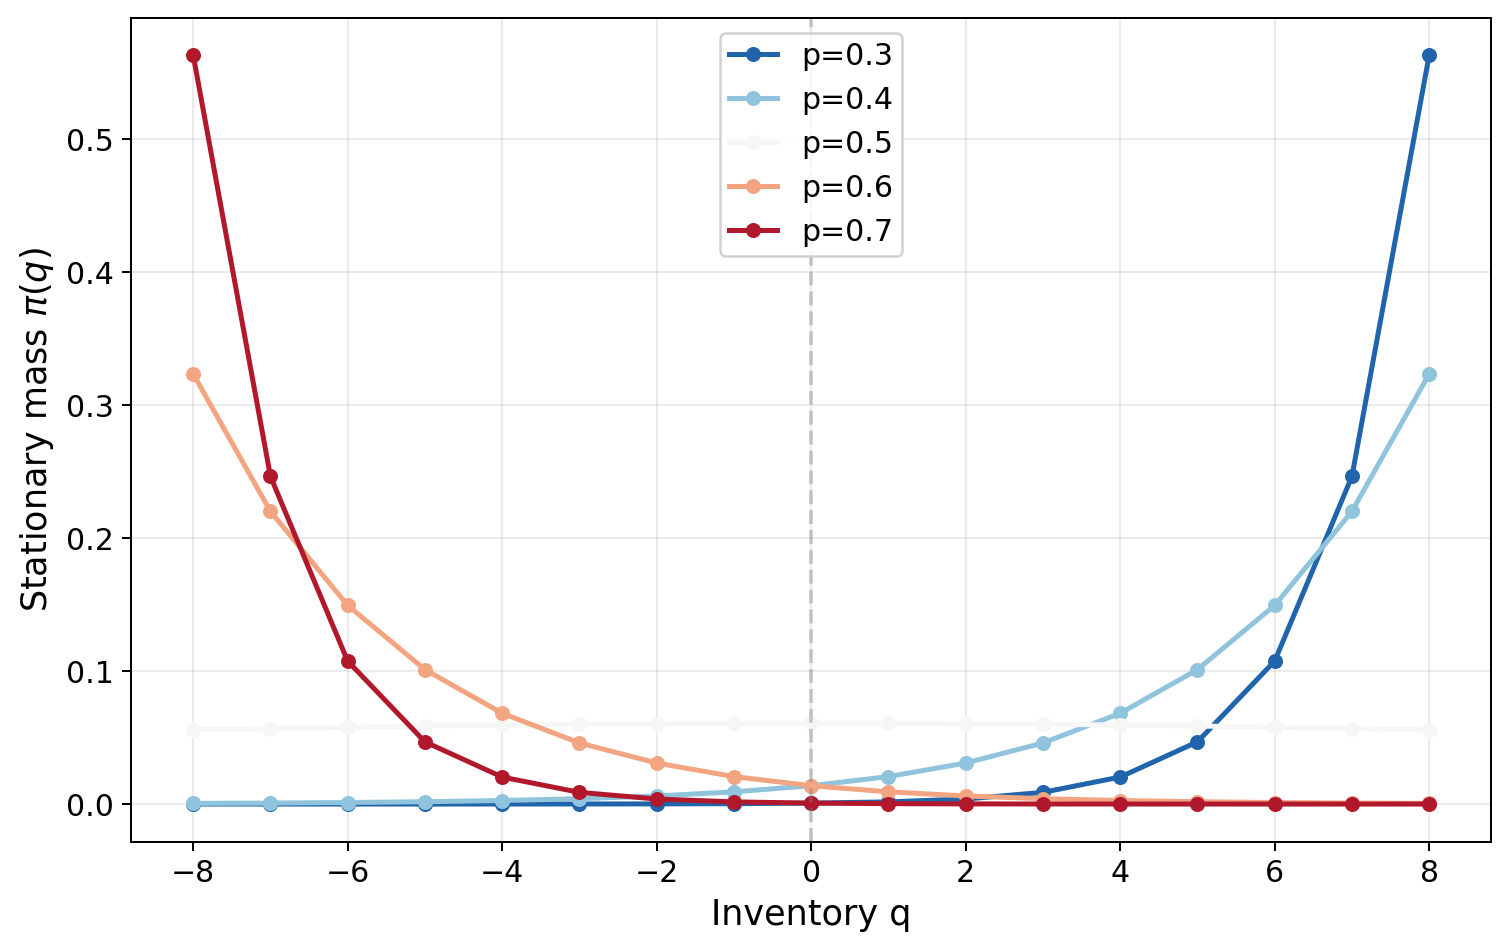
\includegraphics[width=\linewidth]{as_miss_pi_q_lines.png}
    \caption{Selected $p$ values.}
    \label{fig:app_miss_pi_lines}
  \end{subfigure}%
  \begin{subfigure}[b]{0.50\linewidth}
    \centering
    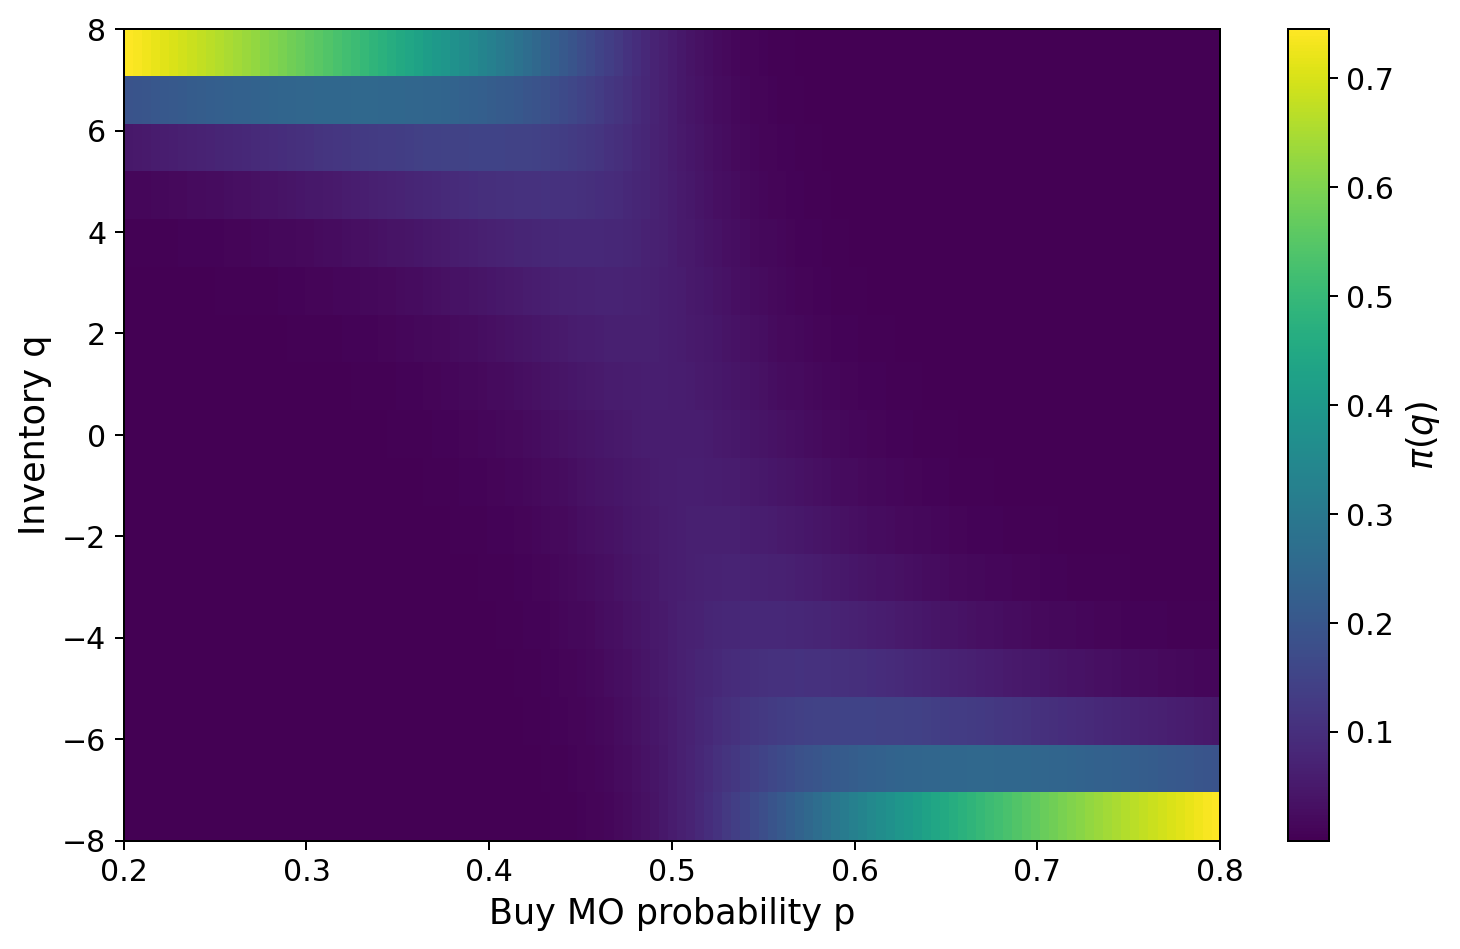
\includegraphics[width=\linewidth]{as_miss_pi_heatmap.png}
    \caption{Full $p$ range.}
    \label{fig:app_miss_pi_heatmap}
  \end{subfigure}
  \caption{Stationary inventory distribution under GLFT
  misspecification.  Flow asymmetry exponentially tilts the symmetric
  GLFT inventory law toward one inventory boundary.}
  \label{fig:app_miss_stationary_law}
\end{figure}

\subsection{Inventory Mean and Boundary Concentration}

The stationary mean inventory is

\[
  \bar q(p)=\sum_{q=-Q}^{Q}q\,\psi(q).
\]
To connect this mean to the normalizing constant, differentiate the partition function $Z(\vartheta)$ in \eqref{eq:app_miss_pi}.  Since
$\vartheta$ enters only through the linear term $-\vartheta n$,
\begin{align}
  \frac{\partial Z}{\partial\vartheta}
  &=
  \sum_{n=-Q}^{Q}
  (-n)\exp\{-\kappa c_{\mathrm{skew}}n^2-\vartheta n\} \notag\\
  &=
  -Z(\vartheta)
  \sum_{n=-Q}^{Q}
  n\,
  \frac{
    \exp\{-\kappa c_{\mathrm{skew}}n^2-\vartheta n\}
  }{
    Z(\vartheta)
  } \notag\\
  &=
  -Z(\vartheta)\sum_{n=-Q}^{Q} n\,\psi(n)
  =
  -Z(\vartheta)\bar q(p).
\end{align}
Dividing by $Z(\vartheta)$ gives
\begin{equation}
  \frac{\partial}{\partial\vartheta}\log Z(\vartheta)
  =
  \frac{1}{Z(\vartheta)}
  \frac{\partial Z}{\partial\vartheta}
  =
  -\bar q(p),
  \qquad\text{so}\qquad
  \bar q(p)
  =
  -\frac{\partial}{\partial\vartheta}\log Z(\vartheta).
  \label{eq:app_miss_qbar}
\end{equation}
The function $\bar q(p)$ is antisymmetric around $p=1/2$ (since $Z$ is even in $\vartheta$, so $\bar q=-\partial_\vartheta\log Z$ is odd).  This
anti-symmetry is the inventory mechanism behind the PnL loss under
directional flow: a buy-heavy environment pushes the market maker
short, while a sell-heavy environment pushes it long.  As the flow
becomes more asymmetric, stationary mass also moves toward the hard
inventory boundaries, where one side of the quote is disabled
(Figure~\ref{fig:app_miss_inventory_diagnostics}).

\begin{figure}[htbp]
  \centering
  \begin{subfigure}[b]{0.50\linewidth}
    \centering
    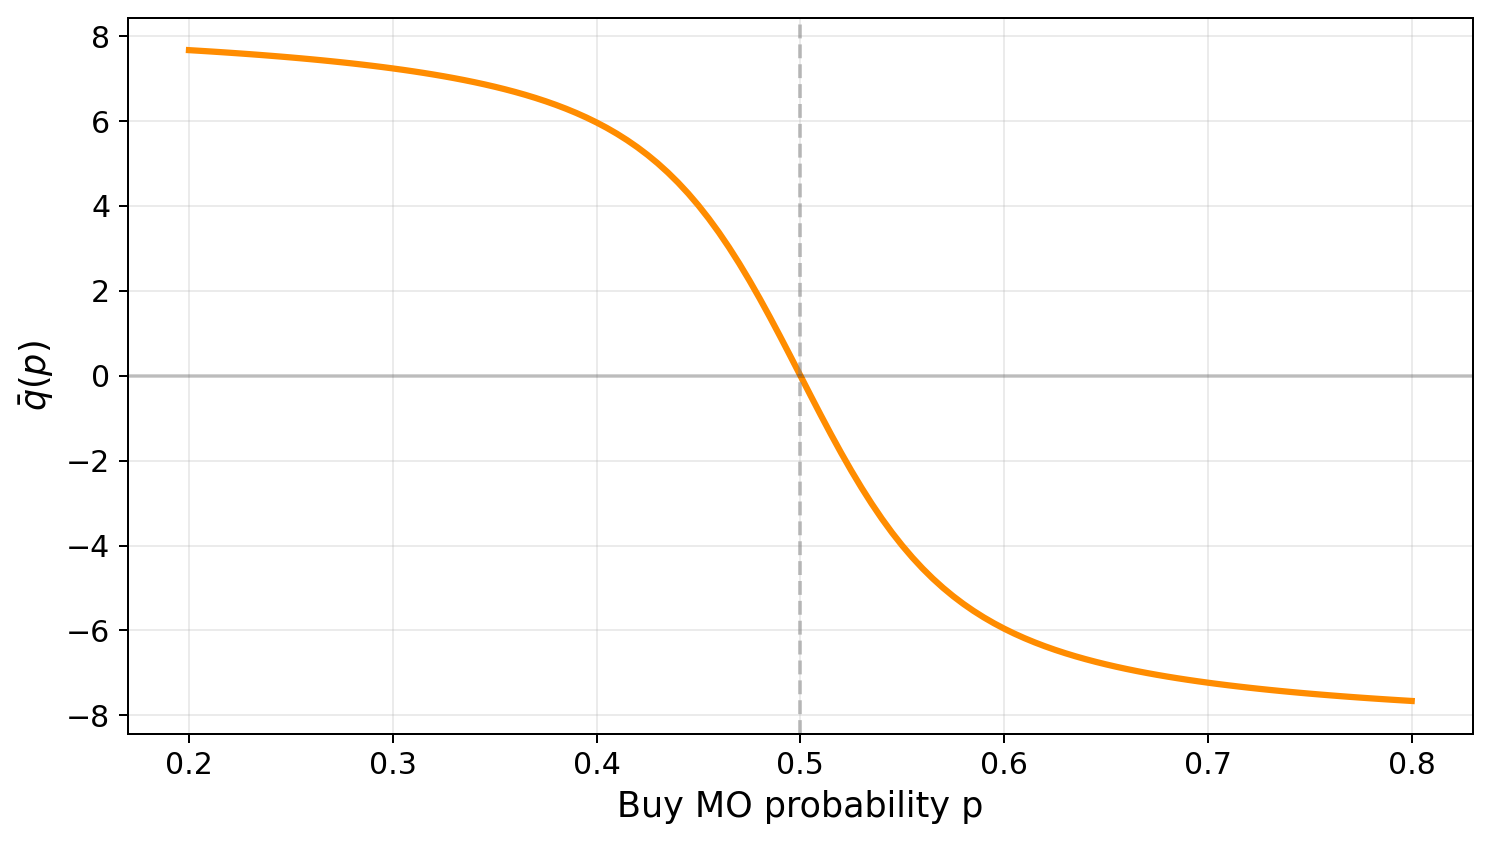
\includegraphics[width=\linewidth]{as_miss_qbar_vs_p.png}
    \caption{Expected inventory.}
    \label{fig:app_miss_qbar}
  \end{subfigure}%
  \begin{subfigure}[b]{0.50\linewidth}
    \centering
    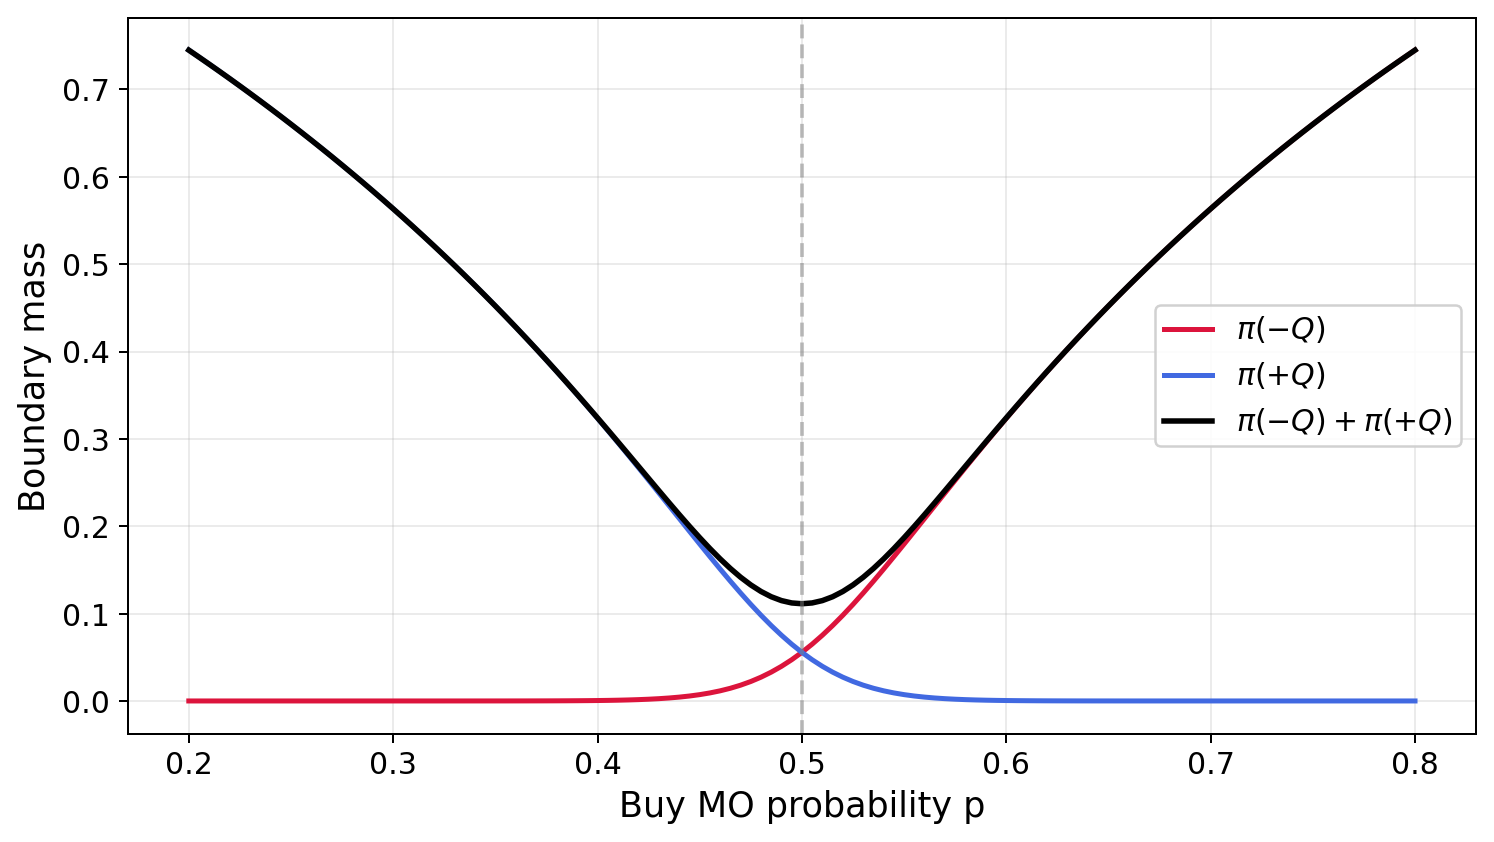
\includegraphics[width=\linewidth]{as_miss_boundary_mass_vs_p.png}
    \caption{Boundary mass.}
    \label{fig:app_miss_boundary}
  \end{subfigure}
  \caption{Inventory bias and boundary concentration induced by
  static flow asymmetry.  The inventory mean is antisymmetric around
  $p=1/2$, while the total mass at $\pm Q$ increases as the flow
  becomes more one-sided.}
  \label{fig:app_miss_inventory_diagnostics}
\end{figure}

\subsection{Expected Spread Capture}

At inventory $q$, the instantaneous expected spread-capture rate is
\[
  g(q;p)
  =
  r_a(q;p)\delta_a(q)+r_b(q;p)\delta_b(q),
\]
with the boundary convention $r_a(-Q;p)=0$ and $r_b(Q;p)=0$.  The
stationary expected spread-capture rate is therefore
\[
  \mathcal S(p)
  =
  \sum_{q=-Q}^{Q}\psi(q)g(q;p).
\]
Over an episode of duration $T$ and tick value $v_{\mathrm{tick}}$,
\begin{equation}
  \E[\mathrm{PnL}_{\mathrm{spread}}](p)
  =
  v_{\mathrm{tick}}T
  \sum_{q=-Q}^{Q}
  \psi(q)
  \bigl[
    r_a(q;p)\delta_a(q)+r_b(q;p)\delta_b(q)
  \bigr].
  \label{eq:app_miss_spread_pnl}
\end{equation}
This is the GLFT-consistent expected-PnL expression under the original
martingale mid-price assumption.  Indeed, if
\[
  \dd S_t=\sigma\,\dd W_t
\]
and the fill processes are independent of the Brownian increments,
the bounded inventory $|q_t|\le Q$ makes the running mark-to-market
contribution a martingale with zero expectation:
\[
  \E\left[\int_0^T q_t\,\dd S_t\right]=0.
\]
Within the original GLFT price model, expected PnL therefore reduces
to the spread-capture expression \eqref{eq:app_miss_spread_pnl}.

\subsection{Drift-Corrected Curve}

Persistent directional flow can also move the reference price.  A
first-order reduced form is
\[
  \dd S_t=v_0(2p-1)\,\dd t+\sigma\,\dd W_t,
\]
where $2p-1\in[-1,1]$ is the signed market-order imbalance
($-1$ for all sell MOs, $0$ for symmetric flow, and $+1$ for all buy
MOs), and $v_0>0$ converts this imbalance into expected mid-price
drift.  This drift term is not part of the original GLFT martingale
benchmark; it is an optional reduced-form correction used to visualize
the adverse mark-to-market effect of directional flow.  Setting
$v_0=0$ recovers the spread-only martingale curve of
Equation~\eqref{eq:app_miss_spread_pnl}.

We calibrate $v_0$ offline from static-asymmetry simulator runs.  For
each grid value $p_j$, we run several bare-LOB episodes with fixed buy
probability $p_j$ and measure the realized mid-price drift in episode
$e$ as
\[
  \widehat b_{j,e}
  =
  \frac{S_T^{(j,e)}-S_0^{(j,e)}}{T_{j,e}}.
\]
The episode drifts are averaged within each probability level,
\[
  \bar b_j
  =
  \frac{1}{E_j}\sum_{e=1}^{E_j}\widehat b_{j,e},
\]
and the reduced-form coefficient is then the zero-intercept
least-squares slope of this average realized drift on signed
imbalance,
\[
  \widehat v_0
  =
  \frac{\sum_j (2p_j-1)\bar b_j}
       {\sum_j (2p_j-1)^2}.
\]
Because every probability level $p_j$ uses the same number of
episodes $E_j$, this slope coincides with the slope from a pooled
regression on all individual episode drifts $\widehat b_{j,e}$.
Using the calibrated Santa Fe simulator gives
$\widehat v_0\approx0.05$ ticks per unit time.  The horizon $T$ is not
averaged over the $v_0$-calibration episodes.  Instead, it is measured
once from a separate symmetric bare-LOB episode whose event horizon
matches the analytical comparison, via
\[
  T = t_{\mathrm{last}}-t_{\mathrm{first}},
\]
which gives $T\approx 844$ simulated time units for the run used in
the plots.
Then
\[
  \E\left[\int_0^T q_t\,\dd S_t\right]
  =
  v_0(2p-1)T\,\bar q(p),
\]
and the full drift-corrected expected PnL is
\begin{equation}
  \E[\mathrm{PnL}_{\mathrm{full}}](p)
  =
  \E[\mathrm{PnL}_{\mathrm{spread}}](p)
  +
  v_{\mathrm{tick}}v_0(2p-1)T\,\bar q(p).
\end{equation}
For $p>1/2$, the drift is positive while
\eqref{eq:app_miss_qbar} gives $\bar q(p)<0$; for $p<1/2$, the
signs reverse.  Hence the drift correction is adverse on both sides
of the symmetric point (Figure~\ref{fig:app_miss_pnl}).

\begin{figure}[htbp]
  \centering
  \begin{subfigure}[b]{0.50\linewidth}
    \centering
    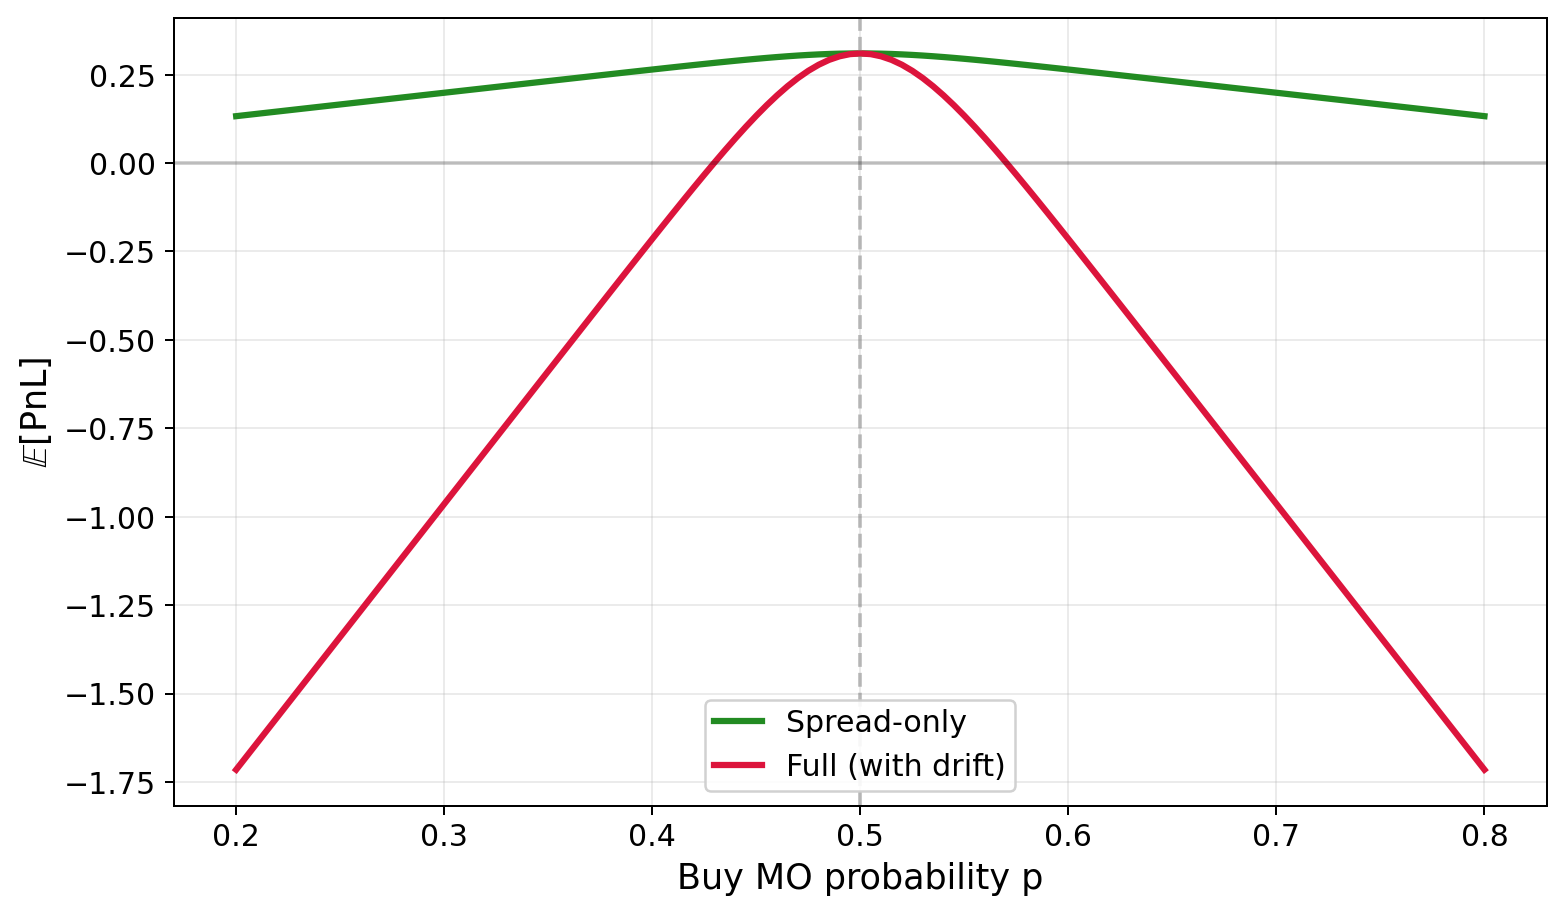
\includegraphics[width=\linewidth]{as_miss_expected_pnl_curves.png}
    \caption{Expected PnL curves.}
    \label{fig:app_miss_pnl_curves}
  \end{subfigure}%
  \begin{subfigure}[b]{0.50\linewidth}
    \centering
    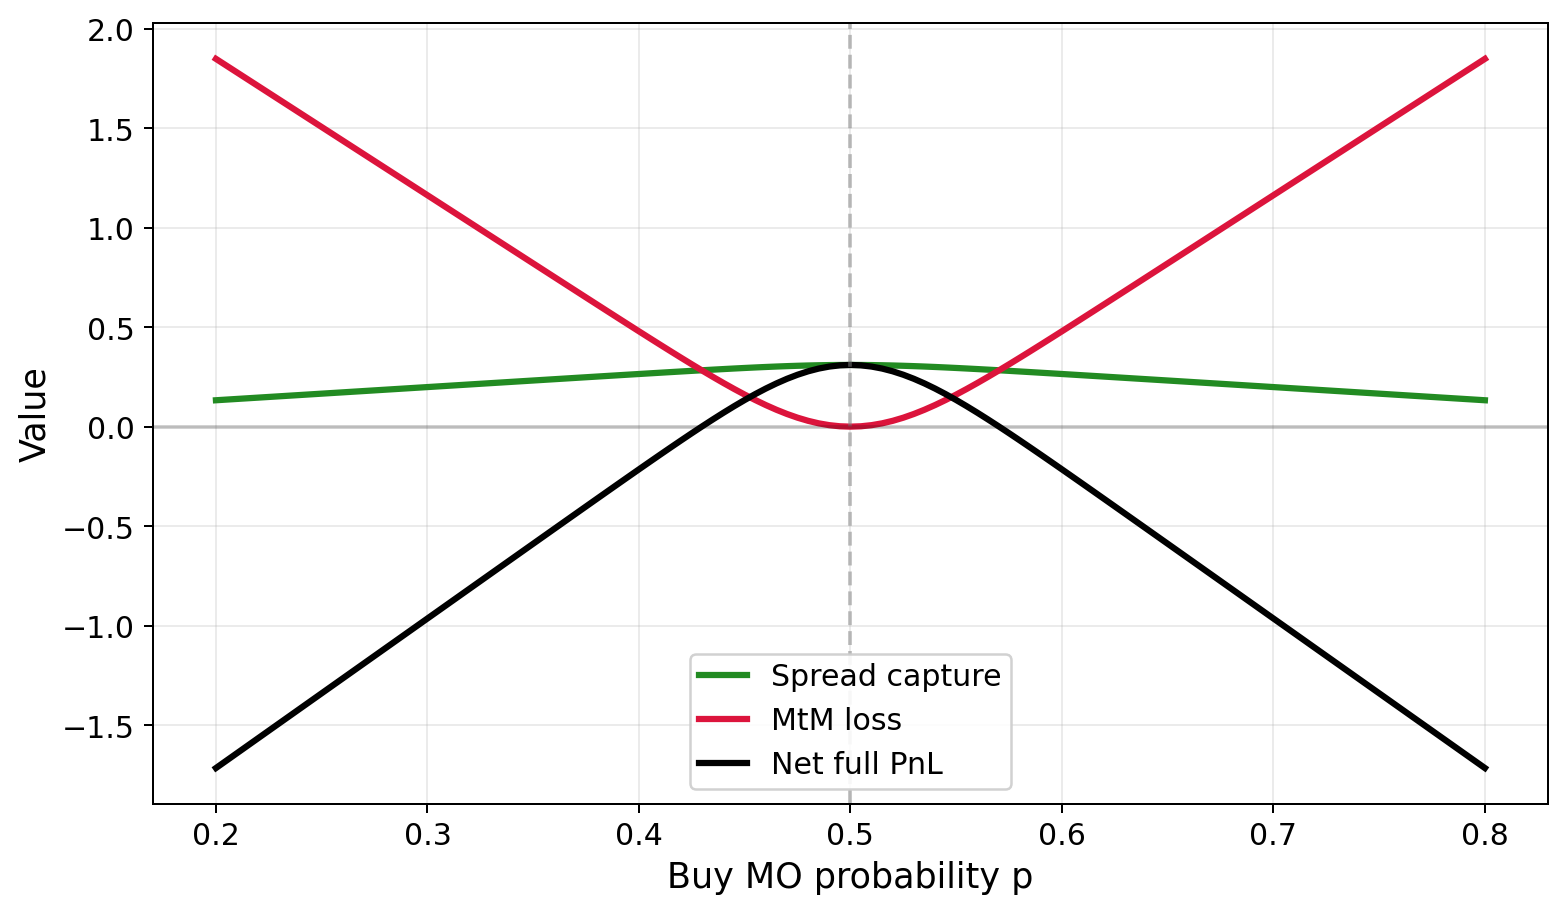
\includegraphics[width=\linewidth]{as_miss_pnl_decomposition.png}
    \caption{PnL decomposition.}
    \label{fig:app_miss_pnl_decomp}
  \end{subfigure}
  \caption{Expected PnL under static flow misspecification.  The
  spread-only curve is already damaged by boundary concentration, and
  the drift-corrected curve adds the adverse mark-to-market component
  created by inventory alignment against directional price pressure.}
  \label{fig:app_miss_pnl}
\end{figure}

\subsection{Symmetry and Local Shape}

The transformation $p\mapsto1-p$ sends
\[
  \vartheta=\log\left(\frac{p}{1-p}\right)
  \quad\text{to}\quad
  -\vartheta,
\]
and the stationary law transforms by $q\mapsto-q$ (since $\psi(q)$ depends on $q$ only through $q^2$ and the tilt $\vartheta q$).  The spread-capture
curve is therefore symmetric around $p=1/2$.  The drift correction is
also symmetric because it is the product of two odd terms,
$(2p-1)$ and $\bar q(p)$.  To obtain the local form of the logit,
set $x=p-\tfrac12$.  Then
\[
  \vartheta
  =
  \log\left(\frac{p}{1-p}\right)
  =
  \log\left(\frac{1+2x}{1-2x}\right)
  =
  \log(1+2x)-\log(1-2x).
\]
Using
$\log(1+u)-\log(1-u)=2(u+u^3/3+O(u^5))$ with
$u=2x$ gives
\[
  \vartheta
  =
  4x+\frac{16}{3}x^3+O(x^5)
  =
  4\left(p-\frac12\right)
  +
  O\!\left((p-\tfrac12)^3\right).
\]
Consequently, by symmetry the odd Taylor coefficients vanish and the expected-PnL curve admits the local expansion
\[
  \E[\mathrm{PnL}](p)
  =
  \E[\mathrm{PnL}](1/2)
  +
  C\left(p-\frac12\right)^2
  +
  O\!\left((p-\tfrac12)^4\right).
\]
In the calibrated regime used for Figure~\ref{fig:misspec_comparison},
the boundary and drift effects make the curvature negative, producing
the inverted-U shape around the symmetric flow
(Figure~\ref{fig:app_miss_local_quadratic}).

\begin{figure}[htbp]
  \centering
  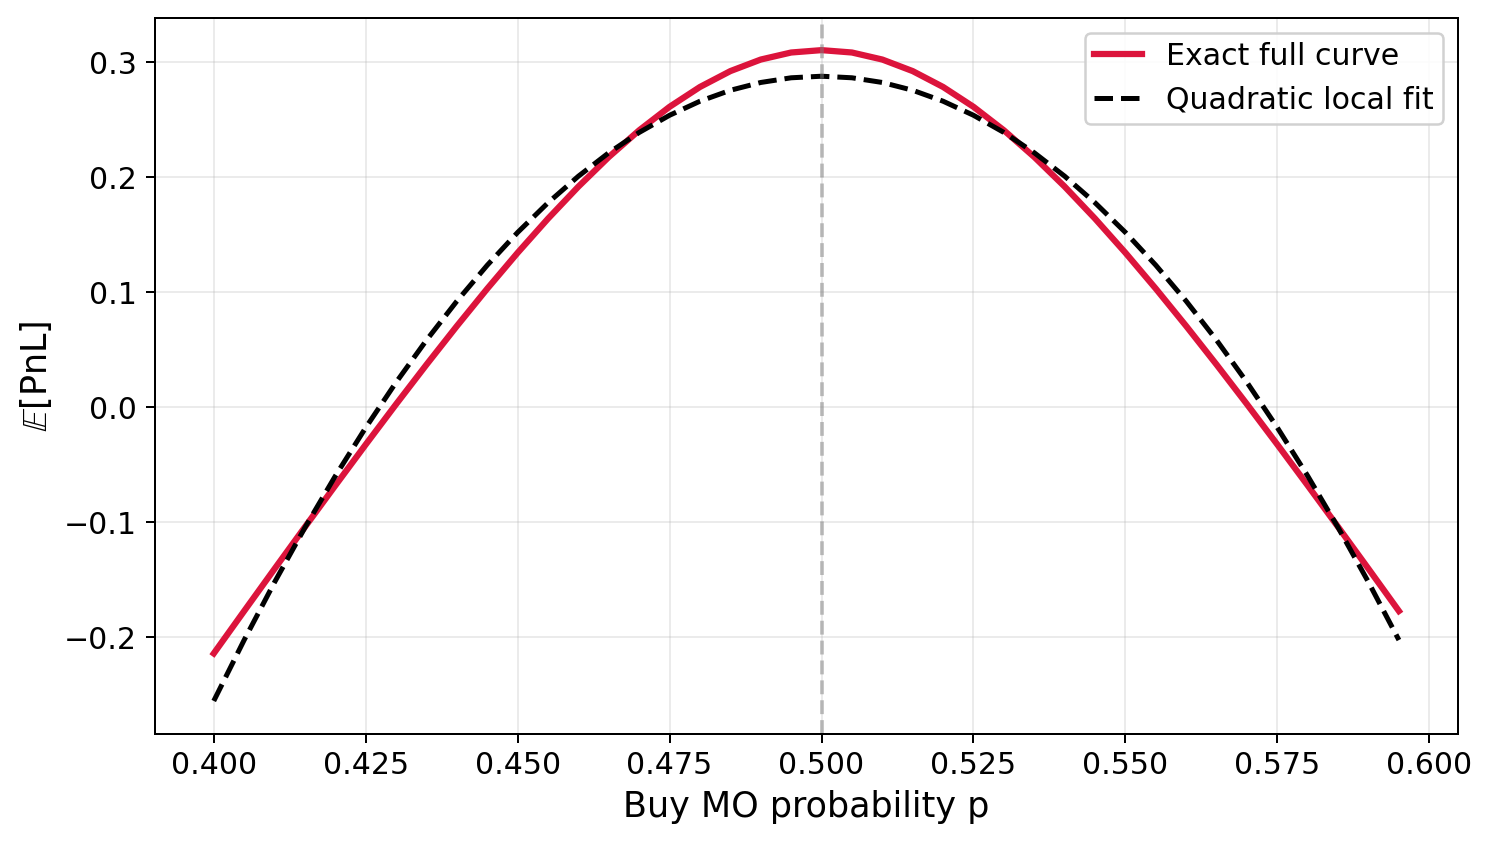
\includegraphics[width=0.60\linewidth]{as_miss_local_quadratic_fit.png}
  \caption{Exact drift-corrected misspecification curve and local
  quadratic approximation around $p=1/2$.  The expansion captures the
  central region, while higher-order boundary and drift effects become
  visible farther into the more asymmetric specifications.}
  \label{fig:app_miss_local_quadratic}
\end{figure}

\end{document}
